
\partabstract{这是大学物理学（第二版）的习题解答。}

\part{大学物理学（第二版）习题解答}

\chapter{第一章 绪论}

1. (a) $1\text{ps} = 10^{-12}\text{s}, 1\text{fs} = 10^{-15}\text{s}$;
(b) $1\text{nm} = 10^{-9}\text{m}$;
(c) $1\text{MeV} = 10^6\text{eV}, 1\text{GeV} = 10^9\text{eV}$

3. $6.022 \times 10^{24}\text{kg}; 0.702\%$

5. $3.16 \times 10^5\text{m}$

7. $t_p = \frac{\hbar}{c^2}\sqrt{\frac{G}{\hbar c}}; \quad m_p = \sqrt{\frac{\hbar c}{G}}$

9. $r = \frac{1}{4\pi\varepsilon_0}\frac{e^2}{m_e c^2} = 2.82 \times 10^{-15}\text{m}$

11. $p \propto \frac{mv^2}{V}f(N)$

17. $b_i \cdot a_j = 2\pi\delta_{ij} \quad \delta_{ij} = \begin{cases} 0 & i \neq j \\ 1 & i = j \end{cases}$

19. $\omega = -\frac{q}{m}B$

21. $1.62 \times 10^4\text{km}$

\begin{exercise}\label{ex:1.1}
为了方便起见，第十四届国际计量大会推荐了如表 1.6 所示的国际单位的词头(SI prefixes)．我们熟悉的 km(kilometer)、cm(centimeter)都是加词头的单位．

(a) 皮秒光学、飞秒光学各涉及什么时间量级?

(b) 纳米(nanometer)材料涉及什么量级的尺度?

(c) eV(电子伏)是能量单位, MeV 和 GeV 分别是多少 eV?
\end{exercise}
\begin{table}[htbp]
\centering
\caption{SI 词头}
\begin{tabular}{llc|llc}
\hline
因数 & 词头名称 & 符号 & 因数 & 词头名称 & 符号 \\
\hline
$10^1$ & 十 & deca (da) & $10^{-1}$ & 分 & deci (d) \\
$10^2$ & 百 & hecto (h) & $10^{-2}$ & 厘 & centi (c) \\
$10^3$ & 千 & kilo (k) & $10^{-3}$ & 毫 & milli (m) \\
$10^6$ & 兆 & mega (M) & $10^{-6}$ & 微 & micro ($\mu$) \\
$10^9$ & 吉 & giga (G) & $10^{-9}$ & 纳 & nano (n) \\
$10^{12}$ & 太 & tera (T) & $10^{-12}$ & 皮 & pico (p) \\
$10^{15}$ & 拍 & peta (P) & $10^{-15}$ & 飞 & femto (f) \\
$10^{18}$ & 艾 & exa (E) & $10^{-18}$ & 阿 & atto (a) \\
\hline
\end{tabular}
\end{table}

\begin{solution}
(a) 根据表格可知，“皮”对应的因数为 $10^{-12}$，“飞”对应的因数为 $10^{-15}$。因此，皮秒光学涉及的时间量级为 $10^{-12}\text{ s}$，飞秒光学涉及的时间量级为 $10^{-15}\text{ s}$。

(b) “纳”对应的因数为 $10^{-9}$，因此纳米材料涉及的尺度量级为 $10^{-9}\text{ m}$。

(c) “兆(M)”对应的因数为 $10^6$，“吉(G)”对应的因数为 $10^9$。因此，$\text{MeV} = 10^6\text{ eV}$，$\text{GeV} = 10^9\text{ eV}$。
\end{solution}

\begin{exercise}\label{ex:1.2}
哈勃半径给出了可观察宇宙半径的量级，它相当于多少 l.y.(光年)?
\end{exercise}
\begin{solution}
哈勃半径 $R_H$ 的量级约为 $10^{26}\text{ m}$。

已知 1 光年 (l.y.) 是光在真空中一年走过的距离，即：
$$ 1\text{ l.y.} = c \times 1\text{ a} \approx 3.0 \times 10^8\text{ m/s} \times 3.156 \times 10^7\text{ s} \approx 9.46 \times 10^{15}\text{ m} $$

因此，哈勃半径相当于：
$$ R_H \approx \frac{10^{26}\text{ m}}{9.46 \times 10^{15}\text{ m/l.y.}} \approx 1.06 \times 10^{10}\text{ l.y.} $$
即大约相当于 100 亿光年。
\end{solution}

\begin{exercise}\label{ex:1.3}
地球的质量是 $5.98 \times 10^{24}\text{ kg}$．利用阿伏伽德罗常量，我们可以说它近似为 $10\text{ mol}$ 个千克．按这一说法，地球的质量是多少? 其精度如何?
\end{exercise}
\begin{solution}
阿伏伽德罗常量 $N_A \approx 6.022 \times 10^{23}\text{ mol}^{-1}$。

按题意，“$10\text{ mol}$ 个千克”对应的质量近似值为：
$$ M' = 10\text{ mol} \times N_A \times 1\text{ kg} \approx 10 \times 6.022 \times 10^{23}\text{ kg} = 6.022 \times 10^{24}\text{ kg} $$

其百分误差（精度）为：
$$ \eta = \frac{|M' - M|}{M} \times 100\% = \frac{|6.022 - 5.98|}{5.98} \times 100\% \approx 0.7\% $$
即这种近似说法的误差不到 $1\%$，精度较高。
\end{solution}

\begin{exercise}\label{ex:1.4}
$1\text{ a}$(一年)近似等于 $\pi \times 10^7\text{ s}$，这一近似的百分误差是多少?
\end{exercise}
\begin{solution}
一年（按回归年计算）的精确时间大约为：
$$ 1\text{ a} = 365.2422\text{ 天} \times 24\text{ h/天} \times 3600\text{ s/h} \approx 31556926\text{ s} $$

近似值 $T' = \pi \times 10^7\text{ s} \approx 3.1415926 \times 10^7\text{ s} = 31415926\text{ s}$。

百分误差为：
$$ \eta = \frac{|T' - T|}{T} \times 100\% = \frac{31556926 - 31415926}{31556926} \times 100\% \approx 0.45\% $$
\end{solution}

\begin{exercise}\label{ex:1.5}
质子的半径约 $10^{-15}\text{ m}$，哈勃半径约为 $10^{26}\text{ m}$，在对数标度上，居间的距离是多少? 试举出这样大小的一个有物理意义的量．
\end{exercise}
\begin{solution}
在对数标度上求居间值，即求这两个量级指数的算术平均值。
$$ \log_{10} R_{\text{mid}} = \frac{-15 + 26}{2} = 5.5 $$
因此，居间的距离 $R_{\text{mid}} = 10^{5.5}\text{ m} \approx 3.16 \times 10^5\text{ m} = 316\text{ km}$。

具有这样大小物理意义的量可以是：某些近地人造卫星的轨道高度，或者是地球上两个相邻城市之间的距离。
\end{solution}

\begin{exercise}\label{ex:1.6}
无量纲量可以有单位，试举两个这方面的例子．
\end{exercise}
\begin{solution}
1. 平面角：其定义为弧长与半径之比 ($l/r$)，量纲为 $1$，但其单位为弧度 (rad)。
2. 立体角：其定义为球面面积与半径平方之比 ($S/r^2$)，量纲为 $1$，但其单位为球面度 (sr)。
\end{solution}

\begin{exercise}\label{ex:1.7}
用三个普适常量分别构造具有：(a) 时间量纲的量；(b) 质量量纲的量．
\end{exercise}
\begin{solution}
我们选取真空中的光速 $c$、万有引力常量 $G$ 和约化普朗克常量 $\hbar$ 作为三个普适常量。它们的量纲分别为：$[c] = \text{L}\text{T}^{-1}$，$[G] = \text{M}^{-1}\text{L}^3\text{T}^{-2}$，$[\hbar] = \text{M}\text{L}^2\text{T}^{-1}$。

(a) 构造具有时间量纲的量（普朗克时间）：
$$ t_p = \sqrt{\frac{\hbar G}{c^5}} $$

(b) 构造具有质量量纲的量（普朗克质量）：
$$ m_p = \sqrt{\frac{\hbar c}{G}} $$
\end{solution}

\begin{exercise}\label{ex:1.8}
利用一球状质量分布的参数 $(m, R)$ 和常数 $G$ 构造一个具有速度量纲的量．
\end{exercise}
\begin{solution}
已知常量的量纲：$[m] = \text{M}$，$[R] = \text{L}$，$[G] = \text{M}^{-1}\text{L}^3\text{T}^{-2}$。速度的量纲为 $[v] = \text{L}\text{T}^{-1}$。

设 $v \propto G^\alpha m^\beta R^\gamma$，则其量纲等式为：
$$ \text{L}\text{T}^{-1} = (\text{M}^{-1}\text{L}^3\text{T}^{-2})^\alpha \text{M}^\beta \text{L}^\gamma = \text{M}^{-\alpha+\beta}\text{L}^{3\alpha+\gamma}\text{T}^{-2\alpha} $$
比较等式两边各基本量纲的指数，可得：
$$ \begin{cases} -\alpha + \beta = 0 \\ 3\alpha + \gamma = 1 \\ -2\alpha = -1 \end{cases} $$
解得 $\alpha = 1/2$，$\beta = 1/2$，$\gamma = -1/2$。

因此，构造出的具有速度量纲的量为 $\sqrt{\frac{Gm}{R}}$。（物理上这对应于环绕速度或逃逸速度的量级）。
\end{solution}

\begin{exercise}\label{ex:1.9}
$m_e c^2$ 是和电子相联系的特征能量，你能否据此定义一个电子“半径”?
\end{exercise}
\begin{solution}
可以。我们可以将电子的特征静止能量 $m_e c^2$ 与电子的静电势能相联系。

假设电子是一个半径为 $r$ 的带电球体，其静电势能的量级为 $\frac{e^2}{4\pi\varepsilon_0 r}$（其中 $e$ 为基本电荷）。令这两者相等：
$$ m_e c^2 = \frac{e^2}{4\pi\varepsilon_0 r} $$
由此可定义出电子的经典半径 $r_e$：
$$ r_e = \frac{e^2}{4\pi\varepsilon_0 m_e c^2} $$
\end{solution}

\begin{exercise}\label{ex:1.10}
一质量为 $m$ 的物体悬挂在劲度系数为 $k$ 的弹簧下面，物体受力正比于其位移，比例系数即为 $k$．利用量纲分析，求出物体-弹簧系统的振动周期 $T$ 对 $k$、$m$ 等量的依赖关系(忽略摩擦)．
\end{exercise}
\begin{solution}
各物理量的量纲为：$[T] = \text{T}$，$[m] = \text{M}$。
由胡克定律 $F = kx$ 可知，劲度系数 $k$ 的量纲为：$[k] = \frac{[F]}{[x]} = \frac{\text{M}\text{L}\text{T}^{-2}}{\text{L}} = \text{M}\text{T}^{-2}$。

假设振动周期 $T = C m^\alpha k^\beta$（其中 $C$ 为无量纲常数），则量纲关系为：
$$ \text{T} = \text{M}^\alpha (\text{M}\text{T}^{-2})^\beta = \text{M}^{\alpha+\beta} \text{T}^{-2\beta} $$
比较两边指数得：
$$ \begin{cases} \alpha + \beta = 0 \\ -2\beta = 1 \end{cases} $$
解得 $\beta = -1/2$，$\alpha = 1/2$。

因此，振动周期 $T$ 对 $k$、$m$ 的依赖关系为：
$$ T \propto \sqrt{\frac{m}{k}} $$
\end{solution}

\begin{exercise}\label{ex:1.11}
一个容积为 $V$ 的盒子内盛有 $N$ 个质量为 $m$ 的粒子，粒子无规地在各个方向上以速率 $v$ 运动．利用量纲分析法，求出这种气体的压强对 $N$、$V$、$m$ 和 $v$ 的依赖关系．
\end{exercise}
\begin{solution}
各物理量的量纲如下：压强 $[p] = \text{M}\text{L}^{-1}\text{T}^{-2}$，容积 $[V] = \text{L}^3$，质量 $[m] = \text{M}$，速率 $[v] = \text{L}\text{T}^{-1}$。粒子数 $N$ 是无量纲量。

假设单粒子对压强的贡献式为 $p' = C V^\alpha m^\beta v^\gamma$，则：
$$ \text{M}\text{L}^{-1}\text{T}^{-2} = (\text{L}^3)^\alpha \text{M}^\beta (\text{L}\text{T}^{-1})^\gamma = \text{M}^\beta \text{L}^{3\alpha+\gamma} \text{T}^{-\gamma} $$
比较指数可得：
$$ \begin{cases} \beta = 1 \\ 3\alpha + \gamma = -1 \\ -\gamma = -2 \end{cases} $$
解得 $\beta = 1$，$\gamma = 2$，$\alpha = -1$。因此 $p' \propto \frac{mv^2}{V}$。

考虑到系统内共有 $N$ 个粒子，总压强应与粒子数成正比，因此压强 $p$ 的依赖关系为：
$$ p \propto \frac{N m v^2}{V} $$
\end{solution}

\begin{exercise}\label{ex:1.12}
低温下固体的热容与温度有关: $C_V = \alpha T^3 + \gamma T$, 其中 $\alpha$、$\gamma$ 为常量．在极低温下，它和温度的什么函数有相同的数量级?
\end{exercise}
\begin{solution}
在极低温（即 $T \to 0$）的条件下，高阶项 $T^3$ 的下降速度远快于线性项 $T$。

因此，当 $T$ 极小时，$\alpha T^3 \ll \gamma T$，热容公式中的线性项 $\gamma T$ 将占据主导地位。故在极低温下，$C_V$ 和温度的一次函数 $T$ 有相同的数量级。
\end{solution}

\begin{exercise}\label{ex:1.13}
展开 $(a^2 - 2ar\cos\theta + r^2)^{-1/2}$ 到二级小量 $(r/a)^2$ $(r \ll a)$．
\end{exercise}
\begin{solution}
首先将原式提出公因子 $a$：
$$ (a^2 - 2ar\cos\theta + r^2)^{-1/2} = \frac{1}{a} \left[ 1 - 2\left(\frac{r}{a}\right)\cos\theta + \left(\frac{r}{a}\right)^2 \right]^{-1/2} $$

令 $x = -2\left(\frac{r}{a}\right)\cos\theta + \left(\frac{r}{a}\right)^2$，由于 $r \ll a$，此 $x$ 为小量。利用泰勒展开公式 $(1+x)^{-1/2} \approx 1 - \frac{1}{2}x + \frac{3}{8}x^2$ 进行展开：
$$ \begin{aligned}
(1+x)^{-1/2} &\approx 1 - \frac{1}{2}\left[ -2\left(\frac{r}{a}\right)\cos\theta + \left(\frac{r}{a}\right)^2 \right] + \frac{3}{8}\left[ -2\left(\frac{r}{a}\right)\cos\theta + \left(\frac{r}{a}\right)^2 \right]^2 \\
&\approx 1 + \left(\frac{r}{a}\right)\cos\theta - \frac{1}{2}\left(\frac{r}{a}\right)^2 + \frac{3}{8}\left[ 4\left(\frac{r}{a}\right)^2\cos^2\theta \right] \quad \text{(舍去高于二次的项)} \\
&= 1 + \left(\frac{r}{a}\right)\cos\theta + \left(\frac{r}{a}\right)^2 \left( \frac{3\cos^2\theta - 1}{2} \right)
\end{aligned} $$

所以，展开式为：
$$ \frac{1}{a} \left[ 1 + \left(\frac{r}{a}\right)\cos\theta + \frac{3\cos^2\theta - 1}{2} \left(\frac{r}{a}\right)^2 \right] $$
\end{solution}

\begin{exercise}\label{ex:1.14}
$\boldsymbol{A}$、$\boldsymbol{B}$、$\boldsymbol{C}$ 都是极矢量，三重积 $\boldsymbol{A} \times (\boldsymbol{B} \times \boldsymbol{C})$ 是极矢量还是轴矢量?
\end{exercise}
\begin{solution}
根据矢量的性质，极矢量与极矢量的叉乘结果是轴矢量（伪矢量），而极矢量与轴矢量的叉乘结果是极矢量。

题中 $\boldsymbol{B}$ 和 $\boldsymbol{C}$ 均为极矢量，故它们的叉积 $(\boldsymbol{B} \times \boldsymbol{C})$ 是轴矢量。
$\boldsymbol{A}$ 是极矢量，故极矢量 $\boldsymbol{A}$ 与轴矢量 $(\boldsymbol{B} \times \boldsymbol{C})$ 的叉积必然是极矢量。
\end{solution}

\begin{exercise}\label{ex:1.15}
作图说明: 混合积 $\boldsymbol{A} \cdot (\boldsymbol{B} \times \boldsymbol{C})$ 表示平行六面体的体积．
\end{exercise}
\begin{proof}
设由不共面的三个矢量 $\boldsymbol{A}, \boldsymbol{B}, \boldsymbol{C}$ 构成一个平行六面体。

1. 考虑底面由矢量 $\boldsymbol{B}$ 和 $\boldsymbol{C}$ 构成，由叉乘的几何意义可知，$\boldsymbol{B} \times \boldsymbol{C}$ 的模长 $|\boldsymbol{B} \times \boldsymbol{C}|$ 在数值上等于该底面平行四边形的面积 $S$。且矢量 $\boldsymbol{B} \times \boldsymbol{C}$ 的方向垂直于底面，即为该平行六面体的高的方向（法线方向 $\boldsymbol{n}$）。
2. 平行六面体的高 $h$ 等于矢量 $\boldsymbol{A}$ 在法线 $\boldsymbol{n}$ 方向上的投影，即 $h = |\boldsymbol{A}| \cos\theta$，其中 $\theta$ 是 $\boldsymbol{A}$ 与 $\boldsymbol{B} \times \boldsymbol{C}$ 之间的夹角。
3. 根据点乘的定义，混合积可写为：
$$ \boldsymbol{A} \cdot (\boldsymbol{B} \times \boldsymbol{C}) = |\boldsymbol{A}| |\boldsymbol{B} \times \boldsymbol{C}| \cos\theta = (|\boldsymbol{B} \times \boldsymbol{C}|) \cdot (|\boldsymbol{A}| \cos\theta) = S \cdot h $$
这正是底面积乘以高，即平行六面体的体积。
\end{proof}

\begin{exercise}\label{ex:1.16}
当矢量 $\boldsymbol{A}$、$\boldsymbol{B}$、$\boldsymbol{C}$ 作镜像变换时，混合积 $\boldsymbol{A} \cdot (\boldsymbol{B} \times \boldsymbol{C})$ 如何变换? 设该混合积为非零的量．
\end{exercise}
\begin{solution}
设 $\boldsymbol{A}, \boldsymbol{B}, \boldsymbol{C}$ 为极矢量，在坐标系的镜像变换（即空间反演）下，极矢量会反向，即 $\boldsymbol{A} \to -\boldsymbol{A}$，$\boldsymbol{B} \to -\boldsymbol{B}$，$\boldsymbol{C} \to -\boldsymbol{C}$。

对混合积进行代入变换：
$$ (-\boldsymbol{A}) \cdot ((-\boldsymbol{B}) \times (-\boldsymbol{C})) = (-\boldsymbol{A}) \cdot (\boldsymbol{B} \times \boldsymbol{C}) = - \left[ \boldsymbol{A} \cdot (\boldsymbol{B} \times \boldsymbol{C}) \right] $$
由此可见，混合积在镜像变换下改变符号。这表明该混合积是一个伪标量（赝标量）。
\end{solution}

\begin{exercise}\label{ex:1.17}
已知矢量
$$ \boldsymbol{b}_1 = 2\pi \frac{\boldsymbol{a}_2 \times \boldsymbol{a}_3}{\boldsymbol{a}_1 \cdot (\boldsymbol{a}_2 \times \boldsymbol{a}_3)}, \quad \boldsymbol{b}_2 = 2\pi \frac{\boldsymbol{a}_3 \times \boldsymbol{a}_1}{\boldsymbol{a}_1 \cdot (\boldsymbol{a}_2 \times \boldsymbol{a}_3)}, \quad \boldsymbol{b}_3 = 2\pi \frac{\boldsymbol{a}_1 \times \boldsymbol{a}_2}{\boldsymbol{a}_1 \cdot (\boldsymbol{a}_2 \times \boldsymbol{a}_3)} $$
试归纳出标量积 $\boldsymbol{b}_i \cdot \boldsymbol{a}_j$ 值满足的规律．
\end{exercise}
\begin{solution}
分别计算 $\boldsymbol{b}_i \cdot \boldsymbol{a}_j$ 的值：

当 $i = j$ 时，例如 $i=1, j=1$：
$$ \boldsymbol{b}_1 \cdot \boldsymbol{a}_1 = 2\pi \frac{(\boldsymbol{a}_2 \times \boldsymbol{a}_3) \cdot \boldsymbol{a}_1}{\boldsymbol{a}_1 \cdot (\boldsymbol{a}_2 \times \boldsymbol{a}_3)} = 2\pi \frac{\boldsymbol{a}_1 \cdot (\boldsymbol{a}_2 \times \boldsymbol{a}_3)}{\boldsymbol{a}_1 \cdot (\boldsymbol{a}_2 \times \boldsymbol{a}_3)} = 2\pi $$
同理可证 $\boldsymbol{b}_2 \cdot \boldsymbol{a}_2 = 2\pi$，$\boldsymbol{b}_3 \cdot \boldsymbol{a}_3 = 2\pi$。

当 $i \neq j$ 时，例如 $i=1, j=2$：
$$ \boldsymbol{b}_1 \cdot \boldsymbol{a}_2 = 2\pi \frac{(\boldsymbol{a}_2 \times \boldsymbol{a}_3) \cdot \boldsymbol{a}_2}{\boldsymbol{a}_1 \cdot (\boldsymbol{a}_2 \times \boldsymbol{a}_3)} $$
因为 $(\boldsymbol{a}_2 \times \boldsymbol{a}_3)$ 生成的矢量垂直于 $\boldsymbol{a}_2$ 和 $\boldsymbol{a}_3$，所以 $(\boldsymbol{a}_2 \times \boldsymbol{a}_3) \cdot \boldsymbol{a}_2 = 0$，结果为 $0$。同理，所有 $i \neq j$ 的项点积皆为 $0$。

归纳规律可表示为克罗内克 $\delta$ 函数形式：
$$ \boldsymbol{b}_i \cdot \boldsymbol{a}_j = 2\pi \delta_{ij} \quad \text{其中} \quad \delta_{ij} = \begin{cases} 1, & i = j \\ 0, & i \neq j \end{cases} $$
\end{solution}

\begin{exercise}\label{ex:1.18}
求例 1.3 中的 $\boldsymbol{A}$、$\boldsymbol{d}$．
\end{exercise}
\begin{solution}
由于题干未提供教材“例 1.3”的具体数值与上下文，此处省略具体数值计算。一般情况下，求矢量的模长和方向可以通过相应的矢量代数公式代入数据进行求解，如需精确解答请补充“例 1.3”的内容。
\end{solution}

\begin{exercise}\label{ex:1.19}
电荷在已知磁场 $\boldsymbol{B}$ 中的运动遵循
$$ m\boldsymbol{a} = q\boldsymbol{v} \times \boldsymbol{B} $$
如果加速度 $\boldsymbol{a}$ 可以表示为 $\boldsymbol{\omega} \times \boldsymbol{v}$，其中矢量 $\boldsymbol{\omega}$ 怎样用已知矢量 $\boldsymbol{B}$ 来表达?
\end{exercise}
\begin{solution}
已知 $m\boldsymbol{a} = q\boldsymbol{v} \times \boldsymbol{B}$，将 $\boldsymbol{a} = \boldsymbol{\omega} \times \boldsymbol{v}$ 代入方程：
$$ m(\boldsymbol{\omega} \times \boldsymbol{v}) = q\boldsymbol{v} \times \boldsymbol{B} $$
利用叉乘反交换律 $\boldsymbol{v} \times \boldsymbol{B} = -\boldsymbol{B} \times \boldsymbol{v}$，等式右侧可改写为：
$$ m(\boldsymbol{\omega} \times \boldsymbol{v}) = -q(\boldsymbol{B} \times \boldsymbol{v}) $$
由于此等式对任意速度 $\boldsymbol{v}$ 均成立，故可去掉两边的叉乘项（对比系数），得到：
$$ m\boldsymbol{\omega} = -q\boldsymbol{B} $$
解得矢量 $\boldsymbol{\omega}$：
$$ \boldsymbol{\omega} = -\frac{q}{m}\boldsymbol{B} $$
这正是回旋加速频率（矢量形式）的表达式。
\end{solution}

\begin{exercise}\label{ex:1.20}
证明：2 个线性相关的矢量一定共线，3 个线性相关的矢量一定共面．
\end{exercise}
\begin{proof}
(1) 设 2 个矢量 $\boldsymbol{A}$ 和 $\boldsymbol{B}$ 线性相关，则存在不全为零的常数 $c_1, c_2$，使得：
$$ c_1 \boldsymbol{A} + c_2 \boldsymbol{B} = \boldsymbol{0} $$
不妨设 $c_1 \neq 0$，则有 $\boldsymbol{A} = -\frac{c_2}{c_1} \boldsymbol{B}$。这说明矢量 $\boldsymbol{A}$ 是矢量 $\boldsymbol{B}$ 的标量倍，故它们方向相同或相反，即一定共线。

(2) 设 3 个矢量 $\boldsymbol{A}, \boldsymbol{B}, \boldsymbol{C}$ 线性相关，则存在不全为零的常数 $c_1, c_2, c_3$，使得：
$$ c_1 \boldsymbol{A} + c_2 \boldsymbol{B} + c_3 \boldsymbol{C} = \boldsymbol{0} $$
不妨设 $c_3 \neq 0$，则有 $\boldsymbol{C} = -\frac{c_1}{c_3} \boldsymbol{A} - \frac{c_2}{c_3} \boldsymbol{B}$。这说明矢量 $\boldsymbol{C}$ 可以由矢量 $\boldsymbol{A}$ 和 $\boldsymbol{B}$ 线性表出。根据矢量的加法规则，能够由另外两个不共线矢量表出的矢量，必然位于那两个矢量所决定的平面内。因此，它们一定共面。
\end{proof}

\begin{exercise}\label{ex:1.21}
一人从悉尼去波士顿旅行，两个城市的纬度和经度分别为(34S, 151E)和(42N, 71W)．出发和到达时的位置矢量是什么(用球坐标表示)? 位移矢量又是什么? 取地球平均半径为 $6.370 \times 10^3\text{ km}$，问两城市间的直线距离是多少?
\end{exercise}
\begin{solution}
建立球坐标系 $(r, \theta, \phi)$：极轴指向北极（$\theta=0^\circ$），赤道平面为 $\theta=90^\circ$；本初子午线对应 $\phi=0^\circ$，向东为正，向西为负。

(1) 位置矢量：
悉尼 (34S, 151E)：极角 $\theta_1 = 90^\circ + 34^\circ = 124^\circ$，方位角 $\phi_1 = 151^\circ$。
出发位置矢量：$\boldsymbol{r}_1 = (R, 124^\circ, 151^\circ)$。
波士顿 (42N, 71W)：极角 $\theta_2 = 90^\circ - 42^\circ = 48^\circ$，方位角 $\phi_2 = -71^\circ = 289^\circ$。
到达位置矢量：$\boldsymbol{r}_2 = (R, 48^\circ, -71^\circ)$。

(2) 位移矢量：
位移矢量为 $\Delta\boldsymbol{r} = \boldsymbol{r}_2 - \boldsymbol{r}_1$。

(3) 直线距离：
直线距离 $d = |\Delta\boldsymbol{r}| = |\boldsymbol{r}_2 - \boldsymbol{r}_1| = \sqrt{R^2 + R^2 - 2R^2\cos\gamma} = R\sqrt{2 - 2\cos\gamma}$，
其中 $\gamma$ 为两位置矢量夹角，利用球面三角公式或直角坐标点乘计算：
$$ \begin{aligned}
\cos\gamma &= \frac{\boldsymbol{r}_1 \cdot \boldsymbol{r}_2}{R^2} = \sin\theta_1\sin\theta_2\cos(\phi_1-\phi_2) + \cos\theta_1\cos\theta_2 \\
&= \sin(124^\circ)\sin(48^\circ)\cos(151^\circ - (-71^\circ)) + \cos(124^\circ)\cos(48^\circ) \\
&= (0.8290)(0.7431)\cos(222^\circ) + (-0.5592)(0.6691) \\
&\approx 0.6160 \times (-0.7431) - 0.3742 \\
&\approx -0.4578 - 0.3742 = -0.8320
\end{aligned} $$
代入距离公式：
$$ d = R\sqrt{2 - 2(-0.8320)} = R\sqrt{3.664} \approx 1.914R $$
由于 $R = 6.370 \times 10^3\text{ km}$，
$$ d \approx 1.914 \times 6370\text{ km} \approx 12192\text{ km} $$
即两城市间的直线距离约为 $1.22 \times 10^4\text{ km}$。
\end{solution}

\begin{exercise}\label{ex:1.22}
在直角坐标系中有矢量
$$ \boldsymbol{A} = (2, 1, 1), \quad \boldsymbol{B} = (5, 2, 0), \quad \boldsymbol{C} = (1, 1, 1) $$
求：(a) $\boldsymbol{A} \cdot \boldsymbol{B}$, (b) $\boldsymbol{A} \times \boldsymbol{B}$, (c) $\boldsymbol{A} \cdot (\boldsymbol{B} \times \boldsymbol{C})$,
(d) $\boldsymbol{A} \times (\boldsymbol{B} \times \boldsymbol{C})$, (e) $\boldsymbol{A} \cdot (\boldsymbol{A} + \boldsymbol{B} \times \boldsymbol{C})$, (f) $\boldsymbol{A} \cdot (\boldsymbol{B} \times \boldsymbol{C} - \boldsymbol{A} \times \boldsymbol{B})$
\end{exercise}
\begin{solution}
(a) $\boldsymbol{A} \cdot \boldsymbol{B} = 2 \times 5 + 1 \times 2 + 1 \times 0 = 10 + 2 + 0 = 12$。

(b) $\boldsymbol{A} \times \boldsymbol{B} = \begin{vmatrix} \boldsymbol{i} & \boldsymbol{j} & \boldsymbol{k} \\ 2 & 1 & 1 \\ 5 & 2 & 0 \end{vmatrix} = (1 \times 0 - 1 \times 2)\boldsymbol{i} - (2 \times 0 - 1 \times 5)\boldsymbol{j} + (2 \times 2 - 1 \times 5)\boldsymbol{k} = (-2, 5, -1)$。

(c) 先计算 $\boldsymbol{B} \times \boldsymbol{C} = \begin{vmatrix} \boldsymbol{i} & \boldsymbol{j} & \boldsymbol{k} \\ 5 & 2 & 0 \\ 1 & 1 & 1 \end{vmatrix} = (2-0)\boldsymbol{i} - (5-0)\boldsymbol{j} + (5-2)\boldsymbol{k} = (2, -5, 3)$。
则 $\boldsymbol{A} \cdot (\boldsymbol{B} \times \boldsymbol{C}) = 2 \times 2 + 1 \times (-5) + 1 \times 3 = 4 - 5 + 3 = 2$。

(d) $\boldsymbol{A} \times (\boldsymbol{B} \times \boldsymbol{C}) = \begin{vmatrix} \boldsymbol{i} & \boldsymbol{j} & \boldsymbol{k} \\ 2 & 1 & 1 \\ 2 & -5 & 3 \end{vmatrix} = (3 - (-5))\boldsymbol{i} - (6 - 2)\boldsymbol{j} + (-10 - 2)\boldsymbol{k} = (8, -4, -12)$。

(e) $\boldsymbol{A} \cdot (\boldsymbol{A} + \boldsymbol{B} \times \boldsymbol{C}) = \boldsymbol{A} \cdot \boldsymbol{A} + \boldsymbol{A} \cdot (\boldsymbol{B} \times \boldsymbol{C})$。
已知 $\boldsymbol{A} \cdot \boldsymbol{A} = 2^2 + 1^2 + 1^2 = 6$，且由 (c) 知 $\boldsymbol{A} \cdot (\boldsymbol{B} \times \boldsymbol{C}) = 2$，
因此 $\boldsymbol{A} \cdot (\boldsymbol{A} + \boldsymbol{B} \times \boldsymbol{C}) = 6 + 2 = 8$。

(f) $\boldsymbol{A} \cdot (\boldsymbol{B} \times \boldsymbol{C} - \boldsymbol{A} \times \boldsymbol{B}) = \boldsymbol{A} \cdot (\boldsymbol{B} \times \boldsymbol{C}) - \boldsymbol{A} \cdot (\boldsymbol{A} \times \boldsymbol{B})$。
由 (c) 知第一项为 $2$。由于 $\boldsymbol{A} \times \boldsymbol{B}$ 垂直于 $\boldsymbol{A}$，故第二项混合积为 $0$。
因此 $\boldsymbol{A} \cdot (\boldsymbol{B} \times \boldsymbol{C} - \boldsymbol{A} \times \boldsymbol{B}) = 2 - 0 = 2$。
\end{solution}

\chapter{第二章 运动学}

1. $3.91 \times 10^{-2}\text{m}$

3. $22.1\text{m}$

5. $d = v\left(\frac{2\ell \sin\theta}{g}\right)^{1/2} - \ell \cos\theta$

7. $8.98 \times 10^{22}\text{m/s}^2$

9. $387$

13. [图片：等值线图形]

15. $115.37^\circ; 0.21\text{h}$


\begin{exercise}\label{ex:2.1}
一带电粒子以 $3.00 \times 10^6 \ \mathrm{m/s}$ 的速度射入电场区，受到 $1.15 \times 10^{14} \ \mathrm{m/s^2}$ 的逆向加速度. 带电粒子飞行多远后静止？能静止多久？
\end{exercise}
\begin{solution}

\end{solution}

\begin{exercise}\label{ex:2.2}
一自由落体在最后 $1.0 \ \mathrm{s}$ 内通过了其全程距离的一半. 试求出该落体下落的距离及所用时间.
\end{exercise}
\begin{solution}

\end{solution}

\begin{exercise}\label{ex:2.3}
一钢球从一建筑物的屋顶由静止开始自由下落. 建筑物内一观察者站在高度为 $1.3 \ \mathrm{m}$ 的窗前，发现钢球从窗的最上端落至最下端用了 $0.125 \ \mathrm{s}$. 钢球继续下落，$2.0 \ \mathrm{s}$ 后，与水平地面发生完全弹性碰撞并上升至窗的最下端，试求该建筑物的高度.
\end{exercise}
\begin{solution}

\end{solution}

\begin{exercise}\label{ex:2.4}
设计一个实验，利用落体或上抛运动来测量重力加速度 $g$.
\end{exercise}
\begin{solution}

\end{solution}

\begin{exercise}\label{ex:2.5}
一地面雷达观察者正注视一抛射体，在某一时刻，他得到如下信息：抛射体达到了最高点，并具有大小为 $v$ 的水平速度，此时抛射体与观察者的直线距离为 $\ell$，观察者的视线与水平面的夹角为 $\theta$.
\begin{enumerate}
  \item[(a)] 计算抛射体的落地点与观察者的水平距离 $d$，用 $\ell$、$v$、$\theta$ 表示.
  \item[(b)] 抛射体是否能越过观察者的头顶？
\end{enumerate}
\end{exercise}
\begin{solution}

\end{solution}

\begin{exercise}\label{ex:2.6}
蟹状星云中的脉冲星转速为 $30 \ \mathrm{r/s}$，半径为 $150 \ \mathrm{km}$. 位于星体赤道附近物体的加速度是多少？
\end{exercise}
\begin{solution}

\end{solution}

\begin{exercise}\label{ex:2.7}
在玻尔的氢原子模型中，电子围绕原子核作匀速圆周运动，在半径为 $5.29 \times 10^{-11} \ \mathrm{m}$ 的轨道上，其速度为 $2.18 \times 10^6 \ \mathrm{m/s}$，求氢原子中电子的加速度.
\end{exercise}
\begin{solution}

\end{solution}

\begin{exercise}\label{ex:2.8}
由于地球的自转，地球赤道上某一点具有一定的加速度，而地球本身由于绕太阳公转，也具有一定的加速度，试求这两个加速度之比. 假定公转轨道为圆形.
\end{exercise}
\begin{solution}

\end{solution}

\begin{exercise}\label{ex:2.9}
一音叉与频率为 $384 \ \mathrm{Hz}$ 的标准音叉形成每秒三次的拍频. 当这一音叉的一支粘上一小块蜡时，拍频降低. 问这音叉的频率是多少？
\end{exercise}
\begin{solution}

\end{solution}

\begin{exercise}\label{ex:2.10}
试写一程序演示李萨如图形. 可取 $x=\cos(2\pi \cdot 1 \cdot t+0)$，垂直振动频率和初相位作可调参数.
\end{exercise}
\begin{solution}

\end{solution}

\begin{exercise}\label{ex:2.11}
试作正交相差的两振动的矢量和位移叠加图.
\end{exercise}
\begin{solution}

\end{solution}

\begin{exercise}\label{ex:2.12}
讨论受周期性冲击的简谐振子. 冲击导致速率的不连续跳变. 它的相空间的轨迹是什么？如果我们只取相空间中 $t=T, 2T, 3T, \dots$ 的点，图形是怎样的？
\end{exercise}
\begin{solution}

\end{solution}

\begin{exercise}\label{ex:2.13}
在双阱势中，运动的相图是怎样的？
\end{exercise}
\begin{solution}

\end{solution}

\begin{exercise}\label{ex:2.14}
飞行员从 A 地向正东飞行至 B 地，然后返回. 空气相对于地面的速度是 $u$，而飞机相对于空气的速度 $v'$ 为常量. 试对风速：
\begin{enumerate}
  \item[(a)] 为零；
  \item[(b)] 正东；
  \item[(c)] 正北，求来回飞行时间.
\end{enumerate}
在后两种情形，对 $v'$ 有什么要求？
\end{exercise}
\begin{solution}

\end{solution}

\begin{exercise}\label{ex:2.15}
一人欲划船渡过 $500 \ \mathrm{m}$ 宽的河流. 他相对于水的速度为 $3000 \ \mathrm{m/h}$，水流速度为 $2000 \ \mathrm{m/h}$. 设人在岸上的行走速度为 $5000 \ \mathrm{m/h}$，
\begin{enumerate}
  \item[(a)] 为了在最短时间内达到河对岸正对出发点的位置，此人需选择怎样的路线？
  \item[(b)] 该最短时间为多少？
\end{enumerate}
\end{exercise}
\begin{solution}

\end{solution}

\begin{exercise}\label{ex:2.16}
一质量为 $m$ 的病毒微粒存在于某溶液中，盛该溶液的试管置于一离心机上. 离心机以每分钟 $n$ 转的速率旋转. 在某个时刻，该病毒位于距旋转轴 $r$ 处，并相对于试管以恒定速率 $v_0$ 沿径向运动. 试分别在下面两个参考系中，定量地考虑病毒的运动情形并给出所有受力大小：
\begin{enumerate}
  \item[(a)] 随离心机一同旋转的参考系；
  \item[(b)] 固定的实验室参考系.
\end{enumerate}
\end{exercise}
\begin{solution}

\end{solution}

\chapter{第三章 质点动力学}

3. (a) (b) $g\sin\theta$
(c) $(g - a)\sin\theta$
(d) $(g + a)\sin\theta$
(e) $0$
(f) $m(g - a)\cos\theta$

5. (a) $mg/k$
(b) $v = v_T(1 - \text{e}^{-kt/m})$
(c) $g \text{e}^{-kt/m}$
(d) $y = v_T t + v_T \left(\frac{m}{k}\right) (\text{e}^{-kt/m} - 1)$

7. (a) $0$
(b) $\alpha \approx 3.0 \times 10^{-3}\lambda$
(c) $0$

9. $x = 2.20 \times 10^{-5}h^{3/2}\sin\theta$

11. (a) $F(r) = \frac{U}{r} \left( 1 + \frac{r}{r_0} \right)$
(b) $0.14, 7.8 \times 10^{-3}, 6.8 \times 10^{-6}$

13. (a) $v_0 \ge \sqrt{5gR} \equiv v_m$
(b) $\theta = 19^\circ 32'$

\begin{exercise}\label{ex:3.1}
两个质量均为 $m$ 的质点，由长度为 $2\ell$ 的轻绳连接，一恒力 $\boldsymbol{F}$ 持续地垂直作用于细绳的中点($x=0$)处（如图）. 证明每一个质点在与作用力 $\boldsymbol{F}$ 垂直的方向上的加速度的大小为
$$a_x = - \frac{F}{2m} \frac{x}{\sqrt{\ell^2 - x^2}}$$
式中 $x$ 是质点与 $\boldsymbol{F}$ 的垂直距离. 讨论当 $x=\ell$ 时的情形.
\begin{center}
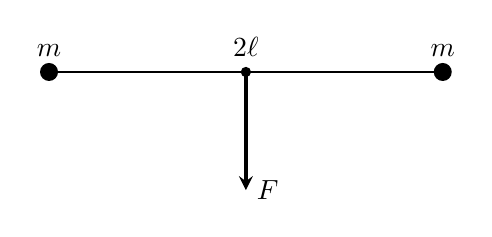
\begin{tikzpicture}[>=stealth, thick]
    \def\L{2.5}
    % String
    \draw (-\L,0) -- (\L,0);
    % Masses
    \filldraw[black] (-\L,0) circle (0.1) node[above=2pt] {$m$};
    \filldraw[black] (\L,0) circle (0.1) node[above=2pt] {$m$};
    % Center point
    \filldraw[black] (0,0) circle (0.05);
    \node[above=2pt] at (0,0) {$2\ell$};
    % Force
    \draw[->, very thick] (0,0) -- (0,-1.5) node[right] {$\boldsymbol{F}$};
\end{tikzpicture}
\end{center}
\end{exercise}
\begin{solution}

\end{solution}

\begin{exercise}\label{ex:3.2}
一质量为 $m'$、角度为 $\theta$ 的楔块置于水平桌面上，另一质量为 $m$ 的立方块放在该楔块的斜面上，见图. 假设所有的接触面都是光滑的，
\begin{enumerate}
  \item[(a)] 为使立方块相对于斜面静止，则该楔块应以多大的水平加速度运动？
  \item[(b)] 此时作用于该系统上的水平作用力 $\boldsymbol{F}$ 是多少？如果没有任何外力作用于该系统，试描述楔块 $m'$ 和立方块 $m$ 的运动.
\end{enumerate}
\begin{center}
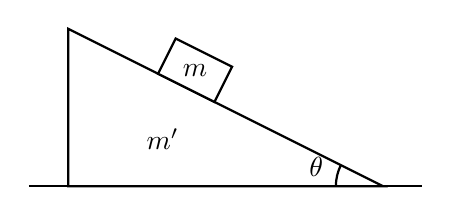
\begin{tikzpicture}[>=stealth, thick]
    \def\W{4}
    \def\H{2}
    % Ground
    \draw (-0.5,0) -- (\W+0.5,0);
    % Wedge
    \draw (0,0) -- (\W,0) -- (0,\H) -- cycle;
    \node at (1.2, 0.6) {$m'$};
    % Angle
    \draw (\W-0.6,0) arc (180:153.43:0.6);
    \node at (\W-0.85, 0.25) {$\theta$};
    
    % Block
    \begin{scope}[shift={(1.5, 1.25)}, rotate=-26.57]
        \draw[fill=white] (-0.4,0) rectangle (0.4,0.5);
        \node at (0, 0.25) {$m$};
    \end{scope}
\end{tikzpicture}
\end{center}
\end{exercise}
\begin{solution}

\end{solution}

\begin{exercise}\label{ex:3.3}
升降机中一斜面与地板成 $\theta$ 角. 质量为 $m$ 的立方块从斜面滑下. 在以下情形，求立方块相对于斜面的加速度：升降机
\begin{enumerate}
  \item[(a)] 匀速上升、
  \item[(b)] 匀速下降、
  \item[(c)] 匀加速上升、
  \item[(d)] 匀减速下降、
  \item[(e)] 缆绳断裂.
  \item[(f)] 求在升降机匀加速上升时斜面对立方块的力.
\end{enumerate}
\end{exercise}
\begin{solution}

\end{solution}

\begin{exercise}\label{ex:3.4}
一质量为 $m$ 的小立方块置于旋转漏斗内壁（见图）. 漏斗以 $f$ 旋转. 设漏斗与水平方向的夹角为 $\theta$，立方块与漏斗表面间的摩擦系数为 $\mu$. 求使小立方块不滑动的最大转速 $f_{\max}$ 和最小转速 $f_{\min}$.
\begin{center}
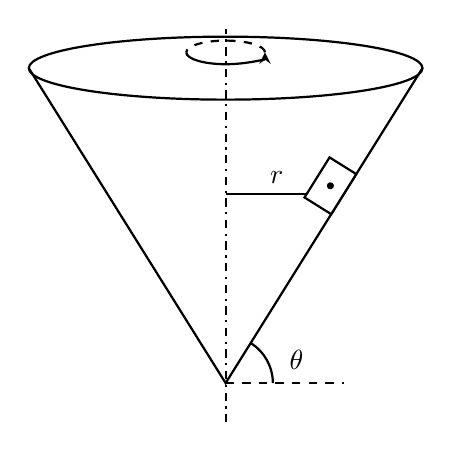
\begin{tikzpicture}[>=stealth, thick]
    \def\W{2.5}
    \def\H{4}
    % Central axis
    \draw[dash dot] (0,-0.5) -- (0,\H+0.5);
    % Rotation arrow
    \draw[->] (-0.5, \H+0.2) arc (180:360:0.5 and 0.15);
    \draw[dashed] (0.5, \H+0.2) arc (0:180:0.5 and 0.15);
    
    % Funnel
    \draw (-\W,\H) -- (0,0) -- (\W,\H);
    \draw (0,\H) ellipse (2.5 and 0.4);
    
    % Horizontal line and angle
    \draw[dashed] (0,0) -- (1.5,0);
    \draw (0.6,0) arc (0:58:0.6);
    \node at (0.9, 0.3) {$\theta$};
    
    % Distance r
    \draw (0, 2.4) -- (1.3, 2.4);
    \node[above] at (0.65, 2.4) {$r$};
    
    % Block
    \begin{scope}[shift={(1.5, 2.4)}, rotate=58]
        \draw[fill=white] (-0.3,0) rectangle (0.3,0.4);
        \filldraw[black] (0,0.2) circle (0.03);
    \end{scope}
\end{tikzpicture}
\end{center}
\end{exercise}
\begin{solution}

\end{solution}

\begin{exercise}\label{ex:3.5}
某物体下落过程中受到空气的阻力 $\boldsymbol{F}_{\mathrm{d}} = -k\boldsymbol{v}$，其中 $v$ 是物体的速度、$k$ 为与速度无关的常量.
\begin{enumerate}
  \item[(a)] 求终极速度；
  \item[(b)] 将速度对时间作图；
  \item[(c)] 将加速度对时间作图；
  \item[(d)] 将下落距离对时间作图.
\end{enumerate}
\end{exercise}
\begin{solution}

\end{solution}

\begin{exercise}\label{ex:3.6}
采用非惯性参考系重解 3.2 题、3.3 题、3.4 题.
\end{exercise}
\begin{solution}

\end{solution}

\begin{exercise}\label{ex:3.7}
由于地球的旋转，铅垂实际上将不再指向地心. 求在
\begin{enumerate}
  \item[(a)] 北极、
  \item[(b)] $30^\circ\mathrm{N}$、
  \item[(c)] 赤道等处的偏离情况.
\end{enumerate}
\end{exercise}
\begin{solution}

\end{solution}

\begin{exercise}\label{ex:3.8}
在北半球，
\begin{enumerate}
  \item[(a)] 求出水平向东运动的物体所受的科里奥利力；
  \item[(b)] 求垂直向上运动的物体所受的科里奥利力.
\end{enumerate}
\end{exercise}
\begin{solution}

\end{solution}

\begin{exercise}\label{ex:3.9}
在北纬 $30^\circ 05'$ 处，一物体从 $10 \ \mathrm{m}$ 高处落下，求由于科里奥利力的作用而引起物体落点的水平偏移量. (空气阻力不计)
\end{exercise}
\begin{solution}

\end{solution}

\begin{exercise}\label{ex:3.10}
水流冲击涡轮机的碟状叶片，冲击前后水的速率均为 $v$，如图所示. 单位时间撞击叶片的水量是常量 $\mu$. 求水施加在叶片上的力.
\begin{center}
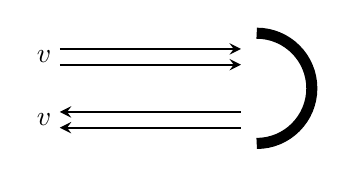
\begin{tikzpicture}[>=stealth, thick]
    % Blade arc
    \draw[line width=4pt] (1,0.7) arc (90:-90:0.7);
    % Incoming water arrows
    \draw[->] (-1.5, 0.5) -- (0.8, 0.5);
    \draw[->] (-1.5, 0.3) -- (0.8, 0.3);
    % Outgoing water arrows
    \draw[->] (0.8, -0.3) -- (-1.5, -0.3);
    \draw[->] (0.8, -0.5) -- (-1.5, -0.5);
    % Label v
    \node at (-1.7, 0.4) {$v$};
    \node at (-1.7, -0.4) {$v$};
\end{tikzpicture}
\end{center}
\end{exercise}
\begin{solution}

\end{solution}

\begin{exercise}\label{ex:3.11}
所谓的汤川(Yukawa)势具有如下形式：
$$U(r) = -\frac{r_0}{r} U_0 \mathrm{e}^{-r/r_0}$$
它相当好地描述了核子间的相互作用. 这里常量 $r_0 = 1.5 \times 10^{-15} \ \mathrm{m}$，$U_0 = 50 \ \mathrm{MeV}$.
\begin{enumerate}
  \item[(a)] 给出相应的作用力的表达式；
  \item[(b)] 说明该种作用力的短程性质，并计算当 $r=2r_0$、$4r_0$ 及 $10r_0$ 时的作用力与 $r=r_0$ 时的作用力之比.
\end{enumerate}
\end{exercise}
\begin{solution}

\end{solution}

\begin{exercise}\label{ex:3.12}
一质点从无摩擦的球面自静止开始下滑，如图所示. 求：
\begin{enumerate}
  \item[(a)] 势能作为角度 $\theta$ 的函数；
  \item[(b)] 动能作为 $\theta$ 的函数；
  \item[(c)] 切向和法向加速度作为 $\theta$ 的函数；
  \item[(d)] 质点飞离球面的角度.
\end{enumerate}
\begin{center}
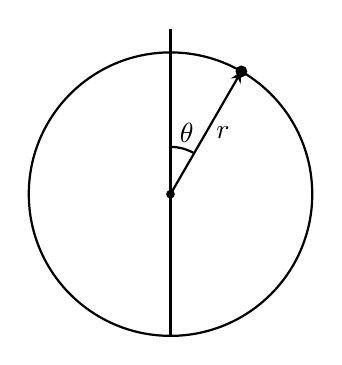
\begin{tikzpicture}[>=stealth, thick]
    \def\R{1.8}
    % Sphere (circle)
    \draw (0,0) circle (\R);
    % Vertical lines
    \draw (0,0) -- (0,\R+0.3);
    \draw (0,0) -- (0,-\R);
    % Radius vector
    \draw[->] (0,0) -- (60:\R) node[midway, right] {$r$};
    % Angle theta
    \draw (0,0.6) arc (90:60:0.6);
    \node at (75:0.8) {$\theta$};
    % Particle and center point
    \filldraw[black] (60:\R) circle (0.06);
    \filldraw[black] (0,0) circle (0.04);
\end{tikzpicture}
\end{center}
\end{exercise}
\begin{solution}

\end{solution}

\begin{exercise}\label{ex:3.13}
如图，一质量为 $m$ 的质点在一光滑的半径为 $r$ 的圆形轨道的内侧运动. 当该质点在轨道的最低点时，速度为 $v_0$.
\begin{enumerate}
  \item[(a)] 为使得质点绕环运动一周而不脱离接触，求 $v_0$ 的最小值 $v_m$；
  \item[(b)] 若 $v_0 = 0.775 v_m$，质点在 $P$ 点与轨道脱离接触并沿图中虚线所示的轨迹运动，试求 $P$ 的位置，用 $\theta$ 表示.
\end{enumerate}
\begin{center}
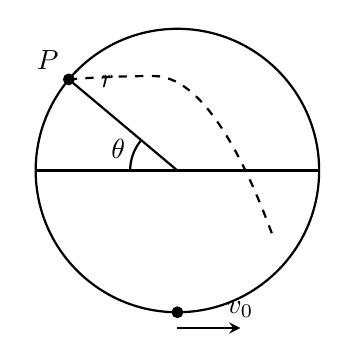
\begin{tikzpicture}[>=stealth, thick]
    \def\R{1.8}
    % Circle
    \draw (0,0) circle (\R);
    % Horizontal centerline
    \draw (-\R,0) -- (\R,0);
    % Point P and radius
    \draw (0,0) -- (140:\R);
    \node[above left] at (140:\R) {$P$};
    \filldraw[black] (140:\R) circle (0.06);
    \node[above right] at (140:0.8*\R) {$r$};
    % Angle theta
    \draw (-0.6,0) arc (180:140:0.6);
    \node at (160:0.8) {$\theta$};
    % Lowest point and velocity
    \filldraw[black] (0,-\R) circle (0.06);
    \draw[->] (0,-\R-0.2) -- (0.8,-\R-0.2) node[above] {$v_0$};
    % Dashed trajectory
    \draw[dashed] (140:\R) parabola bend (-0.3, 1.2) (1.2, -0.8);
\end{tikzpicture}
\end{center}
\end{exercise}
\begin{solution}

\end{solution}

\begin{exercise}\label{ex:3.14}
如图所示，一弹性绳悬挂一质量为 $m$ 的质点，从水平位置开始静止释放，此时弹性绳处于原长状态.
\begin{enumerate}
  \item[(a)] 从动力学及能量考虑，证明当伸长量 $\Delta \ell$ 与原长 $\ell$ 相比较小时，$\Delta \ell$ 可以表示为 $\Delta \ell = 3mg/k$；其中 $k$ 为弹性绳的劲度系数，注意 $k$ 越大，$\Delta \ell$ 越小，故近似 $\Delta \ell \ll \ell$ 越好；
  \item[(b)] 在上述情形中，试证明质点运动到最低点时的速度为 $v = \sqrt{2g(\ell - 3mg/2k)}$，该速度比悬线为非弹性时(相当于 $k=\infty$)的速度为小，给出该结果的物理解释.
\end{enumerate}
\begin{center}
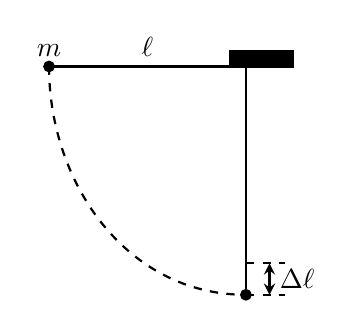
\begin{tikzpicture}[>=stealth, thick]
    \def\L{2.5}
    \def\dL{0.4}
    % Support
    \filldraw[black] (-0.2, 0) rectangle (0.6, 0.2);
    % Horizontal state
    \draw (0,0) -- (-\L, 0) node[midway, above] {$\ell$};
    \filldraw[black] (-\L, 0) circle (0.06) node[above] {$m$};
    
    % Vertical state
    \draw (0,0) -- (0, -\L-\dL);
    \filldraw[black] (0, -\L-\dL) circle (0.06);
    
    % Trajectory
    \draw[dashed] (-\L, 0) .. controls (-\L, -1.5) and (-1.5, -\L-\dL) .. (0, -\L-\dL);
    
    % Delta l label
    \draw[dashed] (0, -\L) -- (0.5, -\L);
    \draw[dashed] (0, -\L-\dL) -- (0.5, -\L-\dL);
    \draw[<->] (0.3, -\L) -- (0.3, -\L-\dL) node[right, midway] {$\Delta \ell$};
\end{tikzpicture}
\end{center}
\end{exercise}
\begin{solution}

\end{solution}
\chapter{第四章 引力}

1. $4.1 \times 10^{24}\text{kg}$

3. $185\text{m/s} ; 42.22\text{min}$

5. (a) $7.54 \times 10^3\text{m/s}$
(b) $5.84 \times 10^3\text{s}$
(c) $412\text{km}, 7.67 \times 10^3\text{m/s}, 5.56 \times 10^3\text{s}$
(d) $3.23 \times 10^{-3}\text{N}$
(e) 不守恒，变化 $2\%$

7. (a) $-\frac{Gm_{\oplus}m}{r}$
(b) $-\frac{Gm_{\oplus}(2m)}{r}$
(c) 下落到地球

9. 
$$\frac{p}{c^2} = \rho \frac{ \frac{1}{3}\left( 1 - \frac{2Mr^2G}{c^2R^3} \right)^{\frac{1}{2}} - \left( 1 - \frac{2MG}{c^2R} \right)^{\frac{1}{2}} }{ \left( 1 - \frac{2MG}{c^2R} \right)^{\frac{1}{2}} - \left( 1 - \frac{2Mr^2G}{c^2R^3} \right)^{\frac{1}{2}} }$$

11. $1.25$

13. $L = L_0 \exp\left(-\frac{\lambda}{m}t\right)$

15. (b) $0 = -\frac{Gm'm}{r^2} - mkr + \frac{L^2}{mr^3}$

17. $\varphi = \frac{k}{Eb}$

\begin{exercise}\label{ex:4.1}
一中子星半径为 $20 \ \mathrm{km}$，转速为 $1.0 \ \mathrm{/s}$. 它应有怎样的质量，表面物体才不会被甩出去？
\end{exercise}
\begin{solution}

\end{solution}

\begin{exercise}\label{ex:4.2}
轮船沿地球的赤道航行，该船上一弹簧秤下悬挂一物体. 设轮船的航行速度为 $v$，
\begin{enumerate}
  \item[(a)] 证明弹簧秤的读数为 $W_0 (1 \pm 2\omega v/g)$，其中 $W_0$ 是轮船静止时弹簧秤的读数，$\omega$ 是地球自转的角速度；
  \item[(b)] 解释该结果中出现的加减号的意义.
\end{enumerate}
\end{exercise}
\begin{solution}

\end{solution}

\begin{exercise}\label{ex:4.3}
巴黎和伦敦用一条直的地下铁道连结. 两城市间的火车在重力作用下运行. 试计算火车的最大速度以及从伦敦到巴黎旅行所用的时间. 两城市间的距离为 $300 \ \mathrm{km}$，地球半径为 $6400 \ \mathrm{km}$，忽略摩擦.
\end{exercise}
\begin{solution}

\end{solution}

\begin{exercise}\label{ex:4.4}
一半径为 $R$ 的铅制球体中有一位于球体表面与中心之间的空洞，如图所示. 设铅球未挖空前的质量为 $m'$，试求这一中空的铅球与球外一质量为 $m$ 的质点之间的引力；该质点位于铅球和空洞的连心线上，与铅球的中心距离为 $d$.
\begin{center}
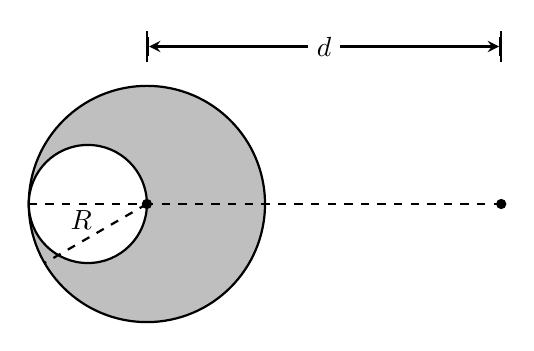
\begin{tikzpicture}[>=stealth, thick]
    \def\R{1.5}
    \def\d{4.5}
    
    % Big sphere with shading
    \draw[fill=gray!50] (0,0) circle (\R);
    
    % Cavity (white circle)
    \draw[fill=white] (-\R/2,0) circle (\R/2);
    
    % Dashed line passing through centers to the point
    \draw[dashed] (-\R,0) -- (\d,0);
    
    % Point mass
    \filldraw[black] (\d,0) circle (0.05);
    
    % Center of the large sphere
    \filldraw[black] (0,0) circle (0.05);
    
    % Radius R label
    \draw[dashed] (0,0) -- (210:\R);
    \node[above left, inner sep=1pt] at (210:\R/2) {$R$};
    
    % Dimension d
    \draw (0, \R+0.3) -- (0, \R+0.7);
    \draw (\d, \R+0.3) -- (\d, \R+0.7);
    \draw[|<->|] (0, \R+0.5) -- (\d, \R+0.5) node[midway, fill=white] {$d$};
\end{tikzpicture}
\end{center}
\end{exercise}
\begin{solution}

\end{solution}

\begin{exercise}\label{ex:4.5}
一质量为 $220 \ \mathrm{kg}$ 的卫星起初在距离地球表面 $640 \ \mathrm{km}$ 的轨道上运动，
\begin{enumerate}
  \item[(a)] 确定其速度；
  \item[(b)] 求其周期.
  \item[(c)] 由于多种原因，卫星每运行一周平均损失机械能 $1.4 \times 10^5 \ \mathrm{J}$. 作为近似，可认为卫星的轨道是一个半径逐渐变小的圆形，试确定卫星运行了 $1500$ 圈后与地球表面的距离、速度及周期；
  \item[(d)] 求平均阻力的大小.
  \item[(e)] 在此过程中角动量是否守恒？
\end{enumerate}
\end{exercise}
\begin{solution}

\end{solution}

\begin{exercise}\label{ex:4.6}
估算一下人通过跳跃就能脱离的小行星的半径有多大.
\end{exercise}
\begin{solution}

\end{solution}

\begin{exercise}\label{ex:4.7}
考虑两个具有相等质量 $m$ 的卫星 A 和 B，它们在相同的轨道 $r$ 上环绕地球运动，但是方向相反，故它们在某个时候将发生碰撞(如图). 
\begin{enumerate}
  \item[(a)] 用 $G$、$m_\oplus$、$m$ 和 $r$，求出碰撞前两个卫星及地球的总能量 $E_{\mathrm{A}} + E_{\mathrm{B}}$；
  \item[(b)] 若碰撞是非弹性的，并且碰撞碎片依旧聚集在一起(即质量变为 $2m$)，求碰撞后的总机械能；
  \item[(c)] 描述碰撞后碎片的运动.
\end{enumerate}
\begin{center}
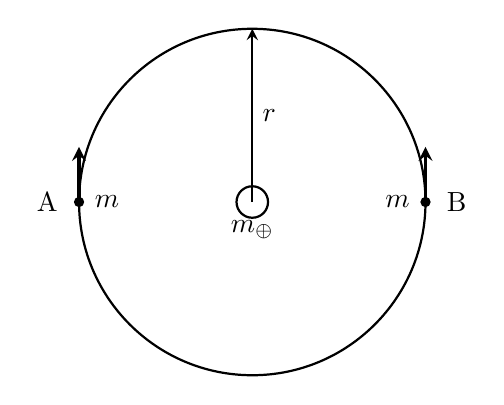
\begin{tikzpicture}[>=stealth, thick]
    \def\R{2.2}
    
    % Earth
    \draw (0,0) circle (0.2) node[below=3pt] {$m_\oplus$};
    
    % Orbit
    \draw (0,0) circle (\R);
    
    % Radius r
    \draw[->] (0,0) -- (0,\R);
    \node[right] at (0,\R/2) {$r$};
    
    % Satellite A
    \filldraw[black] (-\R,0) circle (0.05) node[left=4pt] {A} node[right=2pt] {$m$};
    \draw[->, very thick] (-\R,0) -- (-\R, 0.7);
    
    % Satellite B
    \filldraw[black] (\R,0) circle (0.05) node[right=4pt] {B} node[left=2pt] {$m$};
    \draw[->, very thick] (\R,0) -- (\R, 0.7);
\end{tikzpicture}
\end{center}
\end{exercise}
\begin{solution}

\end{solution}

\begin{exercise}\label{ex:4.8}
一火箭由地球(半径为 $R$)表面，以速度 $v = (v_r, v_\theta)$ 发射. 略去空气摩擦和地球转动(但用精确的重力场)，试求确定火箭所达到最大高度 $h$ 的方程. 将 $h/R$ 作为小量，求解该方程，并对 $v$ 是垂直向上的情形，给出结果.
\end{exercise}
\begin{solution}

\end{solution}

\begin{exercise}\label{ex:4.9}
试对均匀情形求解(4.3.12)式.
\end{exercise}
\begin{solution}

\end{solution}

\begin{exercise}\label{ex:4.10}
一质量为 $m$ 的质点沿着由 $x = x_0 \cos \omega_1 t$，$y = y_0 \sin \omega_2 t$ 所给定的轨道运动. 
\begin{enumerate}
  \item[(a)] 求质点所受作用力的 $x$ 分量和 $y$ 分量. 问在什么情况下，这个力是有心力？
  \item[(b)] 求势能(作为 $x$ 和 $y$ 的函数).
  \item[(c)] 确定该质点的动能. 证明质点的总能量守恒.
\end{enumerate}
\end{exercise}
\begin{solution}

\end{solution}

\begin{exercise}\label{ex:4.11}
环绕地球运动的卫星，其椭圆轨道的近地点距地球表面 $300 \ \mathrm{km}$，远地点距地球表面 $2000 \ \mathrm{km}$，试求卫星在轨道的近地点与远地点处的速率之比.
\end{exercise}
\begin{solution}

\end{solution}

\begin{exercise}\label{ex:4.12}
质量为 $m$ 的粒子受到大小为 $k/r^2$ 的引力作用，$k$ 为一常量. 在某个时刻如果粒子处于其封闭轨道的一个极端，此时与力心距离为 $a$，速度为 $\sqrt{k/2ma}$，
\begin{enumerate}
  \item[(a)] 求另一个极端的位置.
  \item[(b)] 粒子处于另一个极端时的速度是多少？
\end{enumerate}
\end{exercise}
\begin{solution}

\end{solution}

\begin{exercise}\label{ex:4.13}
一质量为 $m$ 的质点受到两个力的作用：一个是有心力 $\boldsymbol{F}_1 = f(r)\boldsymbol{e}_r$，另一个是摩擦力 $\boldsymbol{F}_2 = -\lambda \boldsymbol{v} \ (\lambda > 0)$，其中 $\boldsymbol{v}$ 是质点的速度. 若初始时刻该质点对 $r=0$ 点的角动量是 $\boldsymbol{L}_0$，求以后各时刻质点的角动量.
\end{exercise}
\begin{solution}

\end{solution}

\begin{exercise}\label{ex:4.14}
如果两体问题中的力是 $f(r) = -kr$，轨道将是怎样的？
\end{exercise}
\begin{solution}

\end{solution}

\begin{exercise}\label{ex:4.15}
考虑一个质量为 $m$ 的行星，环绕质量为 $m'$ 的恒星运动. 假定在恒星周围空间均匀分布有密度为 $\rho$ 的尘埃.
\begin{enumerate}
  \item[(a)] 证明尘埃的作用相当于增加一个附加的有心力，其大小为 $F' = -mkr$，式中
  $$k = \frac{4\pi}{3}\rho G$$
  $G$ 为引力常量. 忽略任何与尘埃碰撞的阻力.
  \item[(b)] 若行星在圆轨道上运动，角动量为 $L$，试利用 $L$、$G$、$m'$ 和 $k$ 来表示轨道半径 $r$ 所满足的方程. 不必求解方程.
\end{enumerate}
\end{exercise}
\begin{solution}

\end{solution}

\begin{exercise}\label{ex:4.16}
怎样根据轨道求力 $f(r)$？
\end{exercise}
\begin{solution}

\end{solution}

\begin{exercise}\label{ex:4.17}
从量纲分析导出(4.4.22)式.
\end{exercise}
\begin{solution}

\end{solution}

\begin{exercise}\label{ex:4.18}
一个球形物体以角速度 $\omega$ 转动.
\begin{enumerate}
  \item[(a)] 如果仅仅有引力阻碍球的离心撕裂，那么该球必须具有的最小密度是多少？利用这一点估计蟹状星云中转速为 $30 \ \mathrm{/s}$ 的脉冲星的最小密度.
  \item[(b)] 如果脉冲星的质量与太阳的质量相当，它的最大可能半径是多少？
\end{enumerate}
\end{exercise}
\begin{solution}

\end{solution}
\chapter{第五章 质点系动力学}

1. $0.42R$

3. $3\rho gx$

5. $v = \sqrt{g/k}$

7. (a) $0, 0, v_0$
(b) $-\frac{m' - m}{m + m'}v_0 ; 0; \frac{2m}{m + m'}v_0$

9. (a) $F = \frac{mv_0^2}{\ell}$
(b) $F = \frac{mv_0^2}{\ell}\left(\frac{\ell}{x}\right)^3$

13. (a) $v_C = [2g(d + h_2)]^{1/2}$
(b) $p_B = p_0 - \rho g(h_1 + d + h_2)$
(c) $10.3\text{m}$

\begin{exercise}\label{ex:5.1}
求均匀半圆板(半径为 $R$)的质心.
\end{exercise}
\begin{solution}

\end{solution}

\begin{exercise}\label{ex:5.2}
一质量为 $m$、半径为 $R$ 的小圆球位于相同质量、内半径为 $2R$ 的球壳内，球壳放在光滑桌面上，如图所示. 释放小球，任其下落，最后静止，求球壳移动了多远？
\begin{center}
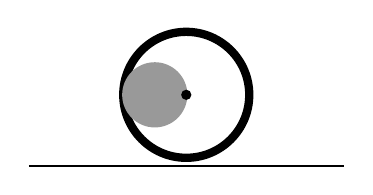
\begin{tikzpicture}[>=stealth, thick]
    \def\R{0.8}
    \def\r{0.4}
    % Table
    \draw (-2, -\R-0.1) -- (2, -\R-0.1);
    % Shell
    \draw[line width=3pt] (0,0) circle (\R);
    % Inner ball
    \filldraw[gray!80] (-0.4,0) circle (\r);
    \filldraw[black] (0,0) circle (0.05);
\end{tikzpicture}
\end{center}
\end{exercise}
\begin{solution}

\end{solution}

\begin{exercise}\label{ex:5.3}
将一质量为 $m$、长度为 $L$ 的柔软均匀链条的一端垂直地悬挂起来，其下端恰好接触到桌子的表面. 现将其上端突然释放，链条自由落至桌面并盘成一小堆，链条的每一节落至桌面时便立即静止，试用静止在桌面上的链条的质量来表示任一时刻桌面作用于链条上的力.
\end{exercise}
\begin{solution}

\end{solution}

\begin{exercise}\label{ex:5.4}
一火箭在均匀引力场中以恒定速率 $u$ 喷射气体而由静止升起. 假定气体排放率为 $\gamma m$，其中 $m$ 是火箭的瞬时质量，$\gamma$ 是常量；又假定使火箭减速的空气阻力是 $bv$，$b$ 为常量，$v$ 是火箭的速率. 求 $v$ (把它表示为时间的函数).
\\[1ex]
[提示：终极速度是 $m(\gamma u - g)/b$]
\end{exercise}
\begin{solution}

\end{solution}

\begin{exercise}\label{ex:5.5}
一雨滴的初始质量为 $m_0$，在重力的影响下，由静止开始降落. 假定此雨滴从云中得到质量，其质量的增长率正比于它的瞬时质量和瞬时速度的乘积：
$$ \frac{\mathrm{d}m}{\mathrm{d}t} = kmv $$
式中 $k$ 为常量. 试证明雨滴的速率实际上最后成为常量，并给出终极速率的表达式. 忽略空气的阻力.
\end{exercise}
\begin{solution}

\end{solution}

\begin{exercise}\label{ex:5.6}
如图所示，两物块在无摩擦的桌面上运动，其中 $k=1120 \ \mathrm{N/m}$，$m_1 = 2.0 \ \mathrm{kg}$，$v_1 = 10 \ \mathrm{m/s}$，$m_2 = 5.0 \ \mathrm{kg}$，$v_2 = 3.0 \ \mathrm{m/s}$. 求碰撞时弹簧的最大压缩量.
\begin{center}
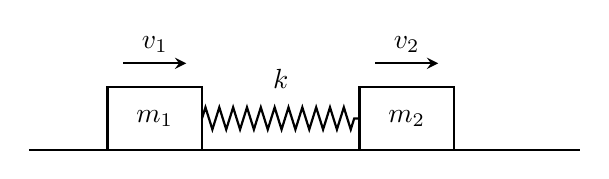
\begin{tikzpicture}[>=stealth, thick]
    % Ground
    \draw (-1, 0) -- (6, 0);
    
    % Block 1
    \draw[fill=white] (0,0) rectangle (1.2, 0.8);
    \node at (0.6, 0.4) {$m_1$};
    \draw[->] (0.2, 1.1) -- (1.0, 1.1) node[midway, above] {$v_1$};
    
    % Spring
    \draw[decorate, decoration={zigzag, segment length=5pt, amplitude=4pt}] (1.2, 0.4) -- (3.2, 0.4);
    \node at (2.2, 0.9) {$k$};
    
    % Block 2
    \draw[fill=white] (3.2, 0) rectangle (4.4, 0.8);
    \node at (3.8, 0.4) {$m_2$};
    \draw[->] (3.4, 1.1) -- (4.2, 1.1) node[midway, above] {$v_2$};
\end{tikzpicture}
\end{center}
\end{exercise}
\begin{solution}

\end{solution}

\begin{exercise}\label{ex:5.7}
如图所示，右侧的两个小球起初静止并略微分离，左侧有一小球以速度 $v_0$ 入射，假设碰撞是弹性正碰：
\begin{enumerate}
  \item[(a)] 若 $m'=m$，说明整个过程中有两次碰撞并求各球最后的速度；
  \item[(b)] 若 $m'>m$，说明有三次碰撞并求各球最后的速度.
\end{enumerate}
\begin{center}
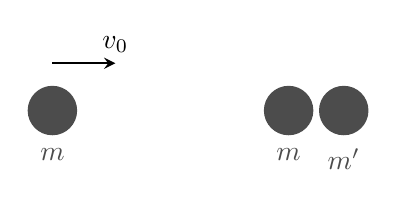
\begin{tikzpicture}[>=stealth, thick]
    \filldraw[black!70] (0,0) circle (0.3) node[below=10pt] {$m$};
    \draw[->] (0, 0.6) -- (0.8, 0.6) node[above] {$v_0$};
    
    \filldraw[black!70] (3,0) circle (0.3) node[below=10pt] {$m$};
    \filldraw[black!70] (3.7,0) circle (0.3) node[below=10pt] {$m'$};
\end{tikzpicture}
\end{center}
\end{exercise}
\begin{solution}

\end{solution}

\begin{exercise}\label{ex:5.8}
慢中子与静止重水中的氘核发生弹性碰撞，若中子的散射角为 $90^\circ$，试证明其动能将损失 $2/3$ 并传递给了氘核.
\end{exercise}
\begin{solution}

\end{solution}

\begin{exercise}\label{ex:5.9}
如图所示，一质量为 $m$ 的球在两个壁面间以速度 $v_0$ 来回弹跳，碰撞是完全弹性的. 略去重力不计，
\begin{enumerate}
  \item[(a)] 求每个壁所受到的平均作用力 $F$.
  \item[(b)] 如果一个表面以 $v \ll v_0$ 的速率缓慢地移向另一表面，则回跳频率由于碰撞间的距离减小以及球从运动的表面碰回时，球的速率增大而增加. 求出用表面间的距离 $x$ 来表示的力 $F$.
  \item[(c)] 证明：把表面从距离 $\ell$ 推近到距离 $x$ 时所作的功等于球的动能的增加. （这个问题说明了当气体压缩时温度升高的机制.）
\end{enumerate}
\begin{center}
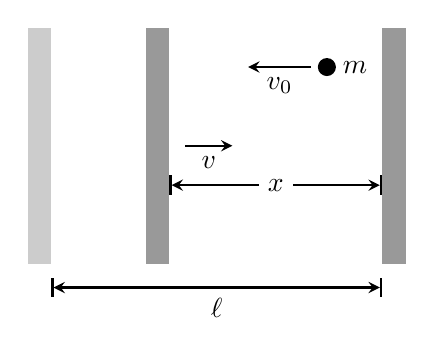
\begin{tikzpicture}[>=stealth, thick]
    % Right Wall
    \fill[gray!80] (4.5,0) rectangle (4.8, 3);
    
    % Left Wall (Moving)
    \fill[gray!80] (1.5,0) rectangle (1.8, 3);
    \draw[->] (2.0, 1.5) -- (2.6, 1.5) node[midway, below] {$v$};
    
    % Left Wall (Initial position dashed)
    \fill[gray!40] (0,0) rectangle (0.3, 3);
    
    % Distance l
    \draw[|<->|] (0.3, -0.3) -- (4.5, -0.3) node[midway, below] {$\ell$};
    
    % Distance x
    \draw[|<->|] (1.8, 1.0) -- (4.5, 1.0) node[midway, fill=white] {$x$};
    
    % Ball
    \filldraw[black] (3.8, 2.5) circle (0.1) node[right=2pt] {$m$};
    \draw[->] (3.6, 2.5) -- (2.8, 2.5) node[midway, below] {$v_0$};
\end{tikzpicture}
\end{center}
\end{exercise}
\begin{solution}

\end{solution}

\begin{exercise}\label{ex:5.10}
用能量为 $E_0$ 的氢原子核去轰击一个薄的锂靶. 锂原子核原来静止于靶内，但基本上是不受束缚的. 当氢核进入一锂核，就能产生反应，复合核分裂为一个硼核和一个中子. 碰撞是非弹性的，而最后的动能比 $E_0$ 少了 $2.8 \ \mathrm{MeV}$. 粒子的相对质量是：氢为 4，锂为 7，硼为 10，中子为 1. 这个反应可写为
$$ ^7\mathrm{Li} + ^4\mathrm{He} \rightarrow ^{10}\mathrm{B} + \mathrm{n} - 2.8 \ \mathrm{MeV} $$
\begin{enumerate}
  \item[(a)] 可以产生中子所需的 $E_0$ 的最小值 $E_{0\min}$ 是多少？在此阈限上，中子能量是多少？
  \item[(b)] 证明：如果入射能量落在 $E_{0\min} < E_0 < E_{0\min} + 0.27 \ \mathrm{MeV}$ 范围内时，则向前抛出的中子的能量并不都一样，但必定是两个可能的能量值的一个. (在质心坐标系中看这个反应，即可得出这两个能量的来源.)
\end{enumerate}
\end{exercise}
\begin{solution}

\end{solution}

\begin{exercise}\label{ex:5.11}
质量为 $m_1$ 的粒子与起初静止的质量为 $m_2$ 的粒子发生弹性碰撞，证明：
\begin{enumerate}
  \item[(a)] $m_1$ 的最大散射角 $\theta_m$ 由下式确定：$\cos^2 \theta_m = 1 - m_2^2/m_1^2$，故当 $m_1 > m_2$ 时，有 $0 \le \theta_m \le \pi/2$；
  \item[(b)] 当 $m_1 = m_2$ 时，有 $\theta_1 + \theta_2 = \pi/2$，$\theta_1$ 和 $\theta_2$ 分别是 $m_1$ 和 $m_2$ 的散射角；
  \item[(c)] 当 $m_1 < m_2$ 时，$\theta_1$ 可以取 $0$ 到 $\pi$ 之间的所有值.
\end{enumerate}
\end{exercise}
\begin{solution}

\end{solution}

\begin{exercise}\label{ex:5.12}
如图，密度为 $\rho$ 的流体以速度 $v_1$ 流经一横截面积为 $a_1$ 的较窄的区域，然后在某处突然到达横截面积为 $a_2$ 的较宽的区域，并与周围的液体混合后一同以速度 $v_2$ 继续流动.
\begin{enumerate}
  \item[(a)] 若不考虑混合过程的细节，用动量的概念证明由于混合而引起压强的增加近似为
  $$ p_2 - p_1 = \rho v_2 (v_1 - v_2) $$
  \item[(b)] 根据伯努利方程，证明对于逐渐变宽的管道，其压力的增加应为
  $$ p_2 - p_1 = \frac{1}{2} \rho (v_1^2 - v_2^2) $$
  \item[(c)] 计算突变情形下压力的损失. 你能与动力学中的弹性或非弹性碰撞作一类比吗？
\end{enumerate}
\begin{center}
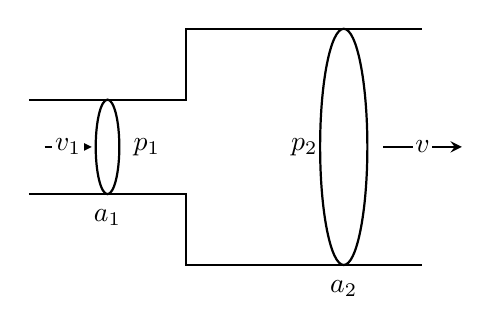
\begin{tikzpicture}[>=stealth, thick]
    % Pipe lines
    \draw (0, 0.6) -- (2, 0.6) -- (2, 1.5) -- (5, 1.5);
    \draw (0, -0.6) -- (2, -0.6) -- (2, -1.5) -- (5, -1.5);
    
    % Cross sections
    \draw (1, 0) ellipse (0.15 and 0.6);
    \node at (1, -0.9) {$a_1$};
    \node at (1.5, 0) {$p_1$};
    
    \draw (4, 0) ellipse (0.3 and 1.5);
    \node at (4, -1.8) {$a_2$};
    \node at (3.5, 0) {$p_2$};
    
    % Flow arrows
    \draw[->] (0.2, 0) -- (0.8, 0) node[midway, fill=white, inner sep=1pt] {$v_1$};
    \draw[->] (4.5, 0) -- (5.5, 0) node[midway, fill=white, inner sep=1pt] {$v$};
\end{tikzpicture}
\end{center}
\end{exercise}
\begin{solution}

\end{solution}

\begin{exercise}\label{ex:5.13}
利用虹吸现象，可以取出容器中液体而无须倾斜容器. 如图所示，首先要将其中的管道注满液体，而液体一旦开始流动，则该过程将一直持续至容器中的液面低于管道的开口 $A$ 端. 设液体的密度为 $\rho$，并忽略其黏性. 
\begin{enumerate}
  \item[(a)] 从管道的开口 $C$ 处流出的液体的速率是多少？
  \item[(b)] 在最高点 $B$ 处液体的压强是多少？
  \item[(c)] 使虹吸现象能够发生的 $h_1$ 的最大高度是多少？
\end{enumerate}
\begin{center}
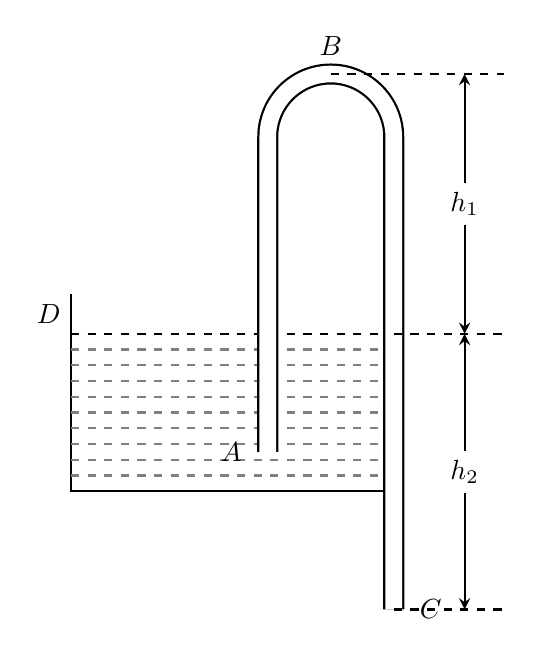
\begin{tikzpicture}[>=stealth, thick]
    % Container
    \draw (-2, 2.5) -- (-2, 0) -- (2, 0) -- (2, 2.5);
    
    % Liquid lines (representing fluid)
    \foreach \y in {0.2, 0.4, 0.6, 0.8, 1.0, 1.2, 1.4, 1.6, 1.8} {
        \draw[dashed, gray] (-2, \y) -- (2, \y);
    }
    
    % Surface D
    \draw[dashed] (-2, 2.0) -- (2, 2.0);
    \node[above left] at (-2, 2.0) {$D$};
    
    % Siphon Tube
    \draw[double=white, double distance=6pt] (0.5, 0.5) -- (0.5, 4.5) arc (180:0:0.8) -- (2.1, -1.5);
    \node[left] at (0.3, 0.5) {$A$};
    \node[above] at (1.3, 5.4) {$B$};
    \node[right] at (2.3, -1.5) {$C$};
    
    % Heights
    \draw[dashed] (2.1, 2.0) -- (3.5, 2.0);
    \draw[dashed] (1.3, 5.3) -- (3.5, 5.3);
    \draw[dashed] (2.1, -1.5) -- (3.5, -1.5);
    
    \draw[<->] (3.0, 2.0) -- (3.0, 5.3) node[midway, fill=white] {$h_1$};
    \draw[<->] (3.0, 2.0) -- (3.0, -1.5) node[midway, fill=white] {$h_2$};
\end{tikzpicture}
\end{center}
\end{exercise}
\begin{solution}

\end{solution}
\chapter{第六章 刚体动力学}

1. $\frac{1}{3}m(a^2 + b^2)$

7. $\frac{55}{128} \frac{v_0^2}{\mu g}$

11. $2.2\text{m}$

\begin{exercise}\label{ex:6.1}
质量为 $m$ 的 $a \times b$ 均匀矩形薄板绕通过一个顶角垂直板面的轴转动，求其转动惯量.
\end{exercise}
\begin{solution}

\end{solution}

\begin{exercise}\label{ex:6.2}
竖直米尺从静止开始倒下时，下端不滑动，求上端落地时的速度.
\end{exercise}
\begin{solution}

\end{solution}

\begin{exercise}\label{ex:6.3}
总长度为 $\ell$ 的柔软的带子先是被紧紧地缠在一团，然后置于倾角为 $\theta$ 的斜面上让其滚下并自动解开，其上端固定(如图所示)，证明这团带子要完全解开所需时间为 $t = \sqrt{3\ell / g\sin\theta}$.
\begin{center}
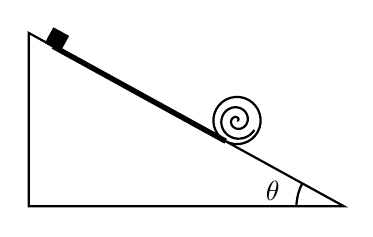
\begin{tikzpicture}[>=stealth, thick]
    \def\W{4}
    \def\H{2.2}
    % Triangle
    \draw (0,\H) -- (0,0) -- (\W,0) -- cycle;
    
    % Angle theta
    \draw (\W-0.6, 0) arc (180:151.2:0.6);
    \node at (\W-0.9, 0.2) {$\theta$};
    
    % Tape on incline
    \begin{scope}[shift={(2.5, 0.825)}, rotate=-28.8]
        % Roll
        \draw[fill=white] (0, 0.3) circle (0.3);
        \draw[domain=0:4*pi, variable=\t, samples=100] plot ({0.02*\t*cos(\t r)}, {0.3 + 0.02*\t*sin(\t r)});
        % Unrolled tape
        \draw (-2.5, 0.02) -- (0, 0.02);
        \draw (-2.5, -0.02) -- (0, -0.02);
        % Fixed end
        \filldraw[black] (-2.6, 0) rectangle (-2.4, 0.2);
    \end{scope}
\end{tikzpicture}
\end{center}
\end{exercise}
\begin{solution}

\end{solution}

\begin{exercise}\label{ex:6.4}
如图，一质量为 $m'$、半径为 $R$ 的均匀球壳可以绕其对称轴无摩擦地转动，有一轻质细绳缠绕在球壳的水平方向的大圆上并通过半径为 $r$、转动惯量为 $I$ 的滑轮悬挂一重物，试求该重物由静止开始下落高度 $h$ 后的速度.
\begin{center}
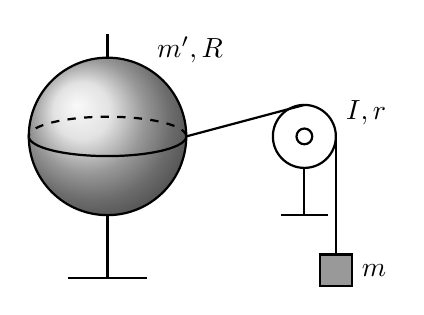
\begin{tikzpicture}[>=stealth, thick]
    % Stand for sphere
    \draw (-0.5, -1.8) -- (0.5, -1.8);
    \draw (0, -1.8) -- (0, -1);
    \draw (0, 1) -- (0, 1.3);
    
    % Sphere
    \shade[ball color=gray!30] (0,0) circle (1);
    \draw (0,0) circle (1);
    \draw (-1,0) arc (180:360:1 and 0.25);
    \draw[dashed] (1,0) arc (0:180:1 and 0.25);
    \node[above right] at (0.5, 0.8) {$m', R$};
    
    % Stand for pulley
    \draw (2.5, 0) -- (2.5, -1);
    \draw (2.2, -1) -- (2.8, -1);
    
    % Pulley
    \draw[fill=white] (2.5, 0) circle (0.4);
    \draw[fill=white] (2.5, 0) circle (0.1);
    \node[right] at (2.9, 0.3) {$I, r$};
    
    % String
    \draw (1,0) -- (2.5, 0.4);
    \draw (2.9, 0) -- (2.9, -1.5);
    
    % Mass
    \draw[fill=gray!80] (2.7, -1.5) rectangle (3.1, -1.9);
    \node[right] at (3.1, -1.7) {$m$};
\end{tikzpicture}
\end{center}
\end{exercise}
\begin{solution}

\end{solution}

\begin{exercise}\label{ex:6.5}
如图，一块长度为 $2L$ 的木板斜靠在墙上无摩擦的下滑. 证明：当木板高度为原来高度的 $2/3$ 时，它的顶端便与墙脱离接触.
\begin{center}
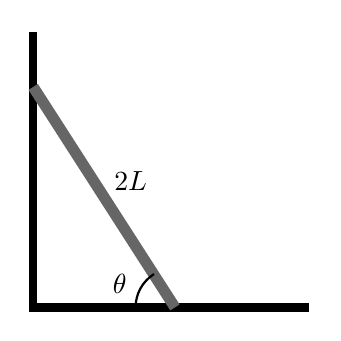
\begin{tikzpicture}[>=stealth, thick]
    % Wall and Floor
    \draw[line width=3pt] (0, 3.5) -- (0,0) -- (3.5, 0);
    
    % Plank
    \draw[line width=4pt, gray!80!black] (0, 2.8) -- (1.8, 0);
    
    % Labels
    \node[right] at (0.9, 1.6) {$2L$};
    \draw (1.3, 0) arc (180:122:0.5);
    \node at (1.1, 0.3) {$\theta$};
\end{tikzpicture}
\end{center}
\end{exercise}
\begin{solution}

\end{solution}

\begin{exercise}\label{ex:6.6}
一小球在一个大的半球内无滑动地滚下，半球的对称轴是垂直的，小球从上边由静止开始滚动. 
\begin{enumerate}
  \item[(a)] 小球到达半球的底部时动能是多少？其中有多少是转动动能？多少是平动动能？
  \item[(b)] 此时小球作用于半球的正压力是多少？
\end{enumerate}
设小球的半径是 $r$，半球的半径是 $R$，小球的质量是 $m$.
\end{exercise}
\begin{solution}

\end{solution}

\begin{exercise}\label{ex:6.7}
如图，弹子球被球杆所击，力的作用线水平并且通过弹子球的球心，球的初速度是 $v_0$. 设弹子球的半径是 $R$，质量是 $m$，球与桌面之间的摩擦系数为 $\mu$，问弹子球在停止滑动前能运动多远？
\begin{center}
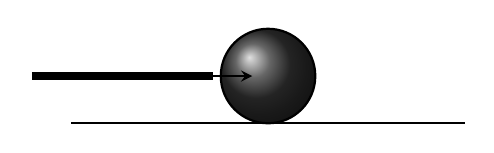
\begin{tikzpicture}[>=stealth, thick]
    % Table
    \draw (-2.5, 0) -- (2.5, 0);
    
    % Ball
    \shade[ball color=black!80] (0, 0.6) circle (0.6);
    \draw (0, 0.6) circle (0.6);
    
    % Cue stick
    \draw[line width=3pt] (-3, 0.6) -- (-0.7, 0.6);
    \draw[->] (-0.7, 0.6) -- (-0.2, 0.6);
\end{tikzpicture}
\end{center}
\end{exercise}
\begin{solution}

\end{solution}

\begin{exercise}\label{ex:6.8}
一根质量可以忽略的刚性杆，长度为 $L$，连接着质量各为 $m$ 的两个质点，放在无摩擦的桌面上. 另一个质量为 $m$ 的质点，以速度 $v_0$ 撞击上述系统，如图所示. 碰撞后，该质点直接返回. 假定机械能守恒，求碰撞后系统绕质心的角速度.
\begin{center}
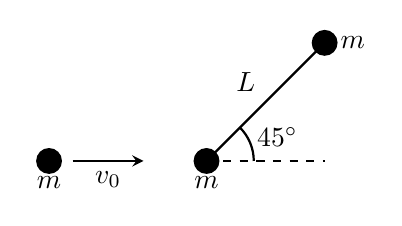
\begin{tikzpicture}[>=stealth, thick]
    % Incoming mass
    \filldraw[black] (-2, 0) circle (0.15) node[below=2pt] {$m$};
    \draw[->] (-1.7, 0) -- (-0.8, 0) node[midway, below] {$v_0$};
    
    % Rod system
    \filldraw[black] (0, 0) circle (0.15) node[below=2pt] {$m$};
    \draw (0, 0) -- (1.5, 1.5) node[midway, above left] {$L$};
    \filldraw[black] (1.5, 1.5) circle (0.15) node[right=2pt] {$m$};
    
    % Angle
    \draw[dashed] (0, 0) -- (1.5, 0);
    \draw (0.6, 0) arc (0:45:0.6);
    \node at (0.9, 0.3) {$45^\circ$};
\end{tikzpicture}
\end{center}
\end{exercise}
\begin{solution}

\end{solution}

\begin{exercise}\label{ex:6.9}
四块质量相同长度均为 $\ell$ 的砖块按图示重叠放置，每一块都相对于下面的一块伸出一部分. 试证明，若要使它们维持平衡，则应按如下方式放置：
\begin{enumerate}
  \item[(a)] 最上面的砖块相对于下面一砖块伸出 $\ell/2$；
  \item[(b)] 第二块砖相对于第三块砖伸出 $\ell/4$；
  \item[(c)] 第三块砖相对于最下面的砖块伸出 $\ell/6$.
\end{enumerate}
叙述这样做的力学原理.
\begin{center}
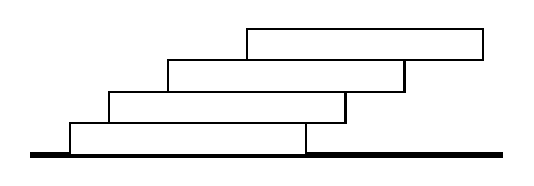
\begin{tikzpicture}[>=stealth, thick]
    % Ground
    \draw[line width=2pt] (0, 0) -- (6, 0);
    
    % Bricks
    \draw[fill=white] (0.5, 0) rectangle (3.5, 0.4);
    \draw[fill=white] (1.0, 0.4) rectangle (4.0, 0.8);
    \draw[fill=white] (1.75, 0.8) rectangle (4.75, 1.2);
    \draw[fill=white] (2.75, 1.2) rectangle (5.75, 1.6);
\end{tikzpicture}
\end{center}
\end{exercise}
\begin{solution}

\end{solution}

\begin{exercise}\label{ex:6.10}
关于砖块的堆置有下述较为有名的问题. 均匀的砖块一块叠一块地放置，以求到达最大伸展量. 为此使最上面砖块的重心恰好垂直地位于其下面砖块的边缘上，最上面两块砖的合重心的位置恰位于第三块砖的边缘上，依此类推. 
\begin{enumerate}
  \item[(a)] 证明这个做法确实可以获得最大伸展量. 
  \item[(b)] 证明，若该过程一直持续进行下去，我们可以获得任意想要的伸展量. 
  \item[(c)] 现在设想换一种方法堆置 $n$ 块砖块，即每一块砖相对于其下相邻的砖伸出 $1/n$，砖的长度是 $\ell$，那么，在砖块倒塌之前，我们最多能放置的砖块的数目 $n_{\max}$ 是多少？试就 $n=1, n=2, n=\infty$ 加以检验.
\end{enumerate}
\end{exercise}
\begin{solution}

\end{solution}

\begin{exercise}\label{ex:6.11}
重量为 $W$ 的非均匀杆被两根轻绳水平地悬挂在两面直立的墙之间并处于静止状态(如图)，绳与墙的夹角分别为 $\theta = 36.9^\circ$ 和 $\varphi = 53.1^\circ$，若杆的长度 $\ell$ 为 $61 \ \mathrm{m}$，试计算杆的重心距其左端的距离.
\begin{center}
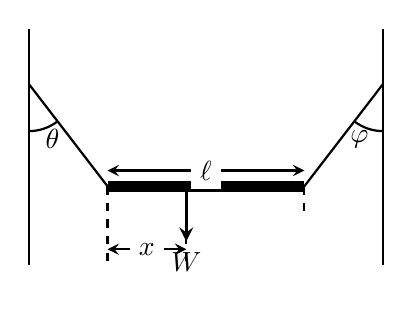
\begin{tikzpicture}[>=stealth, thick]
    % Walls
    \draw (0, 2.5) -- (0, -0.5);
    \draw (4.5, 2.5) -- (4.5, -0.5);
    
    % Rod
    \draw[line width=4pt] (1.0, 0.5) -- (3.5, 0.5);
    
    % Strings
    \draw (0, 1.8) -- (1.0, 0.5);
    \draw (4.5, 1.8) -- (3.5, 0.5);
    
    % Angles
    \draw (0, 1.2) arc (270:307.5:0.6);
    \node at (0.3, 1.1) {$\theta$};
    
    \draw (4.5, 1.2) arc (270:232.5:0.6);
    \node at (4.2, 1.1) {$\varphi$};
    
    % Dimensions and forces
    \draw[dashed] (1.0, 0.5) -- (1.0, -0.5);
    \draw[dashed] (3.5, 0.5) -- (3.5, 0.1);
    \draw[<->] (1.0, 0.7) -- (3.5, 0.7) node[midway, fill=white] {$\ell$};
    
    \draw[dashed] (2.0, 0.5) -- (2.0, -0.5);
    \draw[->, very thick] (2.0, 0.5) -- (2.0, -0.2) node[below] {$W$};
    
    \draw[<->] (1.0, -0.3) -- (2.0, -0.3) node[midway, fill=white] {$x$};
\end{tikzpicture}
\end{center}
\end{exercise}
\begin{solution}

\end{solution}

\begin{exercise}\label{ex:6.12}
半径为 $R$ 的半球形碗置于粗糙桌面上，碗内装有沙子，质心高 $h$. 讨论系统的平衡性质和条件.
\end{exercise}
\begin{solution}

\end{solution}
\chapter{第七章 振动}

3. $\omega = \sqrt{5g/7R}$

7. $6$

\begin{exercise}\label{ex:7.1}
证明：
\begin{enumerate}
  \item[(a)] 对于简谐运动，在一个周期中势能的平均值和动能的平均值均为 $kA^2/4$ (其中 $k$ 是回复力的系数，$A$ 是振幅.)；
  \item[(b)] 若考虑对空间平均，则势能的平均值等于 $kA^2/6$，动能的平均值等于 $kA^2/3$.
  \item[(c)] 解释上述差异的物理意义.
\end{enumerate}
\end{exercise}
\begin{solution}

\end{solution}

\begin{exercise}\label{ex:7.2}
常用的一个势能函数是伦纳德-琼斯势：
$$U = 4\varepsilon \left[ \left(\frac{\sigma}{r}\right)^{12} - \left(\frac{\sigma}{r}\right)^6 \right]$$
\begin{enumerate}
  \item[(a)] 求势能最小处的半径及势阱的深度.
  \item[(b)] 若质量均为 $m$ 的两个相同的原子，以林纳德-琼斯势相互作用而束缚在一起，并在平衡位置作微小振动. 求其振动频率.
\end{enumerate}
\end{exercise}
\begin{solution}

\end{solution}

\begin{exercise}\label{ex:7.3}
一个半径为 $r$ 的大理石小球，在半径为 $R$ 的浅碟子中来回滚动. 已知 $R \gg r$，求小球作小振动的频率.
\end{exercise}
\begin{solution}

\end{solution}

\begin{exercise}\label{ex:7.4}
如图，将一质量为 $m$ 的圆柱形刚体与水平放置的轻质弹簧连接在一起，使该刚体可以沿水平面无摩擦的滚动，弹簧的劲度系数为 $3.0 \ \mathrm{N/m}$. 设圆柱从偏离平衡位置 $0.25 \ \mathrm{m}$ 处由静止释放，计算当圆柱滚动到平衡位置时的
\begin{enumerate}
  \item[(a)] 平动动能、
  \item[(b)] 滚动动能.
  \item[(c)] 证明在这些情形下，圆柱的质心作简谐运动，其周期是 $T = 2\pi\sqrt{3m/2k}$.
\end{enumerate}
\begin{center}
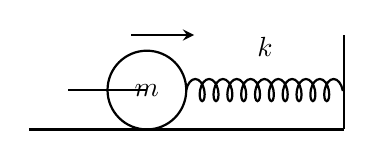
\begin{tikzpicture}[>=stealth, thick]
    % Ground
    \draw (-1.5, 0) -- (2.5, 0);
    % Wall
    \draw (2.5, 0) -- (2.5, 1.2);
    % Cylinder
    \draw (0, 0.5) circle (0.5);
    \node at (0, 0.5) {$m$};
    % Horizontal line through center
    \draw (-1, 0.5) -- (0, 0.5);
    % Spring
    \draw[decorate, decoration={coil, segment length=5pt, amplitude=4pt}] (0.5, 0.5) -- (2.5, 0.5);
    \node[above] at (1.5, 0.8) {$k$};
    % Arrow
    \draw[->] (-0.2, 1.2) -- (0.6, 1.2);
\end{tikzpicture}
\end{center}
\end{exercise}
\begin{solution}

\end{solution}

\begin{exercise}\label{ex:7.5}
若弹簧的质量 $m_s$ 不可忽略，但远比悬挂其下的物体质量 $m$ 为小，试证明其振动周期为
$$T = 2\pi\sqrt{(m + m_s/3)/k}$$
\end{exercise}
\begin{solution}

\end{solution}

\begin{exercise}\label{ex:7.6}
两个质量均为 $m$ 的质点 1 和 2，连接于 3 个相同的弹簧上. 弹簧的质量可以忽略，劲度系数为 $k$. 忽略重力. 两质点间连接一质量可忽略的阻尼减震器，如图所示. 阻尼减震器的阻力为 $bv$，这里 $v$ 是它两端的相对速度. 令 $x_1$ 与 $x_2$ 为两质点离开其平衡位置的位移.
\begin{enumerate}
  \item[(a)] 求每个质点的运动方程.
  \item[(b)] 证明运动方程可以利用新的变量 $y_1 = x_1 + x_2$ 和 $y_2 = x_1 - x_2$ 来求解.
  \item[(c)] 证明：如果两质点原来是静止的，后给质点 1 以速度 $v_0$，则在足够长的时间以后，两个质点的运动为
  $$x_1 = x_2 = \frac{v_0}{2\omega} \sin \omega t$$
  并计算出 $\omega$.
\end{enumerate}
\begin{center}
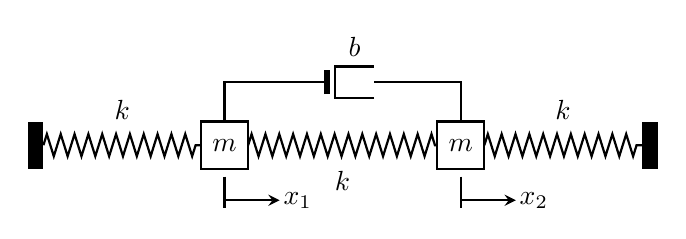
\begin{tikzpicture}[>=stealth, thick]
    % Walls
    \fill[black] (-4, -0.3) rectangle (-3.8, 0.3);
    \fill[black] (3.8, -0.3) rectangle (4, 0.3);
    
    % Masses
    \draw[fill=white] (-1.8, -0.3) rectangle (-1.2, 0.3);
    \node at (-1.5, 0) {$m$};
    \draw[fill=white] (1.2, -0.3) rectangle (1.8, 0.3);
    \node at (1.5, 0) {$m$};
    
    % Springs
    \draw[decorate, decoration={zigzag, segment length=5pt, amplitude=4pt}] (-3.8, 0) -- (-1.8, 0);
    \node[above] at (-2.8, 0.2) {$k$};
    \draw[decorate, decoration={zigzag, segment length=5pt, amplitude=4pt}] (-1.2, 0) -- (1.2, 0);
    \node[below] at (0, -0.2) {$k$};
    \draw[decorate, decoration={zigzag, segment length=5pt, amplitude=4pt}] (1.8, 0) -- (3.8, 0);
    \node[above] at (2.8, 0.2) {$k$};
    
    % Damper Connectors
    \draw (-1.5, 0.3) -- (-1.5, 0.8) -- (-0.2, 0.8);
    \draw (1.5, 0.3) -- (1.5, 0.8) -- (0.4, 0.8);
    
    % Damper Cylinder
    \draw (0.4, 0.6) -- (-0.1, 0.6) -- (-0.1, 1.0) -- (0.4, 1.0);
    
    % Damper Piston
    \draw[line width=2pt] (-0.2, 0.65) -- (-0.2, 0.95);
    \node[above] at (0.15, 1.0) {$b$};
    
    % x1, x2 Coordinates
    \draw (-1.5, -0.4) -- (-1.5, -0.8);
    \draw[->] (-1.5, -0.7) -- (-0.8, -0.7) node[right, inner sep=1pt] {$x_1$};
    
    \draw (1.5, -0.4) -- (1.5, -0.8);
    \draw[->] (1.5, -0.7) -- (2.2, -0.7) node[right, inner sep=1pt] {$x_2$};
\end{tikzpicture}
\end{center}
\end{exercise}
\begin{solution}

\end{solution}

\begin{exercise}\label{ex:7.7}
如图，立方块的质量为 $1.5 \ \mathrm{kg}$，弹簧的劲度系数为 $8.0 \ \mathrm{N/m}$. 将方块向下拉 $12 \ \mathrm{cm}$ 后释放，运动过程中液体对浸于其中的板有阻尼，设为 $-b \, \mathrm{d}x/\mathrm{d}t$，这里 $b = 0.23 \ \mathrm{kg/s}$，试计算从开始到振幅变为最初的 $1/3$ 时方块振动的次数.
\begin{center}
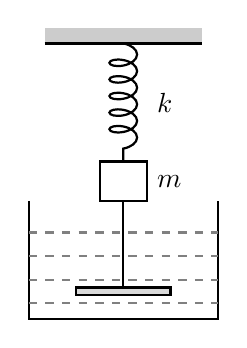
\begin{tikzpicture}[>=stealth, thick]
    % Ceiling
    \fill[gray!40] (-1, 3) rectangle (1, 3.2);
    \draw (-1, 3) -- (1, 3);
    
    % Spring
    \draw[decorate, decoration={coil, segment length=6pt, amplitude=5pt}] (0, 3) -- (0, 1.5);
    \node[right] at (0.3, 2.25) {$k$};
    
    % Mass
    \draw[fill=white] (-0.3, 1.0) rectangle (0.3, 1.5);
    \node[right] at (0.3, 1.25) {$m$};
    
    % Rod and Plate
    \draw (0, 1.0) -- (0, -0.2);
    \draw[fill=gray!30] (-0.6, -0.2) rectangle (0.6, -0.1);
    
    % Container
    \draw (-1.2, 1.0) -- (-1.2, -0.5) -- (1.2, -0.5) -- (1.2, 1.0);
    
    % Liquid lines
    \draw[dashed, gray] (-1.2, 0.6) -- (1.2, 0.6);
    \draw[dashed, gray] (-1.2, 0.3) -- (1.2, 0.3);
    \draw[dashed, gray] (-1.2, 0.0) -- (1.2, 0.0);
    \draw[dashed, gray] (-1.2, -0.3) -- (1.2, -0.3);
\end{tikzpicture}
\end{center}
\end{exercise}
\begin{solution}

\end{solution}

\begin{exercise}\label{ex:7.8}
证明对于强迫阻尼振动，外力的平均功率等于阻尼力耗散的功率.
\end{exercise}
\begin{solution}

\end{solution}
\chapter{第八章 波}

1. $v_0$

3. $8.3 \times 10^{10}\text{kg/(m}\cdot\text{s}^2\text{)}$

5. $(60 \pm 1)\text{/m}$

13. $I \propto \frac{1}{\rho} ; \quad A \propto \frac{1}{\sqrt{\rho}}$

15. (a) $u = 5.0 \cos \left( 4.0t \mp 0.05x + \frac{\pi}{2} - \begin{matrix} 0.5 \\ 1.5 \end{matrix} \right)$
(b) $0.26\text{N}$

19. 不可

21. $2.6 \times 10^8\text{m/s}$

\begin{exercise}\label{ex:8.1}
一均匀的圆环在无重力的空间顺时针转动，其切向线速度为 $v_0$. 求沿环传播的波的速度.
\end{exercise}
\begin{solution}

\end{solution}

\begin{exercise}\label{ex:8.2}
质量为 $m$、长度为 $L$ 的均匀绳垂直悬挂在天花板上，
\begin{enumerate}
  \item[(a)] 证明绳中各点横波的速度可以表示为 $v = \sqrt{gy}$，其中 $y$ 为相应点到绳下端的距离.
  \item[(b)] 证明横波从绳的上端传至绳的下端所用时间为 $t = 2\sqrt{L/g}$.
  \item[(c)] 绳的质量是否影响上述结果？
\end{enumerate}
\end{exercise}
\begin{solution}

\end{solution}

\begin{exercise}\label{ex:8.3}
地震造成的纵扰动 $15 \ \mathrm{min}$ 传播了 $5000 \ \mathrm{km}$，试估计传播扰动的岩石的杨氏模量. 假定岩石的平均密度是 $2700 \ \mathrm{kg/m^3}$.
\end{exercise}
\begin{solution}

\end{solution}

\begin{exercise}\label{ex:8.4}
用等温压缩率而不是绝热压缩率来计算声速，会造成多大的百分误差？
\end{exercise}
\begin{solution}

\end{solution}

\begin{exercise}\label{ex:8.5}
一块石头扔到水塘中，产生的行波群约 $1 \ \mathrm{m}$ 长. 波群中波的波长约 $0.1 \ \mathrm{m}$. 估算代表波群的波矢谱的范围.
\end{exercise}
\begin{solution}

\end{solution}

\begin{exercise}\label{ex:8.6}
一个系统具有色散关系 $\omega = a k^\beta$. 证明对所有频率有 $v_g = \beta v_p$.
\end{exercise}
\begin{solution}

\end{solution}

\begin{exercise}\label{ex:8.7}
一个波群是由平均波长为 $\lambda$ 的谐波叠加而成. 如果 $v_p(\lambda)$ 是波长为 $\lambda$ 的波的相速，证明群速为：
$$v_g = v_p - \lambda \left( \frac{\mathrm{d}v_p}{\mathrm{d}\lambda} \right)$$
\end{exercise}
\begin{solution}

\end{solution}

\begin{exercise}\label{ex:8.8}
水波的色散关系是
$$\omega^2 = \left( gk + \frac{\sigma k^3}{\rho} \right) \tanh kh$$
试说明这与 $\S 8.3$ 中提到的液体中表面波的相速表达式一致.
\end{exercise}
\begin{solution}

\end{solution}

\begin{exercise}\label{ex:8.9}
证明：对于水波，$k^2 = \rho g / \sigma$ 相当于 $\lambda = 17 \ \mathrm{mm}$.
\end{exercise}
\begin{solution}

\end{solution}

\begin{exercise}\label{ex:8.10}
对于 $5.0 \ \mathrm{m}$ 深的河道，估算下列波长的相速和群速：
\begin{enumerate}
  \item[(a)] $10 \ \mathrm{mm}$；
  \item[(b)] $1.0 \ \mathrm{m}$；
  \item[(c)] $100 \ \mathrm{m}$.
\end{enumerate}
\end{exercise}
\begin{solution}

\end{solution}

\begin{exercise}\label{ex:8.11}
对于深水波，证明：
$$v_g v_p = \frac{g}{2k} + \frac{3\sigma k}{2\rho}$$
从而证明，
$$\frac{v_g}{v_p} = \frac{1}{2} \frac{1 + \frac{3\sigma k^2}{\rho g}}{1 + \frac{\sigma k^2}{\rho g}}$$
\end{exercise}
\begin{solution}

\end{solution}

\begin{exercise}\label{ex:8.12}
风琴管中激起驻波时，一端是波节、一端是波腹，试估计要发出最低声频 ($20 \ \mathrm{Hz}$) 所需要的风琴管的最小长度.
\end{exercise}
\begin{solution}

\end{solution}

\begin{exercise}\label{ex:8.13}
一线状波源发射圆柱形波，假设介质不吸收任何能量，波在任意点的强度和振幅如何依赖于该点与波源的距离？
\end{exercise}
\begin{solution}

\end{solution}

\begin{exercise}\label{ex:8.14}
脉动星的周期可以这样考虑，即星体的半径随时间作周期性变化，由此产生的径向纵波形成一驻波；假设该驻波处于基态，即星体表面处于波腹.
\begin{enumerate}
  \item[(a)] 你认为此时星体的中心位于波腹还是波节？
  \item[(b)] 与开口的风琴管类比，试证明星体的脉动周期为
  $$T = 4R/v$$
  这里 $R$ 是星体处于平衡时的半径，$v$ 是平均声速.
  \item[(c)] 典型的白矮星压强为 $10^{22} \ \mathrm{Pa}$，密度为 $10^{10} \ \mathrm{kg/m^3}$，比热比为 $4/3$，半径为太阳的 $0.009$ 倍，则其脉动周期大致是多少？
\end{enumerate}
\end{exercise}
\begin{solution}

\end{solution}

\begin{exercise}\label{ex:8.15}
一正弦波以 $80 \ \mathrm{cm/s}$ 的速度沿一根弦传播，在 $x = 10 \ \mathrm{cm}$ 处的质点的位移(以 $\mathrm{cm}$ 作单位)是 $u = 5.0\sin(1.0 - 4.0t)$. 弦的线密度是 $4.0 \ \mathrm{g/cm}$.
\begin{enumerate}
  \item[(a)] 写出弦上一般质点的位移表示式.
  \item[(b)] 计算弦的张力.
\end{enumerate}
\end{exercise}
\begin{solution}

\end{solution}

\begin{exercise}\label{ex:8.16}
地面上检测器和波源相距 $d$，发现直接传播的波和经高度为 $h_0$ 的水平层反射的波是同相位的. 当水平层升高 $h$ 以后检测器收不到信号，求波长与 $d$、$h_0$、$h$ 的关系.
\end{exercise}
\begin{solution}

\end{solution}

\begin{exercise}\label{ex:8.17}
两个点波源 $S_1$ 和 $S_2$ 发射相同频率和振幅的波，发射过程中还保持相同的相位. 考虑点 $P$，距离两个源的距离 $r_1$ 和 $r_2$ 近乎相等，
\begin{enumerate}
  \item[(a)] 证明这两个波的叠加形成的波幅随 $P$ 点位置的变化近似为
  $$ \frac{2Y}{r} \cos\left[ \frac{k}{2} (r_1 - r_2) \right] $$
  式中 $r = (r_1 + r_2)/2$.
  \item[(b)] 证明当 $r_1 - r_2 = (n + 1/2)\lambda$ ($n$ 为整数)时，出现完全相消；当 $r_1 - r_2 = n\lambda$ 时，出现完全加强. 讨论相消干涉点和相长干涉点的轨迹是否是完整的双曲线，为什么？
\end{enumerate}
\end{exercise}
\begin{solution}

\end{solution}

\begin{exercise}\label{ex:8.18}
对于 $N$ 缝系统，证明总扰动和第一缝(或第 $N$ 缝)之间的相差是
$$ \frac{1}{2}(N - 1)kd \sin\theta $$
\end{exercise}
\begin{solution}

\end{solution}

\begin{exercise}\label{ex:8.19}
晶体 X 射线衍射的平面间隔为 $d$，证明波长不能超过 $2d$. 可见光可以用吗？
\end{exercise}
\begin{solution}

\end{solution}

\begin{exercise}\label{ex:8.20}
减小照相机的光圈可以增加景深，可是也增加了衍射效应，使象模糊. 对于每毫米 $60$ 线分辨率的底片，估计使衍射变得明显的光圈值.
\end{exercise}
\begin{solution}

\end{solution}

\begin{exercise}\label{ex:8.21}
光在水中的速度是在真空中的 $3/4$. 一束高速电子在水中产生切连科夫辐射，其波前形成角度为 $120^\circ$ 的锥面，试求电子在水中的速度.
\end{exercise}
\begin{solution}

\end{solution}

\begin{exercise}\label{ex:8.22}
微波的速度与光速相同. 一束微波在向着波源飞来的飞机表面上发生反射，反射波与入射波形成拍，其频率为 $990 \ \mathrm{Hz}$. 设微波的波长为 $0.10 \ \mathrm{m}$，求飞机的速度.
\end{exercise}
\begin{solution}

\end{solution}
\chapter{第九章 相对论力学}

1. $\gamma$

3. $0.4\mu\text{s}, 0.89\mu\text{s}, 1.1\mu\text{s}$

5. $23\text{MHz}$

7. $6.73 \times 10^{-3}\text{nm}$

9. $0.8c$

11. $0.30c, 0.55c$

13. (a) $v'_x = -0.80c, v'_y = 0.48c$
(b) 对 $45^\circ$ 线对称

15. $0.97\text{kg}$

17. $57.4\text{MeV}, 60.7\text{MeV}, 9.7^\circ$


\begin{exercise}\label{ex:9.1}
如果电荷与观察者的速度无关，对于运动观察者来说电荷密度 $\rho$ 将增加还是减少？如果 $\rho_0$ 是静止时的电荷密度，$\rho/\rho_0$ 是多少？
\end{exercise}
\begin{solution}

\end{solution}

\begin{exercise}\label{ex:9.2}
假定从地球测量宇宙的边缘是 $10^{10} \ \mathrm{l.y.}$，一高速旅行者以 $\gamma = 10^8$ 运动，在他看来宇宙边缘是多远？
\end{exercise}
\begin{solution}

\end{solution}

\begin{exercise}\label{ex:9.3}
一火箭静止长度为 $200 \ \mathrm{m}$，正在相对我们以 $\beta = 0.6$ 运动. 火箭首尾各有一时钟，在火箭参考系中同步校准；在地上也有很多时钟，也全都同步校准：当火箭头部到达我们所在处时，我们的时钟和火箭头部的时钟读数都为 $t=0$.
\begin{enumerate}
  \item[(a)] 这时 $t=0$ (对我们来说)，火箭尾部的时钟读数如何？
  \item[(b)] 多久以后(对我们来说)尾部到达我们所在处？
  \item[(c)] 这时尾部的时钟读数如何？
\end{enumerate}
\end{exercise}
\begin{solution}

\end{solution}

\begin{exercise}\label{ex:9.4}
气体动理学理论告诉我们：
$$ \frac{1}{2}m\overline{v^2} = \frac{3}{2}k_{\mathrm{B}}T $$
已知铁原子 $m = 9.3 \times 10^{-26} \ \mathrm{kg}$.
\begin{enumerate}
  \item[(a)] 计算铁原子处在 $300 \ \mathrm{K}$ 的温度下的 $\overline{\beta^2}$.
  \item[(b)] 这些原子的 $\bar{\gamma}$ 是多少？
  \item[(c)] 由于时间膨胀，运动(或加热)的铁原子的样品辐射频率为 $f' = (1/\gamma)f_0$，其中 $f_0$ 是静止时的辐射频率. 处在 $300 \ \mathrm{K}$ 的温度下铁原子，其 $(f' - f_0)/f_0$ 是多少？
\end{enumerate}
\end{exercise}
\begin{solution}

\end{solution}

\begin{exercise}\label{ex:9.5}
一空间飞船以 $0.90c$ 的速率飞离地球，它发射 $100 \ \mathrm{MHz}$ 的信号以向地球报告. 为了接收这些信号，地球上的接收器应调谐在什么频率上？
\end{exercise}
\begin{solution}

\end{solution}

\begin{exercise}\label{ex:9.6}
对类星体(quasar, quasi-stellar objects)发射的光的观察表明，实验室中波长 $500 \ \mathrm{nm}$ 的谱线移到了 $1300 \ \mathrm{nm}$. 问类星体的退行速度是多少？
\end{exercise}
\begin{solution}

\end{solution}

\begin{exercise}\label{ex:9.7}
由于太阳的旋转，其赤道上表面的点有速度 $1.85 \ \mathrm{km/s}$. 从地球上看，太阳赤道上相对两边发射的光波长有什么差别. 假定固有波长为 $546 \ \mathrm{nm}$.
\end{exercise}
\begin{solution}

\end{solution}

\begin{exercise}\label{ex:9.8}
一空间飞船以 $0.20c$ 速度飞离地球. 飞船尾部的一束光，在乘员看来是蓝的($\lambda = 450 \ \mathrm{nm}$)，地球上的观察者看来是什么颜色？
\end{exercise}
\begin{solution}

\end{solution}

\begin{exercise}\label{ex:9.9}
在类星体 3C9 的谱中有某些熟悉的氢谱线，不过它们的波长已经红移至 3 倍长. 假定 3C9 相对地球完全是退行的，相对论多普勒效应预言的退行速度是多少？
\end{exercise}
\begin{solution}

\end{solution}

\begin{exercise}\label{ex:9.10}
一粒子沿 S$'$ 系的 $x'$ 轴以 $0.40c$ 运动，而 S$'$ 系以 $0.60c$ 相对 S 系运动. 在 S 系中测定粒子的速度是多少？
\end{exercise}
\begin{solution}

\end{solution}

\begin{exercise}\label{ex:9.11}
星云 A 以 $0.30c$ 速度相对地球退行. 星云 B 在另一边以同样速率退行. 从我们的星云或星云 B 上的观察者看来，星云 A 的退行速度各是多少？
\end{exercise}
\begin{solution}

\end{solution}

\begin{exercise}\label{ex:9.12}
一粒子以速率 $u$ 沿与 $x$ 轴成夹角 $\theta$ 的方向运动. 在 S$'$ 系中的观察者看来，速率 $u'$ 和夹角 $\theta'$ 如何取值？
\end{exercise}
\begin{solution}

\end{solution}

\begin{exercise}\label{ex:9.13}
列车 A 和 B 从 S 站出发沿垂直铁轨开行，图中标出的速度是相对于车站 S 的.
\begin{enumerate}
  \item[(a)] 求列车 B 相对于 A 的速度 $v_{\mathrm{AB}}$.
  \item[(b)] 求列车 A 相对于 B 的速度 $v_{\mathrm{BA}}$.
  \item[(c)] 这两个速度并不反平行，试加以评论.
\end{enumerate}
\begin{center}
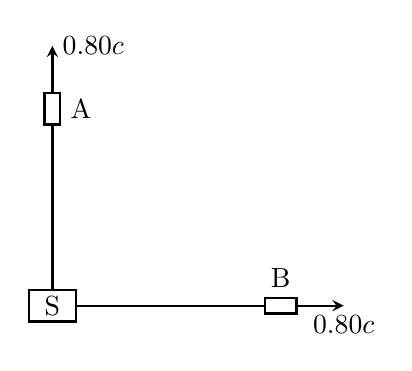
\begin{tikzpicture}[>=stealth, thick]
    % S station
    \draw (0,0) rectangle (0.6, 0.4);
    \node at (0.3, 0.2) {S};
    
    % Track for B
    \draw (0.6, 0.2) -- (3, 0.2);
    % Train B
    \draw[fill=white] (3, 0.1) rectangle (3.4, 0.3);
    \node[above] at (3.2, 0.3) {B};
    \draw[->] (3.4, 0.2) -- (4, 0.2) node[below] {$0.80c$};
    
    % Track for A
    \draw (0.3, 0.4) -- (0.3, 2.5);
    % Train A
    \draw[fill=white] (0.2, 2.5) rectangle (0.4, 2.9);
    \node[right] at (0.4, 2.7) {A};
    \draw[->] (0.3, 2.9) -- (0.3, 3.5) node[right] {$0.80c$};
\end{tikzpicture}
\end{center}
\end{exercise}
\begin{solution}

\end{solution}

\begin{exercise}\label{ex:9.14}
太阳流向地球的能流是 $1340 \ \mathrm{W/m^2}$. 问每年太阳有多少质量流向地球？
\end{exercise}
\begin{solution}

\end{solution}

\begin{exercise}\label{ex:9.15}
$20\mathrm{-kt}$ 核弹需要多少裂变物质？(对于 TNT，燃烧值为 $C = 4.18 \times 10^9 \ \mathrm{J/t}$)
\end{exercise}
\begin{solution}

\end{solution}

\begin{exercise}\label{ex:9.16}
自由中子衰变过程为
$$ \mathrm{n} \longrightarrow \mathrm{p} + \mathrm{e}^- + \nu $$
设自由中子原来静止，衰变后的质子也静止，求电子的动能.
\end{exercise}
\begin{solution}

\end{solution}

\begin{exercise}\label{ex:9.17}
一个动能为 $250 \ \mathrm{MeV}$ 的 $\Sigma^-$ 衰变如下：
$$ \Sigma^- \longrightarrow \pi^- + \mathrm{n} $$
$\pi$ 介子与 $\Sigma^-$ 原来的运动方向成 $90^\circ$ 夹角. 求 $\pi$ 介子和中子的动能以及中子的运动方向.
\end{exercise}
\begin{solution}

\end{solution}

\begin{exercise}\label{ex:9.18}
高能加速器将质量为 $m$ 的粒子束加速到总能 $E_b$，然后用之去轰击静止靶，但是用较低的能量 $E'$ 的两束粒子能导致同样的碰撞，如图所示. 证明
\begin{enumerate}
  \item[(a)] $$ \beta_{\mathrm{com}} = \frac{E_b - mc^2}{p_bc} = \frac{p_bc}{E_b + mc^2} $$
  \item[(b)] $$ E' = \left[ \frac{1}{2}mc^2(E_b + mc^2) \right]^{1/2} $$
\end{enumerate}
\begin{center}
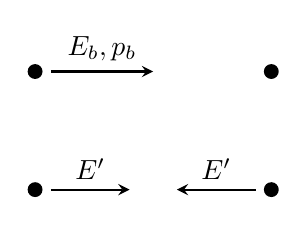
\begin{tikzpicture}[>=stealth, thick]
    % Top part (Fixed target)
    \filldraw[black] (0, 1.5) circle (0.08);
    \draw[->] (0.2, 1.5) -- (1.5, 1.5);
    \node[above] at (0.85, 1.5) {$E_b, p_b$};
    \filldraw[black] (3, 1.5) circle (0.08);
    
    % Bottom part (Colliding beams)
    \filldraw[black] (0, 0) circle (0.08);
    \draw[->] (0.2, 0) -- (1.2, 0);
    \node[above] at (0.7, 0) {$E'$};
    
    \filldraw[black] (3, 0) circle (0.08);
    \draw[->] (2.8, 0) -- (1.8, 0);
    \node[above] at (2.3, 0) {$E'$};
\end{tikzpicture}
\end{center}
\end{exercise}
\begin{solution}

\end{solution}

\begin{exercise}\label{ex:9.19}
对 $\gamma \gg 1$，证明下式成立：
$$ p \approx \left(1 - \frac{1}{2\gamma^2}\right)\frac{E}{c} $$
\end{exercise}
\begin{solution}

\end{solution}

\begin{exercise}\label{ex:9.20}
$\mu$ 子静止质量为 $m_0 = 105 \ \mathrm{MeV/c^2}$，半衰期为 $\tau = 2 \times 10^{-6} \ \mathrm{s}$. 在 $t=0$ 时一 $\mu$ 子从加速器中产生，此时动能为 $10395 \ \mathrm{MeV}$.
\begin{enumerate}
  \item[(a)] $\mu$ 子的总能量是多少？
  \item[(b)] $\gamma$ 值是什么？
  \item[(c)] 速度和动量是多少？
  \item[(d)] 在实验室系中半衰期是多少？
  \item[(e)] 衰变掉以前，它能飞多远？
\end{enumerate}
\end{exercise}
\begin{solution}

\end{solution}
\chapter{第十章 温度}

1. (a) $-40$; (b) $575$; (c) N.A.

5. $0.27\text{mm}$

7. $B(T) = b - \frac{a}{RT^2}$

\begin{exercise}\label{ex:10.1}
在下列成对的温标中，什么温度有相同的读数？
\begin{enumerate}
  \item[(a)] 华氏和摄氏；
  \item[(b)] 华氏和开氏；
  \item[(c)] 摄氏和开氏.
\end{enumerate}
\end{exercise}
\begin{solution}

\end{solution}

\begin{exercise}\label{ex:10.2}
考虑一个水银温度计. 设其毛细管的横截面积为常量 $A_0$，$0.00^\circ\mathrm{C}$ 时水银泡的体积为 $V_0$. 若水银恰是在 $0.00^\circ\mathrm{C}$ 时灌入的，试证明在 $t^\circ\mathrm{C}$ 时水银柱的长度可以表示为
$$l = \frac{V_0}{A_0}(\beta - 3\alpha)t$$
即其长度正比于温度；式中 $\beta$ 是水银的体膨胀系数，$\alpha$ 是玻璃的线膨胀系数.
\end{exercise}
\begin{solution}

\end{solution}

\begin{exercise}\label{ex:10.3}
\begin{enumerate}
  \item[(a)] 证明固体的转动惯量 $I$ 随温度 $T$ 的改变可表示为 $\Delta I = 2\alpha I \Delta T$；
  \item[(b)] 证明物理摆的周期 $t$ 随温度的变化为 $\Delta t = \alpha t \Delta T / 2$.
\end{enumerate}
\end{exercise}
\begin{solution}

\end{solution}

\begin{exercise}\label{ex:10.4}
如图，铝质圆柱用柔软的钢条对称地悬挂于两面直立的墙之间，要求圆柱的轴线 $C$ 不因圆柱或钢条的热胀冷缩而有所改变，当 $T = 290 \ \mathrm{K}$，$L = 2.5 \ \mathrm{m}$，$\theta = 50^\circ$ 时求圆柱的半径 $R$. 如果取近似，应讨论其合理性. (忽略钢条的重量；钢的线膨胀系数为 $1.1 \times 10^{-5} \ \mathrm{K}^{-1}$，而铝的线膨胀系数为 $2.3 \times 10^{-5} \ \mathrm{K}^{-1}$)
\begin{center}
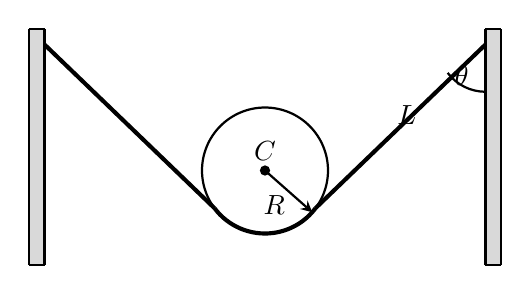
\begin{tikzpicture}[>=stealth, thick]
    % Walls
    \fill[gray!30] (-3, 0) rectangle (-2.8, 3);
    \draw (-2.8, 0) -- (-2.8, 3);
    \draw (-3, 0) -- (-3, 3);
    \draw (-3, 0) -- (-2.8, 0);
    \draw (-3, 3) -- (-2.8, 3);

    \fill[gray!30] (2.8, 0) rectangle (3, 3);
    \draw (2.8, 0) -- (2.8, 3);
    \draw (3, 0) -- (3, 3);
    \draw (3, 0) -- (2.8, 0);
    \draw (3, 3) -- (2.8, 3);

    % Cylinder
    \draw (0, 1.2) circle (0.8);
    \filldraw[black] (0, 1.2) circle (0.05);
    \node[above] at (0, 1.2) {$C$};
    
    % Radius R
    \draw[->] (0, 1.2) -- (0.6, 0.67) node[midway, below left, inner sep=1pt] {$R$};

    % Steel Strip
    \draw[line width=1.5pt] (-2.8, 2.8) -- (-0.64, 0.72);
    \draw[line width=1.5pt] (2.8, 2.8) -- (0.64, 0.72);
    \draw[line width=1.5pt] (-0.64, 0.72) arc (216.87:323.13:0.8);

    % Labels
    \node at (1.8, 1.9) {$L$};
    \draw (2.8, 2.2) arc (270:216.87:0.6);
    \node at (2.5, 2.4) {$\theta$};
\end{tikzpicture}
\end{center}
\end{exercise}
\begin{solution}

\end{solution}

\begin{exercise}\label{ex:10.5}
边长为 $20 \ \mathrm{cm}$ 的立方块飘浮在水银面上. 若温度从 $270 \ \mathrm{K}$ 上升至 $320 \ \mathrm{K}$，计算铝块浸入水银的深度的改变. (水银的膨胀系数为 $1.8 \times 10^{-4} \ \mathrm{K}^{-1}$)
\end{exercise}
\begin{solution}

\end{solution}

\begin{exercise}\label{ex:10.6}
所谓 6-12 势如(5.3.1)式所示：
$$U = 4\varepsilon \left[ \left(\frac{\sigma}{r}\right)^{12} - \left(\frac{\sigma}{r}\right)^6 \right]$$
\begin{enumerate}
  \item[(a)] 求势能曲线的极值位置和极值大小. 
  \item[(b)] 求当总能量为极值的 $0.8$ 时，分子的运动范围和平均距离. 
  \item[(c)] 相对膨胀率是多少？
  \item[(d)] 作势能曲线示意图，标明 $\sigma$ 以及(a)、(b)中的结果.
\end{enumerate}
\end{exercise}
\begin{solution}

\end{solution}

\begin{exercise}\label{ex:10.7}
Berthelot 状态方程为
$$\left( p + \frac{an^2}{TV^2} \right)(V - nb) = nRT$$
求它的第二位力系数.
\end{exercise}
\begin{solution}

\end{solution}
\chapter{第十一章 热力学第一定律}

1. (a) 没有, (b) 有, (c) 有, $93\text{J/kg}$
(d) $0.19\text{K}$

3. (a) $n = n_0 \exp(-mgh/k_B T)$
(b) $\frac{\text{d}T}{\text{d}z} = - \frac{\gamma - 1}{\gamma} \frac{mg}{k_B T}$

5. $\frac{1}{2\pi} \sqrt{\frac{\gamma A^2 \left(p_0 + \frac{mg}{A}\right)}{V_0 m}}$

7. $RT = \text{const.}$

9. $\eta = 1 - \left(\frac{p_A}{p_B}\right)^{\frac{\gamma - 1}{\gamma}}$

13. $p_0 V_0 \left( \frac{2^{\gamma - 1} - 1}{\gamma - 1} - \ln 2 \right)$

15. 白天 $10.9\text{kW}$, 夜晚 $24.6\text{kW}$

\begin{exercise}\label{ex:11.1}
一铁球从 $10 \ \mathrm{m}$ 高处落至水泥地面上，第一次回跳高度为 $0.50 \ \mathrm{m}$. 假设碰撞过程中机械能的损失只导致铁球能量的变化. 
\begin{enumerate}
  \item[(a)] 有没有热加到铁球上？
  \item[(b)] 有没有对铁球做功？
  \item[(c)] 铁球的内能有没有变化？如果有，数值是多大？
  \item[(d)] 铁的比热容是 $0.50 \ \mathrm{kJ/(kg \cdot K)}$，铁球温度升高多少？
\end{enumerate}
\end{exercise}
\begin{solution}

\end{solution}

\begin{exercise}\label{ex:11.2}
一种物质具有如下状态方程：
$$p = AT^3/V$$
其中 $p$、$V$ 及 $T$ 分别为压强、体积和温度，$A$ 为一个常量. 该物质的内能为
$$U = BT^n \ln(V/V_0) + f(T)$$
其中 $B$、$n$ 及 $V_0$ 均为常量，$f(T)$ 只依赖于温度. 试确定 $B$ 及 $n$.
\end{exercise}
\begin{solution}

\end{solution}

\begin{exercise}\label{ex:11.3}
考虑大气的一个简单模型，不计风、对流及重力随高度变化等的因素.
\begin{enumerate}
  \item[(a)] 设大气是等温的，求分子密度随高度的分布；
  \item[(b)] 假设大气是绝热的，证明此时温度随高度的增加而线性减小，并求减小的速率.
\end{enumerate}
\end{exercise}
\begin{solution}

\end{solution}

\begin{exercise}\label{ex:11.4}
一定质量的气体在 $101325 \ \mathrm{Pa}$ 和 $300 \ \mathrm{K}$ 时占据 $4.0 \times 10^{-3} \ \mathrm{m^3}$ 的体积，现将其绝热压缩至 $1.0 \times 10^{-3} \ \mathrm{m^3}$，确定
\begin{enumerate}
  \item[(a)] 压缩后的压强、
  \item[(b)] 气体最后的温度.
\end{enumerate}
设该气体为理想气体，且比热比为 $\gamma = 1.5$.
\end{exercise}
\begin{solution}

\end{solution}

\begin{exercise}\label{ex:11.5}
一容器体积为 $V_0$(如图)，装有理想气体. 玻璃管的横截面积为 $A$，有一个质量为 $m$ 的小球正好封住管子并可以在管内无摩擦滑动. 大气压为 $p_0$，管内压力略高于大气压. 如果小球略偏离平衡位置，它将作简谐振动. 设气体经历的过程是绝热的，$\gamma$ 是比热比，求小球振动频率.
\begin{center}
\begin{tikzpicture}[>=stealth, thick]
    % Container body
    \draw (-1.5, -2.5) -- (-1.5, 0) -- (-0.4, 0);
    \draw (1.5, -2.5) -- (1.5, 0) -- (0.4, 0);
    \draw (-1.5, -2.5) -- (1.5, -2.5);
    \node at (0, -1.2) {$V_0$};
    
    % Glass tube
    \draw (-0.4, 0) -- (-0.4, 1.2);
    \draw (0.4, 0) -- (0.4, 1.2);
    
    % Shaded support/flange area
    \fill[pattern=north east lines, pattern color=gray!80] (-0.8, 0.3) rectangle (-0.4, 0.9);
    \fill[pattern=north east lines, pattern color=gray!80] (0.4, 0.3) rectangle (0.8, 0.9);
    \draw (-0.8, 0.3) -- (-0.8, 0.9) -- (-0.4, 0.9) -- (-0.4, 0.3) -- cycle;
    \draw (0.4, 0.3) -- (0.8, 0.3) -- (0.8, 0.9) -- (0.4, 0.9) -- cycle;
    
    % Ball
    \shade[ball color=black!80] (0, 0.9) circle (0.25);
    \node[right] at (0.3, 0.9) {$m$};
\end{tikzpicture}
\end{center}
\end{exercise}
\begin{solution}

\end{solution}

\begin{exercise}\label{ex:11.6}
小振幅纵波在理想气体中的速度为
$$ c = \sqrt{\frac{\mathrm{d}p}{\mathrm{d}\rho}} $$
式中 $p$ 为作为介质的气体的压强，$\rho$ 为相应气体的密度，试推导：
\begin{enumerate}
  \item[(a)] 等温压缩或等温膨胀时气体中的声速；
  \item[(b)] 绝热压缩或绝热膨胀时气体中的声速.
\end{enumerate}
\end{exercise}
\begin{solution}

\end{solution}

\begin{exercise}\label{ex:11.7}
在宇宙大爆炸理论中，起初局限于小区域的辐射能量以球对称方式绝热膨胀，在膨胀的过程中辐射逐渐冷却. 仅仅从热力学的角度考虑，试推导出温度 $T$ 和辐射半径 $R$ 的关系.
\end{exercise}
\begin{solution}

\end{solution}

\begin{exercise}\label{ex:11.8}
一可逆热机以 $1.00 \ \mathrm{mol}$ 单原子理想气体作工作物质并经历图示的循环过程. 其中状态 2 至状态 3 为绝热过程.
\begin{enumerate}
  \item[(a)] 分别对三个不同过程及整个循环计算热量的变化、内能的改变及气体所作的功；
  \item[(b)] 若在状态 1 的初始压强为 $101325 \ \mathrm{Pa}$，计算气体在状态 2 和状态 3 时的体积及压强.
\end{enumerate}
\begin{center}
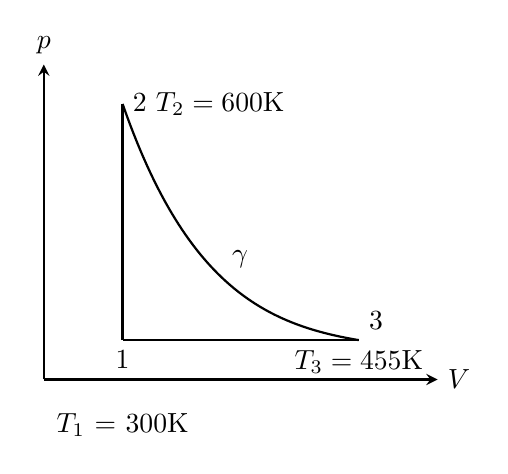
\begin{tikzpicture}[>=stealth, thick]
    % Axes
    \draw[->] (0, 0) -- (5, 0) node[right] {$V$};
    \draw[->] (0, 0) -- (0, 4) node[above] {$p$};
    
    % Points
    \coordinate (P1) at (1, 0.5);
    \coordinate (P2) at (1, 3.5);
    \coordinate (P3) at (4, 0.5);
    
    % Lines
    \draw (P1) -- (P2);
    \draw (P2) .. controls (1.8, 1.2) and (2.8, 0.7) .. (P3) node[midway, right=4pt, above=2pt] {$\gamma$};
    \draw (P3) -- (P1);
    
    % Labels
    \node[below] at (P1) {$1$};
    \node[below, text width=2cm, align=center] at (1, -0.3) {$T_1=300\mathrm{K}$};
    \node[right] at (P2) {$2 \ T_2=600\mathrm{K}$};
    \node[above right] at (P3) {$3$};
    \node[below] at (P3) {$T_3=455\mathrm{K}$};
\end{tikzpicture}
\end{center}
\end{exercise}
\begin{solution}

\end{solution}

\begin{exercise}\label{ex:11.9}
理想的气涡轮机作 Joule 循环(如图)，所有过程都是准静的. 其中 $A$ 到 $B$ 和 $C$ 到 $D$ 为绝热过程. 设热机中的工作物质为理想气体，其定压与定体比热之比为 $\gamma$. 求热机的效率，用压强比来表示.
\begin{center}
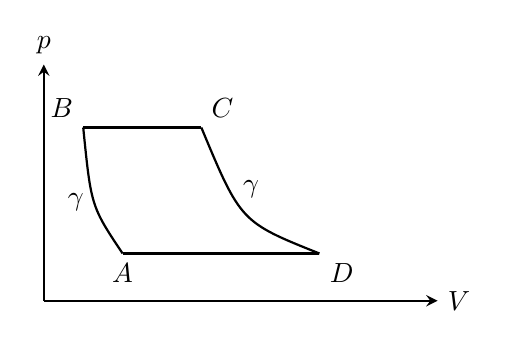
\begin{tikzpicture}[>=stealth, thick]
    % Axes
    \draw[->] (0, 0) -- (5, 0) node[right] {$V$};
    \draw[->] (0, 0) -- (0, 3) node[above] {$p$};
    
    % Points
    \coordinate (A) at (1, 0.6);
    \coordinate (B) at (0.5, 2.2);
    \coordinate (C) at (2, 2.2);
    \coordinate (D) at (3.5, 0.6);
    
    % Lines
    \draw (A) .. controls (0.6, 1.2) .. (B) node[midway, left] {$\gamma$};
    \draw (B) -- (C);
    \draw (C) .. controls (2.5, 1.0) .. (D) node[midway, right=2pt, above=2pt] {$\gamma$};
    \draw (D) -- (A);
    
    % Labels
    \node[below] at (A) {$A$};
    \node[above left] at (B) {$B$};
    \node[above right] at (C) {$C$};
    \node[below right] at (D) {$D$};
\end{tikzpicture}
\end{center}
\end{exercise}
\begin{solution}

\end{solution}

\begin{exercise}\label{ex:11.10}
一可逆热机以 $1 \ \mathrm{mol}$ 双原子理想气体作工作物质按图作 Otto 循环过程. 试以图中所标出的体积表示热机的效率.
\begin{center}
\begin{tikzpicture}[>=stealth, thick]
    % Axes
    \draw[->] (0, 0) -- (5, 0) node[right] {$V$};
    \draw[->] (0, 0) -- (0, 4) node[above] {$p$};
    
    % Points
    \coordinate (P1) at (1.2, 3.8);
    \coordinate (P4) at (1.2, 2.0);
    \coordinate (P2) at (4, 1.0);
    \coordinate (P3) at (4, 0.4);
    
    % Solid Lines
    \draw (P1) .. controls (1.8, 1.5) and (3, 1.2) .. (P2) node[midway, right=2pt, above=2pt] {$\gamma$};
    \draw (P2) -- (P3);
    \draw (P4) .. controls (1.8, 0.8) and (3, 0.5) .. (P3) node[midway, right=2pt, above=2pt] {$\gamma$};
    \draw (P4) -- (P1);
    
    % Dashed Lines
    \draw[dashed] (P4) -- (1.2, 0) node[below] {$V_1$};
    \draw[dashed] (P3) -- (4, 0) node[below] {$V_2$};
    
    % Labels
    \node[left] at (P1) {$1$};
    \node[left] at (P4) {$4$};
    \node[right] at (P2) {$2$};
    \node[right] at (P3) {$3$};
    \node at (3.5, 3.2) {Otto 循环};
\end{tikzpicture}
\end{center}
\end{exercise}
\begin{solution}

\end{solution}

\begin{exercise}\label{ex:11.11}
若卡诺热机逆向运转，我们将得到一理想的制冷机. 热量 $Q_2$ 由温度为 $T_2$ 的低温热源获得，然后向温度为 $T_1$ 的高温热源传送热量 $Q_1$，同时外界需对热机做功 $W$ 以使之运行.
\begin{enumerate}
  \item[(a)] 证明
  $$ W = Q_2 \frac{T_1 - T_2}{T_2} $$
  \item[(b)] 制冷机的操作系数 $K$ 一般定义为从低温热源吸收的热量与外界对之所做的功之比，即 $K = Q_2/W$，证明在理想状态下 $K$ 可表示为
  $$ K = \frac{T_2}{T_1 - T_2} $$
\end{enumerate}
实际情况中 $K$ 一般为 5 或 6.
\end{exercise}
\begin{solution}

\end{solution}

\begin{exercise}\label{ex:11.12}
一个空调装置可以用来降低室内温度，它实质上是一个制冷器，通过外界做功把热量从室内(温度较低)抽取出来释放到室外(温度较高). 设室内的温度为 $T_2$，室外的温度为 $T_1 > T_2$，空调设备按可逆卡诺循环运行，其消耗功率为 $P$.
\begin{enumerate}
  \item[(a)] 每秒钟空调设备从室内抽取 $Q_2$ 的热量并向室外放出 $Q_1$ 的热量. 试用 $T_1$ 和 $T_2$ 来表示空调设备的工作效率 $Q_2/P$.
  \item[(b)] 如果空调设备只工作 $30\%$ 的时间就可以在室外温度为 $30^\circ\mathrm{C}$ 时使室内温度保持在 $20^\circ\mathrm{C}$. 试问用此设备使室内温度保持在 $20^\circ\mathrm{C}$ 时，室外温度最高可达多少？
\end{enumerate}
\end{exercise}
\begin{solution}

\end{solution}

\begin{exercise}\label{ex:11.13}
具有系数 $\gamma$ 的气体最初在汽缸中的体积为 $V_0$，压强为 $p_0$，然后缓慢地、绝热地压缩到 $V_0/2$. 在该体积下，让气体达到平衡温度后，又让它缓慢并且等温地膨胀到原始体积 $V_0$. 试求活塞对气体所作的净功，用 $p_0$、$V_0$ 来表示.
\end{exercise}
\begin{solution}

\end{solution}

\begin{exercise}\label{ex:11.14}
一个为压缩氮气而设计的压缩机用来压缩空气时出现了过热现象，假定压缩机是近似绝热的，并且此两气体的初始压强相同，试解释这种现象.
\end{exercise}
\begin{solution}

\end{solution}

\begin{exercise}\label{ex:11.15}
地球上的人要在月球上居住，首要问题就是保持他们的起居室处于一个舒适的温度. 现考虑用卡诺热机来作温度调节. 设月球的昼间温度为 $100^\circ\mathrm{C}$，而夜间温度为 $-100^\circ\mathrm{C}$，起居室温度要保持在 $20^\circ\mathrm{C}$. 通过起居室墙壁导热的速率为每度温差 $0.5 \ \mathrm{kW}$，试求昼间与夜间所需供给卡诺热机的功率.
\end{exercise}
\begin{solution}

\end{solution}
\chapter{第十二章 热力学第二定律}

1. (a) $1.30\text{kJ/K}, -1.12\text{kJ/K}, 0.18\text{kJ/K}$,
(b) $0.096\text{kJ/K}$

3. 当 $N \to \infty, \Delta S = 0$

5. $562.77\text{K}$

7. (a) $\sqrt{c(T_1 + T_2 - 2T)}$
(b) $\sqrt{c(T_1 + T_2 - 2\sqrt{T_1 T_2})}$

9. [图片：循环过程曲线图]

\begin{exercise}\label{ex:12.1}
水的比热容为 $4.186 \ \mathrm{kJ/(kg \cdot K)}$，可近似看成与温度无关.
\begin{enumerate}
  \item[(a)] $0^\circ\mathrm{C}$ 的 $1.0 \ \mathrm{kg}$ 水突然与 $100^\circ\mathrm{C}$ 的热库接触，当水达到 $100^\circ\mathrm{C}$ 时，求水和热库的总熵变.
  \item[(b)] 如果 $0^\circ\mathrm{C}$ 的 $1.0 \ \mathrm{kg}$ 水先与 $50^\circ\mathrm{C}$ 的热库接触，平衡后再与 $100^\circ\mathrm{C}$ 的热库接触，求整个系统的熵变.
\end{enumerate}
\end{exercise}
\begin{solution}

\end{solution}

\begin{exercise}\label{ex:12.2}
假设某系统的熵 $S$、体积 $V$、内能 $U$ 和粒子数 $N$ 之间的关系为
$$ S = A(nVU)^{1/3} $$
其中 $A$ 为常量. 求下列各物理量之间的关系：
\begin{enumerate}
  \item[(a)] $U$、$n$、$V$ 和 $T$；
  \item[(b)] $p$、$n$、$V$ 和 $T$，以及
  \item[(c)] 系统的定容比热.
\end{enumerate}
\end{exercise}
\begin{solution}

\end{solution}

\begin{exercise}\label{ex:12.3}
温度为 $T_{\mathrm{i}}$ 的一物质依次与温度为 $T_{\mathrm{i}} + \Delta T, T_{\mathrm{i}} + 2\Delta T, \dots, T_{\mathrm{i}} + N\Delta T = T_{\mathrm{f}}$ 的热源相接触而使自身温度变为 $T_{\mathrm{f}}$. 假定物质的热容与温度 $T$ 无关，计算由物质和热源构成的整个系统的总熵变. 在 $N \to \infty$ 而 $T_{\mathrm{f}} - T_{\mathrm{i}}$ 不变时，其熵变是多少？
\end{exercise}
\begin{solution}

\end{solution}

\begin{exercise}\label{ex:12.4}
两个全同的物体，其内能为 $U = CT$，式中 $C$ 为常量. 初始时两物体的温度分别为 $T_1$ 和 $T_2$. 现在分别以两物体作为高低温热源驱动一卡诺热机运行，最后两物体达到一共同温度 $T_{\mathrm{f}}$. 求：
\begin{enumerate}
  \item[(a)] $T_{\mathrm{f}}$；
  \item[(b)] 卡诺热机所做的功.
\end{enumerate}
\end{exercise}
\begin{solution}

\end{solution}

\begin{exercise}\label{ex:12.5}
3 个有限大物体热容为常量，开始时分别处于 $400 \ \mathrm{K}$、$400 \ \mathrm{K}$ 和 $100 \ \mathrm{K}$ 的温度下. 如果用热机或制冷机工作其间以提高其中一个物体的温度，问最高可能温度是多少？
\end{exercise}
\begin{solution}

\end{solution}

\begin{exercise}\label{ex:12.6}
现在有两个完全一样的物体，其热力学性质由 12.2 题中的状态方程所描述. 初始温度分别是 $T_1$ 和 $T_2$，有一热机工作于这两个物体之间，最终两物体达到一共同温度 $T_{\mathrm{f}}$. 
\begin{enumerate}
  \item[(a)] 求温度 $T_{\mathrm{f}}$ 的范围；
  \item[(b)] 求最大功 $W_{\max}$.
\end{enumerate}
求解这些问题时，可以考虑可逆过程，也可以考虑不可逆过程.
\end{exercise}
\begin{solution}

\end{solution}

\begin{exercise}\label{ex:12.7}
考虑如图所示的水力机. 从左端输入温度分别为 $T_1$ 和 $T_2$ 的等量的冷热水稳流，从右端输出唯一的水的喷流. 假设单位质量水的热容 $c$ 与温度无关. 机器处于稳定的工作状态，其输入水流的动能可以忽略不计. 
\begin{enumerate}
  \item[(a)] 用 $T_1$、$T_2$ 和 $T$ 表示喷出水的速率，其中 $T$ 为喷口处水的温度.
  \item[(b)] 最大可能的喷出速率是多少？
\end{enumerate}
\begin{center}
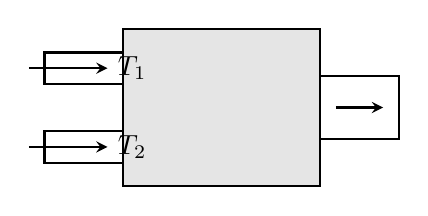
\begin{tikzpicture}[>=stealth, thick]
    % Machine Body
    \draw[fill=gray!20] (0, 0) rectangle (2.5, 2);
    
    % Top Input (T1)
    \draw[fill=white] (-1, 1.3) rectangle (0, 1.7);
    \draw[->] (-1.2, 1.5) -- (-0.2, 1.5) node[right] {$T_1$};
    
    % Bottom Input (T2)
    \draw[fill=white] (-1, 0.3) rectangle (0, 0.7);
    \draw[->] (-1.2, 0.5) -- (-0.2, 0.5) node[right] {$T_2$};
    
    % Output
    \draw[fill=white] (2.5, 0.6) rectangle (3.5, 1.4);
    \draw[->] (2.7, 1.0) -- (3.3, 1.0);
\end{tikzpicture}
\end{center}
\end{exercise}
\begin{solution}

\end{solution}

\begin{exercise}\label{ex:12.8}
一温度为 $60^\circ\mathrm{C}$ 的子弹以 $400 \ \mathrm{m/s}$ 速度撞击并嵌入一大的障碍物. 障碍物温度为 $15^\circ\mathrm{C}$. 子弹的质量为 $20 \times 10^{-3} \ \mathrm{kg}$、比热为 $400 \ \mathrm{J/(kg \cdot K)}$. 求过程中总的熵变.
\end{exercise}
\begin{solution}

\end{solution}

\begin{exercise}\label{ex:12.9}
W. Atkins 设计的棋盘游戏：棋盘为 $40 \times 40$ 格，中间 $10 \times 10 = 100$ 格为系统 I，外部 1500 格点为系统 II (如图). 开始时 100 个棋子全部集中在系统 I. 此时两个子系统的熵均为零，整个棋盘系统的熵也为零. 当有一个棋子从系统 I 移到系统 II 时，系统的熵分别为
\begin{align*}
  S_{\mathrm{I}} &= k_{\mathrm{B}} \ln 100 = 4.61 k_{\mathrm{B}} \\
  S_{\mathrm{II}} &= k_{\mathrm{B}} \ln 1500 = 7.31 k_{\mathrm{B}} \\
  S &= S_{\mathrm{I}} + S_{\mathrm{II}} = 11.92 k_{\mathrm{B}}
\end{align*}
\begin{enumerate}
  \item[(a)] 以系统 II 中的棋子数为横轴，作三条熵曲线.
  \item[(b)] 求系统熵的极值.
  \item[(c)] 求系统熵处于极值时，子系统 I 和 II 中的密度.
\end{enumerate}
\begin{center}
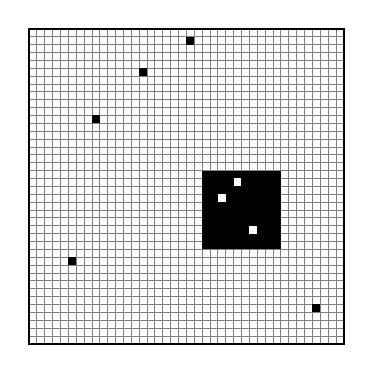
\begin{tikzpicture}[>=stealth, thick]
    % Simulated 40x40 grid using 4x4 with 0.1 steps
    \draw[step=0.1, gray, very thin] (0,0) grid (4,4);
    \draw (0,0) rectangle (4,4);
    
    % System I (10x10 area = 1x1 in current coordinates)
    \fill[black] (2.2, 1.2) rectangle (3.2, 2.2);
    
    % White pieces in System I
    \fill[white] (2.4, 1.8) rectangle (2.5, 1.9);
    \fill[white] (2.8, 1.4) rectangle (2.9, 1.5);
    \fill[white] (2.6, 2.0) rectangle (2.7, 2.1);
    
    % Black pieces in System II
    \fill[black] (0.8, 2.8) rectangle (0.9, 2.9);
    \fill[black] (1.4, 3.4) rectangle (1.5, 3.5);
    \fill[black] (3.6, 0.4) rectangle (3.7, 0.5);
    \fill[black] (0.5, 1.0) rectangle (0.6, 1.1);
    \fill[black] (2.0, 3.8) rectangle (2.1, 3.9);
\end{tikzpicture}
\end{center}
\end{exercise}
\begin{solution}

\end{solution}

\begin{exercise}\label{ex:12.10}
橡皮带绝热拉伸时变热. 当加热而保持张力不变时，橡皮带将膨胀还是收缩？
\end{exercise}
\begin{solution}

\end{solution}

\begin{exercise}\label{ex:12.11}
证明：
$$ \left(\frac{\partial C_V}{\partial V}\right)_T = T \left(\frac{\partial^2 p}{\partial T^2}\right)_V, \quad \left(\frac{\partial C_p}{\partial p}\right)_T = -T \left(\frac{\partial^2 V}{\partial T^2}\right)_p $$
\end{exercise}
\begin{solution}

\end{solution}

\begin{exercise}\label{ex:12.12}
证明：
$$ \left(\frac{\partial \mu}{\partial V_m}\right)_T = V_m \left(\frac{\partial p}{\partial V_m}\right)_T $$
\end{exercise}
\begin{solution}

\end{solution}

\begin{exercise}\label{ex:12.13}
证明：
$$ T \mathrm{d}S = C_p \mathrm{d}T - TV\alpha \mathrm{d}p, \quad T \mathrm{d}S = C_V \mathrm{d}T + T \frac{\alpha}{\kappa} \mathrm{d}V $$
式中 $\alpha$ 和 $\kappa$ 分别为膨胀系数和等温压缩率.
\end{exercise}
\begin{solution}

\end{solution}

\begin{exercise}\label{ex:12.14}
证明：
$$ \frac{\kappa_T}{\kappa_S} = \frac{C_p}{C_V} $$
从而说明等温压缩率大于绝热压缩率.
\end{exercise}
\begin{solution}

\end{solution}
\chapter{第十三章 理想气体的微观模型}

1. $v \approx c$

3. $p_1(t) = \frac{p_0}{2} \left[ 1 + \text{e}^{-\frac{Avt}{2V}} \right]$

5. (1) $v_s = 350\text{m/s}$
(2) $f = 1.2 \times 10^8\text{Hz}$
(3) $\bar{\ell} = 4 \times 10^{-6}\text{m}$
(4) $\bar{\ell}/\lambda = 3.4 \times 10^{-6}$

9. $W = n \left( \frac{k_B T}{2\pi m} \right)^{\frac{1}{2}} \text{e}^{-\frac{mv_e^2}{2k_B T}}$

11. $51\text{K}$

13. (a) $T_{\oplus} = 17^\circ\text{C}$
(b) $6 \times 10^8\text{N}$

\begin{exercise}\label{ex:13.1}
质量为 $1000 \ \mathrm{kg}$ 的火箭射入太空. 假设所有星体具有相同的平均质量 $10^{33} \ \mathrm{kg}$，并以平均速率 $10 \ \mathrm{km/s}$ 作随机运动. 那么，该火箭发射了相当长时间后，平均速率 $v$ 为多少？
\end{exercise}
\begin{solution}

\end{solution}

\begin{exercise}\label{ex:13.2}
$^{23}\mathrm{Na}$ 蒸气在气体放电管中发射 $598 \ \mathrm{nm}$ 的强黄线. 如果蒸气处于室温，试粗略估计由于热运动而引起的多普勒频移使这条谱线显示的宽度是多少 $\mathrm{nm}$.
\end{exercise}
\begin{solution}

\end{solution}

\begin{exercise}\label{ex:13.3}
一体积为 $2V$ 的盒子被一薄片分为体积相等的两部分. 初始时，左边含有压强为 $p_0$ 的理想气体，右边为真空；隔片上开有面积为 $A$ 的小孔. 试求左边压强 $p_1$ 随时间变化的函数关系. 假定两边温度都是常量，将结果用平均速度 $v$ 表示出来.
\end{exercise}
\begin{solution}

\end{solution}

\begin{exercise}\label{ex:13.4}
体积相等($V_1 = V_2 = V$)的两个容器，用小“针孔”管连接起来. 这两个容器分别保持在恒温 $T_1$ 和 $T_2$ 下. 所有的气体分子都具有质量 $m$. 压强比仅为 $T_1$ 和 $T_2$ 的函数. 求压强比.
\end{exercise}
\begin{solution}

\end{solution}

\begin{exercise}\label{ex:13.5}
稀薄气体中的声速 $v_s$，由绝热压缩率表示：
$$ v_s = \left[ \left( \frac{\partial \rho}{\partial p} \right)_S \right]^{-1/2} $$
\begin{enumerate}
  \item[(a)] 对室温下的空气，求下列数值结果：(1)声速；(2)平均分子碰撞频率；(3)分子平均自由程；(4)平均自由程与声波波长之比.
  \item[(b)] 用上述结果解释为什么绝热近似是合理的假设.
\end{enumerate}
采用 $m$ 为分子的平均质量，$k_{\mathrm{B}}$ 为玻耳兹曼常量，$\gamma$ 为热容比.
\end{exercise}
\begin{solution}

\end{solution}

\begin{exercise}\label{ex:13.6}
求速率大于最概然速率的分子数.
\end{exercise}
\begin{solution}

\end{solution}

\begin{exercise}\label{ex:13.7}
推导二维平衡速率分布.
\end{exercise}
\begin{solution}

\end{solution}

\begin{exercise}\label{ex:13.8}
推导平衡能量分布.
\end{exercise}
\begin{solution}

\end{solution}

\begin{exercise}\label{ex:13.9}
温度为 $T$、分子质量为 $m$ 的气体满足麦克斯韦速度分布. 一个干净的固体表面暴露在此气体中时，它以速率 $W(\mathrm{s^{-1}\cdot cm^{-2}})$ 吸收分子. 如果某一分子的法向速度分量小于 $v_T$ 时吸收概率为 $0$，大于 $v_T$ 时的吸收概率为 $1$. 试推导 $W$ 的表达式. (分子数密度为 $n$)
\end{exercise}
\begin{solution}

\end{solution}

\begin{exercise}\label{ex:13.10}
气体分子从容器壁上的小孔中泻出，求其能量的平均值. 设温度为 $T$，气体分子数密度为 $n$.
\end{exercise}
\begin{solution}

\end{solution}

\begin{exercise}\label{ex:13.11}
已知：平均日-地距离为 $1.5 \times 10^8 \ \mathrm{km}$；平均日-海王星距离为 $4.5 \times 10^9 \ \mathrm{km}$. 试作出合理的假设，以估计海王星的表面温度. 忽略任何可能的内部热源.
\end{exercise}
\begin{solution}

\end{solution}

\begin{exercise}\label{ex:13.12}
太阳的辐射近似于一个温度为 $5700 \ \mathrm{K}$ 的黑体. 若有一个理想的黑色铜球在离太阳 $1 \ \mathrm{AU}$ 的距离处受到日光的辐射，它将达到多高的平衡温度？(太阳直径对地球张角为 $0.50^\circ$)
\end{exercise}
\begin{solution}

\end{solution}

\begin{exercise}\label{ex:13.13}
一个日-地模型将太阳和地球设想为真空中的两个黑体球. 太阳温度是 $6000 \ \mathrm{K}$，地球上大气和海洋有效的传热把地球调节成为一个表面温度均匀的球. 地球和太阳的半径分别是 $6.37 \times 10^6 \ \mathrm{m}$，$R_\odot = 6.96 \times 10^8 \ \mathrm{m}$，日-地距离为 $d = 1.50 \times 10^{11} \ \mathrm{m}$. 
\begin{enumerate}
  \item[(a)] 求地球温度；
  \item[(b)] 求地球所受的辐射压力.
\end{enumerate}
\end{exercise}
\begin{solution}

\end{solution}

\begin{exercise}\label{ex:13.14}
以你所知的数据估计标准状况下空气的扩散系数 $D$.
\end{exercise}
\begin{solution}

\end{solution}
\chapter{第十四章 相变}

1. $C_V = c, \quad C_p = c + \frac{R}{1 - \frac{2a(V - b)^2}{RTV^3}}$

3. $\left( \tilde{p} + \frac{3}{\tilde{V}^2} \right) (3\tilde{V} - 1) = 8\tilde{T}$

5. $2\text{e}^{-2}$

7. (b) $T_m = \frac{T_0}{1 + \frac{RT_0}{\ell} \ln \frac{p_0}{p_m}}$

9. $S_m^I - S_m^{II} = \left( \frac{\partial p}{\partial T} \right)_{\text{co}} (V_m^I - V_m^{II})$

\begin{exercise}\label{ex:14.1}
$1 \ \mathrm{mol}$ 服从范德瓦耳斯状态方程的气体，如果它的内能由式 $u = cT - a/V_m$ 给出，其中 $V_m$ 为摩尔体积，$a$ 是状态方程的常量之一，$c$ 为常量. 计算摩尔热容量 $C_V$ 和 $C_p$.
\end{exercise}
\begin{solution}

\end{solution}

\begin{exercise}\label{ex:14.2}
范德瓦耳斯临界等温线有一个拐点——临界点. 求临界点的参数 $p_C$、$v_C$、$T_C$ (用 $a$、$b$、$nR$ 来表示).
\end{exercise}
\begin{solution}

\end{solution}

\begin{exercise}\label{ex:14.3}
以 $p_C$、$v_C$、$T_C$ 作单位度量 $p$、$v$、$T$，将范德瓦耳斯方程无量纲化.
\end{exercise}
\begin{solution}

\end{solution}

\begin{exercise}\label{ex:14.4}
氖的三相点温度是 $24.57 \ \mathrm{K}$. 在这一温度融解潜热和汽化潜热分别为
$$ \ell_F = 335 \ \mathrm{J/mol}, \quad \ell_V = 1804 \ \mathrm{J/mol} $$
求升华潜热 $\ell_S$ 和 $1 \ \mathrm{mol}$ 液氖蒸发时的熵变 $\Delta S$.
\end{exercise}
\begin{solution}

\end{solution}

\begin{exercise}\label{ex:14.5}
设气体遵循下列 Dieterici 方程：
$$ p(V-b) = RTe^{-\frac{a}{RTV}} $$
求临界点处的 $\frac{pV}{RT}$ 的值.
\end{exercise}
\begin{solution}

\end{solution}

\begin{exercise}\label{ex:14.6}
水在 $298.15 \ \mathrm{K}$ 时蒸汽压是 $3166 \ \mathrm{Pa}$，在 $273.16 \ \mathrm{K}$ 时蒸汽压是多少？已知在这两个温度的汽化潜热为
$$ \ell_V(298.15 \ \mathrm{K}) = 44010 \ \mathrm{J/mol}, \quad \ell_V(273.16 \ \mathrm{K}) = 45068 \ \mathrm{J/mol} $$
\end{exercise}
\begin{solution}

\end{solution}

\begin{exercise}\label{ex:14.7}
\begin{enumerate}
  \item[(a)] 图中给出 $pV$ 图上温度分别为 $T$ 和 $T+\Delta T$ 的两条等温线，这两条等温线正好通过气液相变区. 考虑在图上阴影区建立一个卡诺循环，试导出相变区蒸气压与温度所满足的方程：
  $$ \frac{\mathrm{d}p}{\mathrm{d}T} = \frac{\ell}{T\Delta V} $$
  其中 $\ell$ 为摩尔潜热，$\Delta V$ 为 $1 \ \mathrm{mol}$ 物质的气液体积差.
  \item[(b)] 在压强为一个大气压时，液氦的沸点为 $T_0 = 4.2 \ \mathrm{K}$. 现在不断地抽取氦气，使蒸气压减小到 $p_m \ll p_0$. 假定潜热不依赖于温度，而氦蒸气的密度远小于液体的密度，求与蒸气平衡的液体的近似的温度 $T_m$，并把结果用 $\ell$、$T_0$、$p_0$、$p_m$ 和其他一些常数表示出来.
\end{enumerate}
\begin{center}
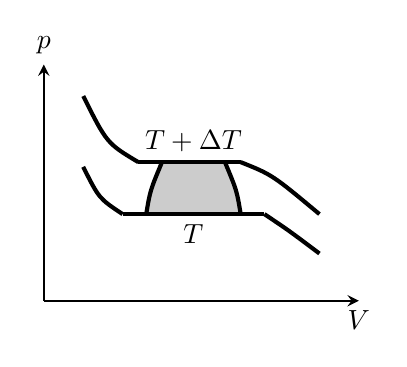
\begin{tikzpicture}[>=stealth, thick]
    % Axes
    \draw[->] (0, 0) -- (4, 0) node[below] {$V$};
    \draw[->] (0, 0) -- (0, 3) node[above] {$p$};
    
    % Shaded Region
    \fill[gray!40] (1.3, 1.1) .. controls (1.35, 1.4) .. (1.5, 1.76) -- (2.3, 1.76) .. controls (2.45, 1.4) .. (2.5, 1.1) -- cycle;
    
    % Isotherm T + \Delta T
    \draw[line width=1.5pt] (0.5, 2.6) .. controls (0.8, 2.0) .. (1.2, 1.76);
    \draw[line width=1.5pt] (1.2, 1.76) -- (2.5, 1.76);
    \draw[line width=1.5pt] (2.5, 1.76) .. controls (2.9, 1.6) .. (3.5, 1.1);
    \node[above] at (1.9, 1.76) {$T+\Delta T$};
    
    % Isotherm T
    \draw[line width=1.5pt] (0.5, 1.7) .. controls (0.7, 1.3) .. (1.0, 1.1);
    \draw[line width=1.5pt] (1.0, 1.1) -- (2.8, 1.1);
    \draw[line width=1.5pt] (2.8, 1.1) .. controls (3.1, 0.9) .. (3.5, 0.6);
    \node[below] at (1.9, 1.1) {$T$};
    
    % Carnot cycle vertical boundaries
    \draw[line width=1.5pt] (1.3, 1.1) .. controls (1.35, 1.4) .. (1.5, 1.76);
    \draw[line width=1.5pt] (2.5, 1.1) .. controls (2.45, 1.4) .. (2.3, 1.76);
\end{tikzpicture}
\end{center}
\end{exercise}
\begin{solution}

\end{solution}

\begin{exercise}\label{ex:14.8}
氢的三相点温度为 $T = 14 \ \mathrm{K}$. 在这一点上，液氢的密度为 $71 \ \mathrm{kg/m^3}$，固氢的密度是 $81 \ \mathrm{kg/m^3}$. 液体的蒸气压由下式给出：
$$ \ln(p/\mathrm{Pa}) \approx 18.3 - \frac{122}{T/\mathrm{K}} - 0.3 \ln(T/\mathrm{K}) $$
而融化温度为
$$ \frac{T_m}{\mathrm{K}} = 14 + \frac{1}{33} \frac{p}{101325 \ \mathrm{Pa}} $$
\begin{enumerate}
  \item[(a)] 计算 3 个潜热在三相点的数值. 用 $R$ 表示，精确到 $5\%$.
  \item[(b)] 计算三相点上固体曲线的斜率.
\end{enumerate}
\end{exercise}
\begin{solution}

\end{solution}

\begin{exercise}\label{ex:14.9}
在一级相变过程中证明：
\begin{enumerate}
  \item[(a)] 整个系统的熵变是总体积的线性函数；
  \item[(b)] 能量变化是
  $$ \Delta U = L \left( 1 - \frac{\mathrm{d}\ln T}{\mathrm{d}\ln p} \right) $$
\end{enumerate}
\end{exercise}
\begin{solution}

\end{solution}

\begin{exercise}\label{ex:14.10}
超导-正常相变的边界可由临界磁场公式来表达：
$$ H_c(T) = H_c(0)\left[ 1 - \left(\frac{T}{T_c}\right)^2 \right] $$
利用自由能的微分表达式
$$ \mathrm{d}G_m(T, H) = -S_m \mathrm{d}T - B \mathrm{d}H $$
其中 $B$、$H$ 分别为磁感应强度和磁场强度，求沿相界的熵差、潜热. 试对潜热加以讨论.
\end{exercise}
\begin{solution}

\end{solution}

\begin{exercise}\label{ex:14.11}
范德瓦耳斯气体有气液相变. 范德瓦耳斯等温线的麦克斯韦结构可以表达为
\begin{align}
  \int_{V_L}^{V_G} p(T,V) \mathrm{d}V &= p(V_G - V_L) \tag{1} \\
  p(V_G) &= p(V_L) \tag{2}
\end{align}
证明：利用约化变量
$$ \varepsilon = \frac{T}{T_C} - 1, \quad v = \frac{V}{V_C} - 1 $$
(1)式和(2)式可分别写为
\begin{align}
  \Delta \{ 4\varepsilon v - 4\varepsilon v^2 + v^3 \} &= 0 \tag{3} \\
  \Delta \{ 4\varepsilon v - 6\varepsilon v^2 + v^3 \} &= 0 \tag{4}
\end{align}
式中 $\Delta$ 表示对汽液两相的值求差. 注意到 $v_G > 0, v_L < 0$，实际上(3)式和(4)式给出了范德瓦耳斯气体的一个临界指数：$\beta = 1/2$.
\end{exercise}
\begin{solution}

\end{solution}
\chapter{第十五章 静电场}

1. 离 $4q$ 电荷 $\frac{2}{3}d$ ; $-\frac{4}{9}q$

5. $E_x = -\frac{1}{4\pi\varepsilon_0} \frac{\lambda}{R}$
$E_y = \frac{1}{4\pi\varepsilon_0} \frac{\lambda}{R}$

7. (a) $qQ / (4\pi\varepsilon_0 T)$ , (b) $\sqrt{T/m}$

9. $E(x) = \frac{ea}{8\varepsilon_0} \left( x_m^2 - 4x^2 \right)$

11. (a) $3.0 \times 10^3\text{N}$, (b) $240\text{MeV}$

13. $\frac{Q^2}{32\pi\varepsilon_0 R^2}$

15. (a) $V_P = \frac{k}{4\pi\varepsilon_0} \left( \sqrt{L^2 + y^2} - y \right)$
(b) $E_y = \frac{k}{4\pi\varepsilon_0} \left( 1 - \frac{y}{\sqrt{L^2 + y^2}} \right)$

17. $E_2 = \frac{\sigma}{3\varepsilon_0} ; \quad E_1 = \frac{2\sigma}{3\varepsilon_0}$

\begin{exercise}\label{ex:15.1}
两个自由点电荷分别带电 $q$ 和 $4q$，相距 $d$. 若放入第三个点电荷并使整个系统保持平衡，求第三个点电荷的位置和所带的电荷量. 该系统的平衡是稳定的吗？
\end{exercise}
\begin{solution}

\end{solution}

\begin{exercise}\label{ex:15.2}
粗略估计一杯水中所有正电荷的电荷量. 设一杯水的体积为 $250 \ \mathrm{cm^3}$.
\end{exercise}
\begin{solution}

\end{solution}

\begin{exercise}\label{ex:15.3}
如图，一种典型的电四极子是由两个电偶极子组成，试证明在轴线上距中心 $r$(设 $r \gg a$) 的 $P$ 点的电场强度为
$$ E = \frac{3Q}{4\pi\varepsilon_0 r^4} $$
式中 $Q = 2qa^2$ 称为电荷分布的电四极矩.
\begin{center}
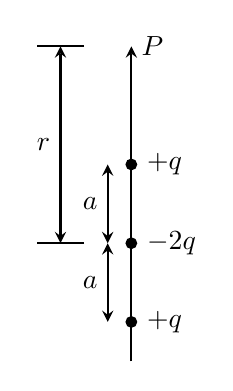
\begin{tikzpicture}[>=stealth, thick]
    % Axis line
    \draw (0, -1.5) -- (0, 2);
    \draw[->] (0, 2) -- (0, 2.5);
    \node[right] at (0, 2.5) {$P$};
    
    % Charges
    \filldraw[black] (0, 1) circle (0.06) node[right=2pt] {$+q$};
    \filldraw[black] (0, 0) circle (0.06) node[right=2pt] {$-2q$};
    \filldraw[black] (0, -1) circle (0.06) node[right=2pt] {$+q$};
    
    % Distances
    \draw[<->] (-0.3, 0) -- (-0.3, 1) node[midway, left] {$a$};
    \draw[<->] (-0.3, 0) -- (-0.3, -1) node[midway, left] {$a$};
    
    % Distance r (from center to P)
    \draw (-0.6, 0) -- (-1.2, 0);
    \draw (-0.6, 2.5) -- (-1.2, 2.5);
    \draw[<->] (-0.9, 0) -- (-0.9, 2.5) node[midway, left] {$r$};
\end{tikzpicture}
\end{center}
\end{exercise}
\begin{solution}

\end{solution}

\begin{exercise}\label{ex:15.4}
一个立方形的导体有 5 个面接地，而第 6 个面与其余 5 个面绝缘，电势为 $\phi_0$，问立方体中心的电势是多少？
\end{exercise}
\begin{solution}

\end{solution}

\begin{exercise}\label{ex:15.5}
如图所示，一根半无限长的绝缘棒均匀带电，电荷线密度为 $\lambda$. 试求图中 $P$ 点的电场强度的大小及方向.
\begin{center}
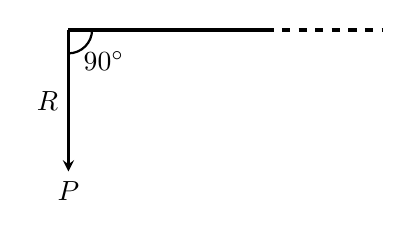
\begin{tikzpicture}[>=stealth, thick]
    % Horizontal Rod
    \draw[line width=1.5pt] (0, 2) -- (2.5, 2);
    \draw[line width=1.5pt, dashed] (2.5, 2) -- (4, 2);
    
    % Line to P
    \draw[->] (0, 2) -- (0, 0.2);
    \node[below] at (0, 0.2) {$P$};
    \node[left] at (0, 1.1) {$R$};
    
    % Angle
    \draw (0.3, 2) arc (0:-90:0.3);
    \node at (0.45, 1.6) {$90^\circ$};
\end{tikzpicture}
\end{center}
\end{exercise}
\begin{solution}

\end{solution}

\begin{exercise}\label{ex:15.6}
一根细玻璃棒弯成半径为 $R$ 的半圆形，等量的正负电荷 $+Q$ 与 $-Q$ 分别均匀地分布在玻璃棒的上下两部分(如图). 求圆心 $P$ 处的电场强度 $E$.
\begin{center}
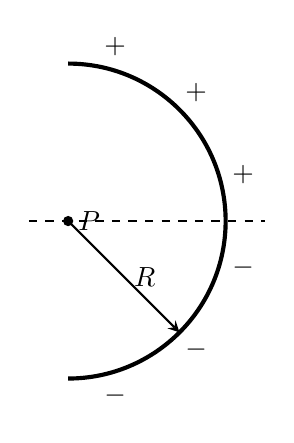
\begin{tikzpicture}[>=stealth, thick]
    \def\R{2}
    % Arc
    \draw[line width=1.5pt] (0,\R) arc (90:-90:\R);
    % P
    \filldraw[black] (0,0) circle (0.05) node[right] {$P$};
    % R
    \draw[->] (0,0) -- (-45:\R) node[midway, right] {$R$};
    % Signs
    \foreach \a in {15, 45, 75} {
        \node at (\a:\R+0.3) {$+$};
    }
    \foreach \a in {-15, -45, -75} {
        \node at (\a:\R+0.3) {$-$};
    }
    % Dashed line
    \draw[dashed] (-0.5, 0) -- (\R+0.5, 0);
\end{tikzpicture}
\end{center}
\end{exercise}
\begin{solution}

\end{solution}

\begin{exercise}\label{ex:15.7}
一质量为 $m$、带电 $q>0$ 的粒子具有初动能 $T$，从无穷远处向一个带电量为 $Q$ 的重原子核运动，设该原子核在我们的实验室参照系中是固定的.
\begin{enumerate}
  \item[(a)] 如果带电粒子很精确地正对着原子核运动，则粒子与核的最近距离是多少？
  \item[(b)] 若粒子的运动与(a)中相比有所偏离，且粒子与核的最近距离为(a)中结果的两倍，求粒子在最近处的速度大小.
\end{enumerate}
\end{exercise}
\begin{solution}

\end{solution}

\begin{exercise}\label{ex:15.8}
如图所示，质量为 $m = 1.0 \times 10^{-3} \ \mathrm{g}$ 的小圆球带有电量 $2.0 \times 10^{-8} \ \mathrm{C}$. 用丝线将它悬挂在一块垂直放置的大绝缘带电板上，丝线与板的夹角为 $\theta$. 试计算板上的电荷面密度 $\sigma$.
\begin{center}
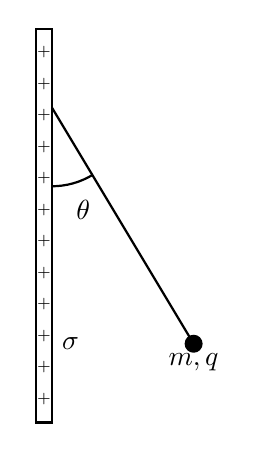
\begin{tikzpicture}[>=stealth, thick]
    % Plate
    \draw (0, -2.5) rectangle (0.2, 2.5);
    \foreach \y in {-2.2, -1.8, ..., 2.2} {
        \node at (0.1, \y) {\tiny $+$};
    }
    \node[right] at (0.2, -1.5) {$\sigma$};
    
    % Pendulum
    \draw (0.2, 1.5) -- (2, -1.5);
    \filldraw[black] (2, -1.5) circle (0.1) node[below] {$m,q$};
    
    % Angle
    \draw[dashed] (0.2, 1.5) -- (0.2, -1);
    \draw (0.2, 0.5) arc (270:301:1);
    \node at (0.6, 0.2) {$\theta$};
\end{tikzpicture}
\end{center}
\end{exercise}
\begin{solution}

\end{solution}

\begin{exercise}\label{ex:15.9}
求具有相等厚度 $0.5x_m$ 反型层而电荷密度为 $\rho(x) = -eax$ 的 p-n 结的电场. $a$ 是常量.
\end{exercise}
\begin{solution}

\end{solution}

\begin{exercise}\label{ex:15.10}
求电荷密度为 $\rho = ax\theta(x)\theta(d-x)$ 的无限大电荷板的电场. $a$、$d$ 是常量，$\theta$ 为阶梯函数：
$$ \theta(x) = \begin{cases} 0, & x < 0 \\ 1, & x > 0 \end{cases} $$
\end{exercise}
\begin{solution}

\end{solution}

\begin{exercise}\label{ex:15.11}
图中所示为 $^{235}\mathrm{U}$ 裂变时的理想化模型. 假设两裂片体积相等，带电量相同；并假设原先 $^{235}\mathrm{U}$ 的半径为 $8.0 \times 10^{-15} \ \mathrm{m}$，原子核的组分具有相同的密度. 
\begin{enumerate}
  \item[(a)] 计算两个裂片之间的相互排斥力；
  \item[(b)] 求两个裂片间的相互作用能.
\end{enumerate}
\begin{center}
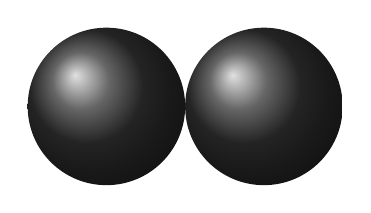
\begin{tikzpicture}[>=stealth, thick]
    \shade[ball color=black!80] (0,0) circle (1);
    \shade[ball color=black!80] (2,0) circle (1);
\end{tikzpicture}
\end{center}
\end{exercise}
\begin{solution}

\end{solution}

\begin{exercise}\label{ex:15.12}
电荷 $Q$ 均匀分布在半径为 $r$ 的球面上. 证明：带有电荷 $\mathrm{d}q$ 的小面元所受到的力径向向外，并由公式 $\mathrm{d}F = E\mathrm{d}q/2$ 给出，其中 $E$ 为球面上的电场强度.
\end{exercise}
\begin{solution}

\end{solution}

\begin{exercise}\label{ex:15.13}
一个带总电荷 $Q$、半径为 $R$ 的导体球被切成两半，若要保持两半球还在一起来，需要多大的力？
\end{exercise}
\begin{solution}

\end{solution}

\begin{exercise}\label{ex:15.14}
给一半径为 $R_0$ 的肥皂泡缓慢充以电荷 $q$. 由于表面电荷的互相排斥，肥皂泡的半径将略微增大至 $R$. 设大气压为 $p$，肥皂泡初始的体积为 $V_0$，则体积膨胀至 $V$ 时，泡内压强将降为 $p(V_0/V)$. 证明：
$$ q^2 = 32\pi^2\varepsilon_0 pR(R^3 - R_0^3) $$
\end{exercise}
\begin{solution}

\end{solution}

\begin{exercise}\label{ex:15.15}
如图，长度为 $L$ 的细棒水平放置在 $x$ 轴上，其一端正位于原点($x = 0$)，棒上电荷分布的线密度为 $\lambda = kx$，其中 $k$ 为常量. 
\begin{enumerate}
  \item[(a)] 设无穷远处的静电势为零，求 $y$ 轴上一点 $P$ 的电势. 
  \item[(b)] 由(a)的结果计算 $P$ 点场强的竖直分量 $E_y$；再利用积分的方法直接计算其结果. 
  \item[(c)] 为什么 $P$ 点场强的水平分量 $E_x$ 不能由(a)的结果求导得到呢？
\end{enumerate}
\begin{center}
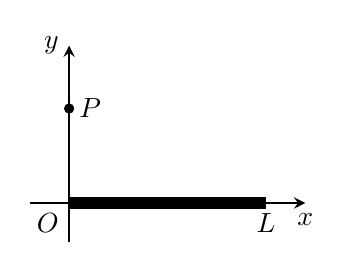
\begin{tikzpicture}[>=stealth, thick]
    % Axes
    \draw[->] (-0.5, 0) -- (3, 0) node[below] {$x$};
    \draw[->] (0, -0.5) -- (0, 2) node[left] {$y$};
    \node[below left] at (0,0) {$O$};
    
    % Rod
    \draw[line width=4pt] (0,0) -- (2.5, 0);
    \node[below] at (2.5, 0) {$L$};
    
    % Point P
    \filldraw[black] (0, 1.2) circle (0.05) node[right] {$P$};
\end{tikzpicture}
\end{center}
\end{exercise}
\begin{solution}

\end{solution}

\begin{exercise}\label{ex:15.16}
在两个半径分别为 $r_1$ 和 $r_2$ ($r_1 < r_2$) 的同心球之间填有电荷密度为 $\rho$ 的绝缘物质. 求距球心 $r$ 处的电势. 分别考虑：(a) $r > r_2$, (b) $r_2 > r > r_1$, (c) $r < r_1$. (d)在 $r = r_1$ 和 $r = r_2$ 处电势连续吗？
\end{exercise}
\begin{solution}

\end{solution}

\begin{exercise}\label{ex:15.17}
如图，两块大的金属平板，彼此相距为 $d$，它们的一个末端由一金属带连接. 有一塑料薄片，电荷面密度为 $\sigma$，置于两金属板之间，与上板距离为 $d/3$. 试求靠近上板和下板的电场 $\boldsymbol{E}_1$ 和 $\boldsymbol{E}_2$.
\begin{center}
\begin{tikzpicture}[>=stealth, thick]
    % Top plate
    \draw[line width=2pt] (0, 2) -- (4, 2);
    % Bottom plate
    \draw[line width=2pt] (0, 0) -- (4, 0);
    % Sheet
    \draw[line width=1pt] (0, 1.33) -- (4, 1.33);
    \node[below] at (3.5, 1.33) {$\sigma$};
    
    % Distances
    \draw[<->] (0.2, 1.33) -- (0.2, 2) node[midway, right] {$d/3$};
    \draw[<->] (0.2, 0) -- (0.2, 1.33) node[midway, right] {$2d/3$};
    
    % E fields
    \node at (2, 1.66) {$E_1$};
    \node at (2, 0.66) {$E_2$};
    
    % Metal band
    \draw[line width=1.5pt] (4, 2) arc (90:-90:0.5 and 1);
    \node[right] at (4.5, 1) {金属带};
\end{tikzpicture}
\end{center}
\end{exercise}
\begin{solution}

\end{solution}
\chapter{第十六章 导体和电介质}

1. $\frac{\varepsilon_0 A}{d}, \frac{\varepsilon_0 A}{d - b}$

5. 对 $\lambda = \text{const.} \quad \min R_1 = \frac{\lambda}{2\pi\varepsilon_0 E_b}$

7. $L \left( 1 - \frac{4\varepsilon_0 p_0 A^2}{Q^2} \right)^{1/2}$

9. (a) $8.9 \times 10^{-5}\text{J}$, (b) $2000\text{V}$

11. $-\frac{4\varepsilon_0 V_0}{9d^2} \sqrt{\frac{2eV_0}{m}}$

\begin{exercise}\label{ex:16.1}
如图，厚度为 $b$ 的铜片插入一平行板电容器中，铜片处于两平板的正中间. 求铜片插入前及插入后电容器的电容.
\begin{center}
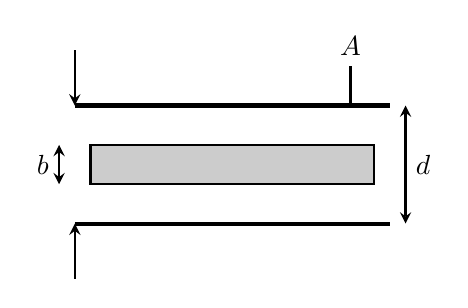
\begin{tikzpicture}[>=stealth, thick]
    % Plates
    \draw[line width=1.5pt] (0, 1.5) -- (4, 1.5);
    \draw[line width=1.5pt] (0, 0) -- (4, 0);
    
    % Copper block
    \fill[gray!40] (0.2, 0.5) rectangle (3.8, 1.0);
    \draw (0.2, 0.5) rectangle (3.8, 1.0);
    
    % Labels and dimensions
    \draw[<->] (4.2, 0) -- (4.2, 1.5) node[midway, right] {$d$};
    \draw[<->] (-0.2, 0.5) -- (-0.2, 1.0) node[midway, left] {$b$};
    
    % A label
    \draw (3.5, 1.5) -- (3.5, 2.0);
    \node[above] at (3.5, 2.0) {$A$};
    
    % Wires
    \draw[<-] (0, 1.5) -- (0, 2.2);
    \draw[<-] (0, 0) -- (0, -0.7);
\end{tikzpicture}
\end{center}
\end{exercise}
\begin{solution}

\end{solution}

\begin{exercise}\label{ex:16.2}
求图中 $x$ 与 $y$ 间的等效电容. 假设电容 $C_2$ 为 $10 \ \mu\mathrm{F}$，且其他电容均为 $4.0 \ \mu\mathrm{F}$.
\begin{center}
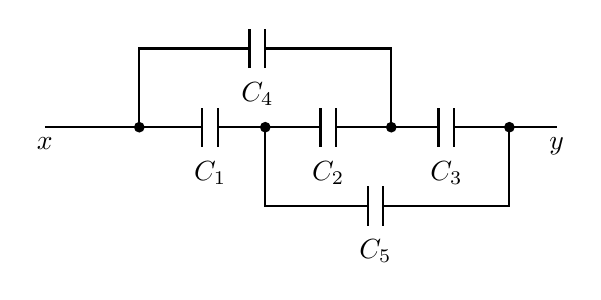
\begin{tikzpicture}[>=stealth, thick]
    % Nodes
    \draw (0,0) node[below] {$x$} -- (1.5,0);
    
    % C1
    \draw (1.5,0) -- (2,0);
    \draw (2,-0.25) -- (2,0.25);
    \draw (2.2,-0.25) -- (2.2,0.25);
    \node[below] at (2.1,-0.3) {$C_1$};
    \draw (2.2,0) -- (3.5,0);
    
    % C2
    \draw (3.5,-0.25) -- (3.5,0.25);
    \draw (3.7,-0.25) -- (3.7,0.25);
    \node[below] at (3.6,-0.3) {$C_2$};
    \draw (3.7,0) -- (5,0);
    
    % C3
    \draw (5,-0.25) -- (5,0.25);
    \draw (5.2,-0.25) -- (5.2,0.25);
    \node[below] at (5.1,-0.3) {$C_3$};
    \draw (5.2,0) -- (6.5,0) node[below] {$y$};
    
    % C4
    \draw (1.2,0) -- (1.2,1) -- (2.6,1);
    \draw (2.6,0.75) -- (2.6,1.25);
    \draw (2.8,0.75) -- (2.8,1.25);
    \node[below] at (2.7,0.7) {$C_4$};
    \draw (2.8,1) -- (4.4,1) -- (4.4,0);
    
    % C5
    \draw (2.8,0) -- (2.8,-1) -- (4.1,-1);
    \draw (4.1,-0.75) -- (4.1,-1.25);
    \draw (4.3,-0.75) -- (4.3,-1.25);
    \node[below] at (4.2,-1.3) {$C_5$};
    \draw (4.3,-1) -- (5.9,-1) -- (5.9,0);
    
    % Junction dots
    \filldraw (1.2,0) circle (1.5pt);
    \filldraw (2.8,0) circle (1.5pt);
    \filldraw (4.4,0) circle (1.5pt);
    \filldraw (5.9,0) circle (1.5pt);
\end{tikzpicture}
\end{center}
\end{exercise}
\begin{solution}

\end{solution}

\begin{exercise}\label{ex:16.3}
如图，一电容器的两平板均为边长为 $a$ 的正方形，但彼此形成一角度 $\theta$. 证明：当 $\theta$ 较小时，该电容器的电容由下式给出：
$$ C = \frac{\varepsilon_0 a^2}{d} \left( 1 - \frac{a\theta}{2d} \right) $$
\begin{center}
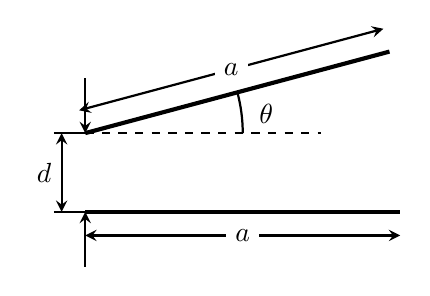
\begin{tikzpicture}[>=stealth, thick]
    % Bottom plate
    \draw[line width=1.5pt] (0, 0) -- (4, 0);
    \draw[<->] (0, -0.3) -- (4, -0.3) node[midway, fill=white] {$a$};
    
    % Top plate
    \begin{scope}[shift={(0, 1)}, rotate=15]
        \draw[line width=1.5pt] (0, 0) -- (4, 0);
        \draw[<->] (0, 0.3) -- (4, 0.3) node[midway, fill=white] {$a$};
    \end{scope}
    
    % Angle and dashed line
    \draw[dashed] (0,1) -- (3,1);
    \draw (2,1) arc (0:15:2);
    \node at (2.3, 1.25) {$\theta$};
    
    % Distance d
    \draw[<->] (-0.3, 0) -- (-0.3, 1) node[midway, left] {$d$};
    \draw (-0.4, 0) -- (0, 0);
    \draw (-0.4, 1) -- (0, 1);
    
    % Arrows for wires
    \draw[<-] (0, 1) -- (0, 1.7);
    \draw[<-] (0, 0) -- (0, -0.7);
\end{tikzpicture}
\end{center}
\end{exercise}
\begin{solution}

\end{solution}

\begin{exercise}\label{ex:16.4}
有一内半径为 $R$，外半径为 $R'$ 的柱形长电容器，试求单位长度上的电容. 若在外筒壁上有细微的凸起，试定性分析会产生什么结果.
\end{exercise}
\begin{solution}

\end{solution}

\begin{exercise}\label{ex:16.5}
由两同轴金属圆柱构成一空气电容器，内、外圆柱半径分别为 $R_1$、$R_2$.
\begin{enumerate}
  \item[(a)] 在大气介质不被击穿的前提下，应该如何选择内圆柱的半径以使两导体的电势差最大；
  \item[(b)] 在同样的前提下，应如何选择内半径以使电容器的贮能最大.
\end{enumerate}
\end{exercise}
\begin{solution}

\end{solution}

\begin{exercise}\label{ex:16.6}
已知两个平行板电极相距 $d$，电势分别为 $0$ 和 $V$. 两极板间充满电介质，其相对介电常数是距离的函数 $\varepsilon_{\mathrm{r}} = \mathrm{e}^{\alpha x}$. 求板间的电场 $E(x)$.
\end{exercise}
\begin{solution}

\end{solution}

\begin{exercise}\label{ex:16.7}
如图，一密封容器的两个相对的侧面是两块接地的导体，容器内有一竖直的面积为 $A$ 的导体隔板带有电荷 $Q$，该隔板与容器的其他部分是绝缘的，并且能不漏气地沿容器内壁无摩擦地滑动. 开始时隔板两边的空气的压强均为 $p_0$，求隔板处于平衡时的位置.
\begin{center}
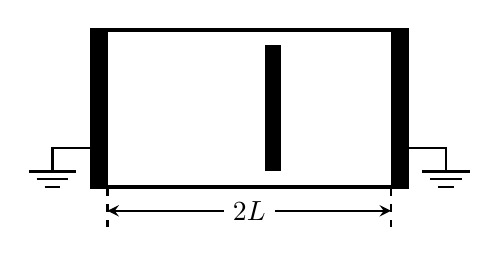
\begin{tikzpicture}[>=stealth, thick]
    % Container
    \draw[line width=1.5pt] (0, 0) rectangle (4, 2);
    
    % Grounded Plates (inner black blocks)
    \fill[black] (0, 0) rectangle (0.2, 2);
    \fill[black] (3.8, 0) rectangle (4, 2);
    
    % Movable Plate
    \fill[black] (2.2, 0.2) rectangle (2.4, 1.8);
    
    % Dimension 2L
    \draw[dashed] (0.2, 0) -- (0.2, -0.5);
    \draw[dashed] (3.8, 0) -- (3.8, -0.5);
    \draw[<->] (0.2, -0.3) -- (3.8, -0.3) node[midway, fill=white] {$2L$};
    
    % Left Ground
    \draw (0, 0.5) -- (-0.5, 0.5) -- (-0.5, 0.2);
    \draw (-0.8, 0.2) -- (-0.2, 0.2);
    \draw (-0.7, 0.1) -- (-0.3, 0.1);
    \draw (-0.6, 0.0) -- (-0.4, 0.0);
    
    % Right Ground
    \draw (4, 0.5) -- (4.5, 0.5) -- (4.5, 0.2);
    \draw (4.2, 0.2) -- (4.8, 0.2);
    \draw (4.3, 0.1) -- (4.7, 0.1);
    \draw (4.4, 0.0) -- (4.6, 0.0);
\end{tikzpicture}
\end{center}
\end{exercise}
\begin{solution}

\end{solution}

\begin{exercise}\label{ex:16.8}
两电容器并联连接，电容分别为 $2.0 \ \mu\mathrm{F}$ 和 $4.0 \ \mu\mathrm{F}$. 求加上 $300 \ \mathrm{V}$ 电势差时电容器内贮藏的能量.
\end{exercise}
\begin{solution}

\end{solution}

\begin{exercise}\label{ex:16.9}
已知一个平行板电容器，极板面积为 $0.20 \ \mathrm{m^2}$，间隙为 $1.0 \ \mathrm{cm}$，充电至 $1000 \ \mathrm{V}$ 后断开电源. 
\begin{enumerate}
  \item[(a)] 若把极板间隙拉开一倍，需要做多少功？
  \item[(b)] 电容器的终了电压是多少？
\end{enumerate}
\end{exercise}
\begin{solution}

\end{solution}

\begin{exercise}\label{ex:16.10}
厚度为 $b$，介电常数为 $\varepsilon_{\mathrm{r}}$ 的电介质置于平板电容器之间，平板面积为 $A$，两极板相距 $d$. 电介质插入前将电容器充电至电势差 $V_0$，然后便断开电源. 假设 $A = 100 \ \mathrm{cm^2}$，$d = 1.0 \ \mathrm{cm}$，$b = 0.50 \ \mathrm{cm}$，$\varepsilon_{\mathrm{r}} = 7.0$，$V_0 = 100 \ \mathrm{V}$. 
\begin{enumerate}
  \item[(a)] 计算介质板插入前的电容 $C_0$；
  \item[(b)] 计算极板上的自由电荷；
  \item[(c)] 分别计算极板间空气隙和介质中的电场强度；
  \item[(d)] 计算介质板插入后两极板间的电势差；
  \item[(e)] 有百分之几的电场能量储存在空气隙中？又有多少储存在介质板中？
\end{enumerate}
\end{exercise}
\begin{solution}

\end{solution}

\begin{exercise}\label{ex:16.11}
已知两个平行板电极相距 $d$，电势分别为 $0$ 和 $V_0$. 如果低电势的电极上有一电子源，电子从中由静止开始运动，忽略碰撞，求两极板间所流过的空间电流密度.
\end{exercise}
\begin{solution}

\end{solution}

\begin{exercise}\label{ex:16.12}
已知两个平行板电极相距 $d$，电势差为 $\Delta V$. 当部分地插入介电常量为 $\varepsilon$ 的电介质时，如图所示，
\begin{enumerate}
  \item[(a)] 求系统的静电能量；
  \item[(b)] 电介质所受的力.
\end{enumerate}
\begin{center}
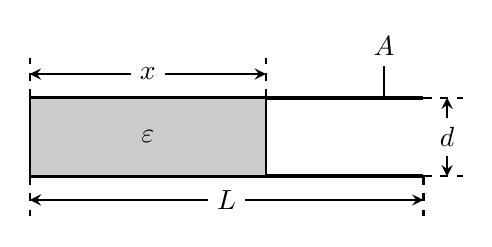
\begin{tikzpicture}[>=stealth, thick]
    % Plates
    \draw[line width=1.5pt] (0, 1) -- (5, 1);
    \draw[line width=1.5pt] (0, 0) -- (5, 0);
    
    % Dielectric
    \fill[gray!40] (0, 0) rectangle (3, 1);
    \draw (0,0) rectangle (3,1);
    \node at (1.5, 0.5) {$\varepsilon$};
    
    % Dimensions
    \draw[<->] (0, 1.3) -- (3, 1.3) node[midway, fill=white] {$x$};
    \draw[dashed] (0, 1) -- (0, 1.5);
    \draw[dashed] (3, 1) -- (3, 1.5);
    
    \draw[<->] (0, -0.3) -- (5, -0.3) node[midway, fill=white] {$L$};
    \draw[dashed] (0, 0) -- (0, -0.5);
    \draw[dashed] (5, 0) -- (5, -0.5);
    
    \draw[<->] (5.3, 0) -- (5.3, 1) node[midway, fill=white] {$d$};
    \draw[dashed] (5, 0) -- (5.5, 0);
    \draw[dashed] (5, 1) -- (5.5, 1);
    
    % A label
    \draw (4.5, 1) -- (4.5, 1.4);
    \node[above] at (4.5, 1.4) {$A$};
\end{tikzpicture}
\end{center}
\end{exercise}
\begin{solution}

\end{solution}
\chapter{第十七章 磁场}

1. $B = -\frac{\mu_0}{2} I \left( \frac{1}{R_1} - \frac{1}{R_2} \right) \mathbf{k}$

3. $B = \frac{2\sqrt{2}\mu_0 I}{\pi a}$

7. [图片：磁场或相关函数分布图]

9. (b) $T = \frac{2\pi}{\omega} = 3.57 \times 10^{-10}\text{s}$
$p = V_{||} T = 0.17\text{mm}$
$r = 1.5 \times 10^{-3}\text{m}$

11. 
$$T = \pi \sqrt{\frac{m}{(1+\alpha)k}}$$
$$\alpha = \frac{\sqrt{1 + \frac{\mu_0 I^2 L}{\pi k L_0^2}} - 1}{\sqrt{1 + \frac{\mu_0 I^2 L}{\pi k L_0^2}} + 1}$$

13. $dF = \frac{\omega}{2\pi}(QB + m\omega)Rd\varphi e_\rho$

\begin{exercise}\label{ex:17.1}
图中 $C$ 点为两半圆 $AD$ 和 $HJ$ 的共同圆心，两半圆半径分别为 $R_2$ 和 $R_1$，回路中通以电流 $I$，求 $C$ 点的磁感强度.
\begin{center}
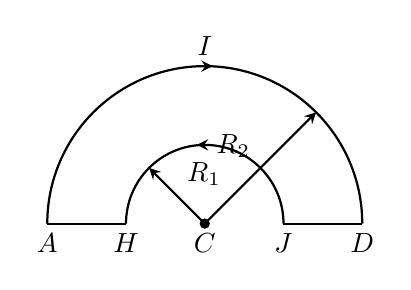
\begin{tikzpicture}[>=stealth, thick]
    \def\Rtwo{2}
    \def\Rone{1}
    
    % Outer arc AD
    \draw (-\Rtwo, 0) arc (180:0:\Rtwo);
    % Inner arc HJ
    \draw (\Rone, 0) arc (0:180:\Rone);
    
    % Straight segments
    \draw (-\Rtwo, 0) -- (-\Rone, 0);
    \draw (\Rone, 0) -- (\Rtwo, 0);
    
    % Nodes
    \node[below] at (-\Rtwo, 0) {$A$};
    \node[below] at (-\Rone, 0) {$H$};
    \node[below] at (\Rone, 0) {$J$};
    \node[below] at (\Rtwo, 0) {$D$};
    \filldraw[black] (0,0) circle (0.05) node[below] {$C$};
    
    % Current arrows
    \draw[->] (-0.1, \Rtwo) -- (0.1, \Rtwo);
    \node[above] at (0, \Rtwo) {$I$};
    \draw[->] (0.1, \Rone) -- (-0.1, \Rone);
    
    % Radius vectors
    \draw[->] (0,0) -- (45:\Rtwo) node[midway, above left] {$R_2$};
    \draw[->] (0,0) -- (135:\Rone) node[midway, above right] {$R_1$};
\end{tikzpicture}
\end{center}
\end{exercise}
\begin{solution}

\end{solution}

\begin{exercise}\label{ex:17.2}
亥姆霍兹线圈由两个完全相同的 $300$ 匝的圆形线圈构成，它们之间的距离恰好等于它们的半径(如图所示). 若 $R = 5.0 \ \mathrm{cm}$，$I = 50 \ \mathrm{A}$，
\begin{enumerate}
  \item[(a)] 画出磁感强度 $\boldsymbol{B}$ 在轴线上从 $x = -5.0 \ \mathrm{cm}$ 到 $x = 5.0 \ \mathrm{cm}$ 之间的变化情况，令 $P$ 点为 $x=0$ 的点；
  \item[(b)] 若两线圈间的距离 $z$ 为一变量，试证明：当 $z = R$ 时，不仅 $\mathrm{d}B/\mathrm{d}x$ 为零，$\mathrm{d}^2B/\mathrm{d}x^2$ 也为零.
\end{enumerate}
\begin{center}
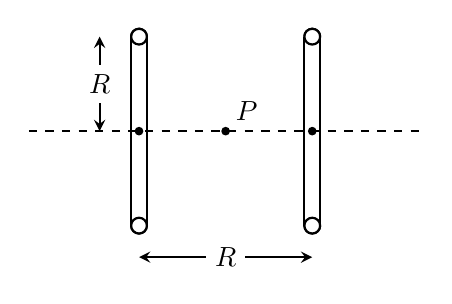
\begin{tikzpicture}[>=stealth, thick]
    % Axis
    \draw[dashed] (-2.5, 0) -- (2.5, 0);
    \filldraw[black] (0,0) circle (0.04) node[above right] {$P$};
    
    % Left coil
    \draw (-1.2, 1.2) -- (-1.2, -1.2);
    \draw (-1.0, 1.2) -- (-1.0, -1.2);
    \draw (-1.2, 1.2) arc (180:0:0.1);
    \draw (-1.2, -1.2) arc (180:360:0.1);
    \draw[fill=white] (-1.1, 1.2) circle (0.1);
    \draw[fill=white] (-1.1, -1.2) circle (0.1);
    
    % Right coil
    \draw (1.0, 1.2) -- (1.0, -1.2);
    \draw (1.2, 1.2) -- (1.2, -1.2);
    \draw (1.0, 1.2) arc (180:0:0.1);
    \draw (1.0, -1.2) arc (180:360:0.1);
    \draw[fill=white] (1.1, 1.2) circle (0.1);
    \draw[fill=white] (1.1, -1.2) circle (0.1);
    
    % Dimensions
    \draw[<->] (-1.1, -1.6) -- (1.1, -1.6) node[midway, fill=white] {$R$};
    \draw[<->] (-1.6, 0) -- (-1.6, 1.2) node[midway, fill=white] {$R$};
    
    % Centers
    \filldraw[black] (-1.1, 0) circle (0.04);
    \filldraw[black] (1.1, 0) circle (0.04);
\end{tikzpicture}
\end{center}
\end{exercise}
\begin{solution}

\end{solution}

\begin{exercise}\label{ex:17.3}
边长为 $a$ 的正方形线圈中通以电流 $I$，证明
\begin{enumerate}
  \item[(a)] 其中心处的磁感强度为
  $$ B = \frac{2\sqrt{2}\mu_0 I}{\pi a} $$
  \item[(b)] 该正方形的轴线上距中心 $x$ 处的磁感强度的大小为
  $$ B = \frac{4\mu_0 I a^2}{\pi(4x^2 + a^2)(4x^2 + 2a^2)^{1/2}} $$
\end{enumerate}
\end{exercise}
\begin{solution}

\end{solution}

\begin{exercise}\label{ex:17.4}
如图，抛物线形状的无穷长导线载有电流 $I$，焦点 $F$ 到顶点 $O$ 的距离为 $a$，试求焦点处的磁感强度 $\boldsymbol{B}$.
\begin{center}
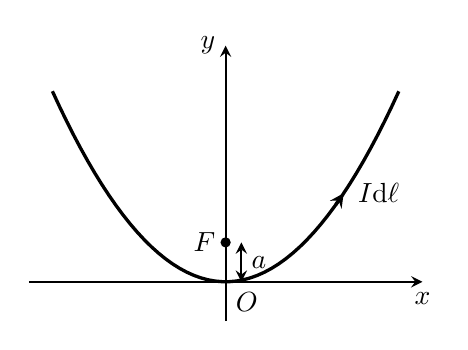
\begin{tikzpicture}[>=stealth, thick]
    % Axes
    \draw[->] (-2.5, 0) -- (2.5, 0) node[below] {$x$};
    \draw[->] (0, -0.5) -- (0, 3) node[left] {$y$};
    \node[below right] at (0,0) {$O$};
    
    % Parabola
    \draw[domain=-2.2:2.2, samples=50, line width=1.2pt] plot (\x, {0.5*\x*\x});
    
    % Focus
    \filldraw[black] (0, 0.5) circle (0.05) node[left] {$F$};
    
    % Distance a
    \draw[<->] (0.2, 0) -- (0.2, 0.5) node[midway, right] {$a$};
    
    % Current arrow
    \draw[->, line width=1.2pt] (1.4, {0.5*1.4*1.4}) -- (1.5, {0.5*1.5*1.5});
    \node[right] at (1.55, {0.5*1.5*1.5}) {$I\mathrm{d}\ell$};
\end{tikzpicture}
\end{center}
\end{exercise}
\begin{solution}

\end{solution}

\begin{exercise}\label{ex:17.5}
设定 $n$ 边形线圈的外接圆半径为 $R$，线圈中通以电流 $I$. 证明其中心处的磁感强度为
$$ B = \frac{\mu_0 n I}{2\pi a} \tan(\pi/n) $$
\end{exercise}
\begin{solution}

\end{solution}

\begin{exercise}\label{ex:17.6}
截面为 $5.0 \ \mathrm{cm} \times 5.0 \ \mathrm{cm}$、匝数为 $500$ 的螺绕环的内半径为 $15 \ \mathrm{cm}$，通以电流 $0.8 \ \mathrm{A}$. 
\begin{enumerate}
  \item[(a)] 在截面中心处(即距离圆心 $17.5 \ \mathrm{cm}$)的磁感强度 $\boldsymbol{B}$ 的大小是多少？
  \item[(b)] 通过螺绕环截面的磁通量是多少？
\end{enumerate}
\end{exercise}
\begin{solution}

\end{solution}

\begin{exercise}\label{ex:17.7}
内外半径分别为 $R$ 和 $R'$ 的中空圆柱中沿轴线方向通有均匀分布的电流 $I$. 
\begin{enumerate}
  \item[(a)] 证明圆柱截面上距圆心 $r(R < r < R')$ 处的磁感强度 $\boldsymbol{B}$ 为
  $$ B = \frac{\mu_0 I}{2\pi(R'^2 - R^2)} \frac{r^2 - R^2}{r} $$
  当 $R=0$ 时检验该结果；
  \item[(b)] 画出 $B$ 从 $r=0$ 到 $r \to \infty$ 的变化情形.
\end{enumerate}
\end{exercise}
\begin{solution}

\end{solution}

\begin{exercise}\label{ex:17.8}
两根相距 $d$ 的长直导线通以反向等量电流 $I$，如图所示，求与两导线距离相等的 $P$ 点的磁感强度的大小和方向.
\begin{center}
\begin{tikzpicture}[>=stealth, thick]
    % Top wire
    \filldraw[black] (0, 1) circle (0.15);
    \node[white] at (0, 1) {$\times$};
    \node[right] at (0.2, 1) {$I$};
    
    % Bottom wire
    \filldraw[black] (0, -1) circle (0.15);
    \node[white] at (0, -1) {$\cdot$};
    \node[right] at (0.2, -1) {$I$};
    
    % Distance d
    \draw[<->] (-0.4, -1) -- (-0.4, 1) node[midway, left] {$d$};
    
    % P and R
    \draw (0, 0) -- (2.5, 0);
    \filldraw[black] (2.5, 0) circle (0.05) node[right] {$P$};
    \node[above] at (1.25, 0) {$R$};
\end{tikzpicture}
\end{center}
\end{exercise}
\begin{solution}

\end{solution}

\begin{exercise}\label{ex:17.9}
$2.0 \ \mathrm{keV}$ 的正电子射入大小为 $0.10 \ \mathrm{T}$ 的匀强磁场 $\boldsymbol{B}$ 中，其速度方向与磁场 $\boldsymbol{B}$ 的夹角为 $89^\circ$. 
\begin{enumerate}
  \item[(a)] 证明正电子的路径为一螺旋线，其轴线沿 $\boldsymbol{B}$ 的方向. 
  \item[(b)] 求该螺旋线的周期、螺距以及半径.
\end{enumerate}
\end{exercise}
\begin{solution}

\end{solution}

\begin{exercise}\label{ex:17.10}
一束质量均为 $m$、电荷量均为 $q$ 的离子在点 $P$ 处以同一速率 $v$ 沿 $xy$ 上半平面中的各个方向射出. 垂直于 $xy$ 平面的均匀磁场 $\boldsymbol{B}$ 将这些离子聚焦于点 $R$，$R$ 与 $P$ 相距为 $2\rho$ ($\rho$ 为回转半径)，离子的轨道应该是轴对称的. 试确定磁场区的边界. 设离子间的相互作用可以忽略.
\end{exercise}
\begin{solution}

\end{solution}

\begin{exercise}\label{ex:17.11}
两根平行金属棒与金属弹簧构成回路，如图. 已知棒长为 $L$、质量为 $m$，系统只能作左右对称的运动，边缘效应可以忽略. 设弹簧的劲度系数为 $k$，原长为 $L_0$. 假设以某种方式使回路中有恒定的电流 $I$，且电磁感应可以忽略，试求两棒围绕平衡位置作小振动的周期.
\begin{center}
\begin{tikzpicture}[>=stealth, thick]
    % Top Spring
    \draw[decorate, decoration={coil, aspect=0.4, segment length=3mm, amplitude=3mm}] (-1.5, 1.5) -- (1.5, 1.5);
    \node[below] at (0, 1.2) {$k \quad L_0$};
    
    % Bottom Spring
    \draw[decorate, decoration={coil, aspect=0.4, segment length=3mm, amplitude=3mm}] (-1.5, -1.5) -- (1.5, -1.5);
    
    % Left Rod
    \draw[line width=3pt] (-1.5, -1.5) -- (-1.5, 1.5);
    \draw[->] (-1.8, -0.2) -- (-1.8, 0.2) node[left] {$I$};
    \node[right] at (-1.4, 0) {$L$};
    \node[right] at (-1.4, -0.3) {$m$};
    
    % Right Rod
    \draw[line width=3pt] (1.5, -1.5) -- (1.5, 1.5);
    \draw[->] (1.8, 0.2) -- (1.8, -0.2) node[right] {$I$};
    \node[right] at (1.6, 0) {$L$};
    \node[right] at (1.6, -0.3) {$m$};
\end{tikzpicture}
\end{center}
\end{exercise}
\begin{solution}

\end{solution}

\begin{exercise}\label{ex:17.12}
霍尔效应实验中，一长、宽、厚分别为 $4.0 \ \mathrm{cm}$、$1.0 \ \mathrm{cm}$、$1.0 \times 10^{-3} \ \mathrm{cm}$ 的导体置于强度为 $1.5 \ \mathrm{T}$ 的匀强磁场中，导体中沿长度方向通以 $3.0 \ \mathrm{A}$ 的电流，磁场垂直穿过导体，结果在横向方向产生 $1.0 \times 10^{-5} \ \mathrm{V}$ 的霍尔电势差. 由上述数据，
\begin{enumerate}
  \item[(a)] 计算导体中带电粒子的漂移速率；
  \item[(b)] 计算带电粒子的密度；
  \item[(c)] 作图表示导体上霍尔电势的极性分布(假设带电粒子为电子).
\end{enumerate}
\end{exercise}
\begin{solution}

\end{solution}

\begin{exercise}\label{ex:17.13}
如图所示半径为 $R$、质量为 $m$ 的匀质细圆环均匀带电，总电量为 $Q$ ($Q>0$)，放在光滑的水平桌面上. 环内外有垂直向上的均匀磁场 $\boldsymbol{B}$. 若将圆环以角速度 $\omega$ 绕着圆环的竖直轴匀速转动，试求环内因为这种转动而形成的附加张力.
\begin{center}
\begin{tikzpicture}[>=stealth, thick]
    % Ring
    \draw[line width=1.5pt] (0,0) ellipse (2 and 0.6);
    
    % Rotation axis
    \draw[dashed] (0, -1.5) -- (0, 1.5);
    \draw[->] (0, 1.5) -- (0, 2);
    
    % Omega arrow
    \draw[->] (-0.3, 1.2) arc (180:0:0.3 and 0.1);
    \node[above] at (0.4, 1.2) {$\omega$};
    
    % Radius
    \draw (0,0) -- (2,0);
    \node[above] at (1, 0) {$R$};
    
    % Labels
    \node[left] at (-2, 0) {$m$};
    \node[below left] at (-0.2, -0.6) {$Q$};
    
    % Magnetic field
    \draw[->] (-1.5, -1) -- (-1.5, 1);
    \draw[->] (1.5, -1) -- (1.5, 1);
    \node[right] at (1.5, 1) {$\boldsymbol{B}$};
\end{tikzpicture}
\end{center}
\end{exercise}
\begin{solution}

\end{solution}
\chapter{第十八章 电磁感应}

1. $\varepsilon = 1.5 \times 10^{-4}\text{V}$

3. 
$$I(t) = \frac{\pi r^2 N B \omega}{\sqrt{R^2 + L^2 \omega^2}} \sin(\omega t - \varphi)$$
$$M = \frac{(\pi r^2 N B)^2 \omega}{\sqrt{R^2 + L^2 \omega^2}} \sin\omega t \sin(\omega t - \varphi)$$
$$\left( \varphi = \arctan \frac{L\omega}{R} \right)$$

7. $T = \frac{\pi r_0^2 B^2}{RF}$

9. $B_{\perp} = RQ_1 / 2\ell_1\ell_2$
$B_{//} = RQ_2 / \ell_1\ell_2$

\begin{exercise}\label{ex:18.1}
图中表示一电阻为 $R$ 的铜棒沿两根平行的导电轨道运动，速度为 $v = 5.0 \ \mathrm{m/s}$. 轨道近旁有一平行的长直导线，通以电流 $I = 100 \ \mathrm{A}$，设 $a = 1.0 \ \mathrm{cm}$，$b = 20 \ \mathrm{cm}$. 计算铜棒中的感应电动势.
\begin{center}
\begin{tikzpicture}[>=stealth, thick]
    % Long wire
    \draw (0, 2) -- (4, 2);
    \draw[->] (3, 2) -- (3.5, 2) node[above] {$I$};
    
    % Rails
    \draw (0, 1) -- (4, 1);
    \draw (0, 0) -- (4, 0);
    
    % Resistor
    \draw (0, 1) -- (0, 0.7);
    \draw (0, 0.3) -- (0, 0);
    \draw (-0.15, 0.7) rectangle (0.15, 0.3);
    \node[left] at (-0.15, 0.5) {$R$};
    
    % Dimensions
    \draw[<->] (-0.5, 1) -- (-0.5, 2) node[midway, left] {$a$};
    \draw[dashed] (0, 1) -- (-0.6, 1);
    \draw[dashed] (0, 2) -- (-0.6, 2);
    
    \draw[<->] (-0.5, 0) -- (-0.5, 1) node[midway, left] {$b$};
    \draw[dashed] (0, 0) -- (-0.6, 0);
    
    % Rod
    \draw[line width=3pt] (2.5, -0.2) -- (2.5, 1.2);
    \draw[->] (2.6, 0.5) -- (3.2, 0.5) node[right] {$v$};
\end{tikzpicture}
\end{center}
\end{exercise}
\begin{solution}

\end{solution}

\begin{exercise}\label{ex:18.2}
设有一匀强磁场 $\boldsymbol{B}$ 分布在一半径为 $R$ 的柱形区域，并以速率 $\mathrm{d}B/\mathrm{d}t$ 变化. 长度为 $\ell$ 的金属棒按图中形式放置. 证明由此棒中产生的感应电动势由下式给出：
$$ \varepsilon = \frac{\mathrm{d}B}{\mathrm{d}t} \frac{\ell}{2} \sqrt{R^2 - \left(\frac{\ell}{2}\right)^2} $$
\begin{center}
\begin{tikzpicture}[>=stealth, thick]
    % Circle
    \draw (0,0) circle (2);
    
    % B field crosses
    \foreach \x/\y in {0/1.2, -1.2/0, 1.2/0, 0/-1.2, 1/1, -1/1, 1/-1, -1/-1, 0/0, 0.5/1.7, -0.5/1.7, 1.7/0.5, 1.7/-0.5, -1.7/0.5, -1.7/-0.5, -0.5/-1.7, 0.5/-1.7} {
        \node at (\x, \y) {$\times$};
    }
    
    % Rod
    \draw[line width=3pt] (-1.6, -1.2) -- (1.6, -1.2);
    
    % l label
    \draw[<->] (-1.6, -1.6) -- (1.6, -1.6) node[midway, fill=white] {$\ell$};
    \draw[dashed] (-1.6, -1.2) -- (-1.6, -1.7);
    \draw[dashed] (1.6, -1.2) -- (1.6, -1.7);
    
    % Radius R
    \draw[->] (0,0) -- (30:2) node[midway, above left] {$R$};
\end{tikzpicture}
\end{center}
\end{exercise}
\begin{solution}

\end{solution}

\begin{exercise}\label{ex:18.3}
一 $N$ 匝闭合线圈，半径为 $r$，电阻为 $R$，自感为 $L$，置于均匀磁场 $\boldsymbol{B}$ 中，该线圈绕一与 $\boldsymbol{B}$ 垂直的直径转动. 
\begin{enumerate}
  \item[(a)] 当线圈以常角速度 $\omega$ 转动时，求线圈中的电流与角度 $\theta$ 的函数关系. 这里 $\theta$ 是线圈平面的法向方向与 $\boldsymbol{B}$ 之间的夹角；
  \item[(b)] 为了维持上述转动，需加多大的外力矩 $M$？
\end{enumerate}
\end{exercise}
\begin{solution}

\end{solution}

\begin{exercise}\label{ex:18.4}
两根平行的长直导线(通以反向等量电流)中心相距 $d$，忽略通过导线自身的磁通量，证明在导线上长度为 $l$ 的部分的电感为
$$ L = \frac{\mu_0 l}{\pi} \ln \frac{d-r}{r} $$
其中 $r$ 是导线的半径.
\end{exercise}
\begin{solution}

\end{solution}

\begin{exercise}\label{ex:18.5}
设两同轴线圈 A、B，半径均为 $r$，相距为 $d$，电流 $I = k_0 t^2$ 通过线圈 A，而线圈 B 的电阻为 $R$. 证明：若自感可以忽略且 $r \ll d$，作用在线圈 B 上的力为
$$ \left(\frac{\mu_0}{4\pi}\right)^2 \frac{24\pi^4 r^8 k_0^2 t^3}{d^7 R} $$
并指出力的方向.
\end{exercise}
\begin{solution}

\end{solution}

\begin{exercise}\label{ex:18.6}
图中质量为 $m$ 的小珠可沿半径为 $r$ 的圆形轨道运动，环面为水平面. 小珠带有固定的正电荷 $q$. 设在以环形轨道为其正截面的柱体内有均匀的随时间 $t$ 变化的磁场，磁感应强度的方向垂直于环面. 已知 $t=0$ 时，$B=0$，小珠静止于环上；$0 < t < T$ 时，$B$ 随时间 $t$ 线性地增长；$t=T$ 时，$B=B_0$. 设重力和摩擦力可忽略. 试求：在 $0 \le t \le T$ 时间内小珠的运动状态及小珠对轨道的作用力.
\begin{center}
\begin{tikzpicture}[>=stealth, thick]
    % Circular track
    \draw (0,0) circle (2);
    
    % Bead
    \filldraw (45:2) circle (0.1) node[right] {$m$};
    \node[below right] at (45:2) {$q$};
    
    % Radius
    \draw[->] (0,0) -- (135:2) node[midway, below left] {$r$};
    
    % B field indication
    \draw (-1,-1) circle (0.3);
    \node at (-1,-1) {$\times$};
    \node[right] at (-0.6, -1) {$\boldsymbol{B}(t)$};
\end{tikzpicture}
\end{center}
\end{exercise}
\begin{solution}

\end{solution}

\begin{exercise}\label{ex:18.7}
图中 $ABCDA$ 是闭合导体回路，总电阻为 $R$，$AB$ 段的一部分变成初始半径为 $r_0$ 的小圆圈. 圆圈所在区域有与圆圈平面垂直的均匀磁场 $B_m$. 回路的 $B$ 端固定，$C$、$D$ 端为自由端. $A$ 端在沿 $BA$ 方向的恒力 $\boldsymbol{F}$ 的作用下向右移动，从而使圆圈缓慢缩小. 设在圆圈缩小的过程中，始终保持圆的形状，并设导体回路是柔软的，阻力可以忽略. 试求此圆圈从初始的半径 $r_0$ 到完全消失所需的时间 $T$.
\begin{center}
\begin{tikzpicture}[>=stealth, thick]
    % Main rectangle boundaries
    \draw (-2, 0) node[above right] {$C$} -- (2, 0) node[above left] {$D$};
    \draw (-2, 0) -- (-2, 2) node[above right] {$B$};
    \draw (2, 0) -- (2, 2);
    
    % Top wire parts
    \draw (-2, 2) -- (-0.5, 2);
    \draw (0.5, 2) -- (1.5, 2) node[above] {$A$};
    
    % Force F
    \draw[->, line width=1.5pt] (1.5, 2) -- (2.5, 2) node[right] {$\boldsymbol{F}$};
    
    % Loop
    \draw (0, 1.2) circle (0.8);
    \draw (-0.5, 2) -- (-0.4, 1.89);
    \draw (0.5, 2) -- (0.4, 1.89);
    
    % Center and Bm
    \filldraw (0, 1.2) circle (0.05);
    \draw (0, 0.8) circle (0.2);
    \filldraw (0, 0.8) circle (0.04);
    \node[right] at (0.2, 0.8) {$B_m$};
    
    % r0
    \draw[->] (0, 1.2) -- (0.8, 1.2) node[midway, above] {$r_0$};
\end{tikzpicture}
\end{center}
\end{exercise}
\begin{solution}

\end{solution}

\begin{exercise}\label{ex:18.8}
如图所示，在一半径为 $R$，质量为 $m$，可以无摩擦地自由转动的匀质绝缘盘中部装有一细长螺线管，其半径为 $r$，单位长度上绕有 $n$ 匝线圈，线圈中通以稳恒电流 $I$. 在圆盘的边缘上均匀地嵌着 $N$ 个正电荷 $q$. 设开始时螺线管中的电流为 $I$，圆盘静止，然后将电流切断. 试求圆盘转动的角速度.
\begin{center}
\begin{tikzpicture}[>=stealth, thick]
    % Disc
    \draw (0,0) ellipse (2.5 and 0.8);
    \draw (0,-0.8) arc (270:360:2.5 and 0.8);
    
    % Charges
    \foreach \a in {0, 30, 60, 90, 120, 150, 180, 210, 240, 270, 300, 330} {
        \filldraw (\a:2.5 and 0.8) circle (0.04);
    }
    \node[right] at (2.5, 0) {$q$};
    
    % Solenoid
    \draw (-0.5, 1.5) -- (-0.5, -1.5);
    \draw (0.5, 1.5) -- (0.5, -1.5);
    \draw (0, 1.5) ellipse (0.5 and 0.15);
    \draw (-0.5, -1.5) arc (180:360:0.5 and 0.15);
    \draw[dashed] (0.5, -1.5) arc (0:180:0.5 and 0.15);
    
    % Windings
    \foreach \y in {-1.2, -0.9, -0.6, -0.3, 0, 0.3, 0.6, 0.9, 1.2} {
        \draw (-0.5, \y) arc (180:360:0.5 and 0.08);
    }
    
    % Current and dimensions
    \draw[->] (0.5, 0.5) -- (1.0, 0.5) node[right] {$I$};
    \draw[->] (0,0) -- (-1.8, -0.55) node[midway, below] {$R$};
\end{tikzpicture}
\end{center}
\end{exercise}
\begin{solution}

\end{solution}

\begin{exercise}\label{ex:18.9}
如图所示，在水平桌面上平放着长方形线圈 $abcd$，已知 $ab$ 边长 $l_1$，$bc$ 边长 $l_2$，线圈总电阻为 $R$，$ab$ 边正好指向北方. 现将线圈以南北方向为轴翻转 $180^\circ$，使 $ab$ 与 $cd$ 互换位置，在翻转过程中测得通过导线的总电量为 $Q_1$. 然后，维持 $ad$ 边(东西方向)不动，将线圈绕 $ad$ 边转动 $90^\circ$，使之竖直，测得在竖直过程中流过导线的总电量为 $Q_2$. 试求该处地磁场 $\boldsymbol{B}$ 的大小.
\begin{center}
\begin{tikzpicture}[>=stealth, thick]
    % Parallelogram
    \draw (0, 0) node[left] {$a$} -- (2, -0.5) node[right] {$d$} -- (3, 3) node[right] {$c$} -- (1, 3.5) node[left] {$b$} -- cycle;
    
    % Labels
    \node[left] at (0.5, 1.75) {$\ell_1$};
    \node[below right] at (2.5, 1.25) {$\ell_2$};
\end{tikzpicture}
\end{center}
\end{exercise}
\begin{solution}

\end{solution}

\begin{exercise}\label{ex:18.10}
由半径为 $1.0 \ \mathrm{mm}$ 的导线构成的半径为 $10 \ \mathrm{cm}$ 的圆形线圈处于超导状态. 开始时线圈内通有 $100 \ \mathrm{A}$ 的电流. 一年后测出线圈内电流的减小量不足 $10^{-6} \ \mathrm{A}$. 试粗略估计此线圈电阻率的上限.
\end{exercise}
\begin{solution}

\end{solution}

\begin{exercise}\label{ex:18.11}
一圆柱金属块放在高频感应炉中加热(如图). 设感应炉的线圈产生的磁场是均匀的，磁感应强度的方均根值为 $B$，频率为 $f$. 金属圆柱的直径为 $D$，高为 $h$，电导率为 $\sigma$，柱轴与磁场平行. 设涡电流产生的磁场可以忽略. 试证明在金属圆柱内因涡电流产生的平均热功率为
$$ \overline{P} = \frac{1}{32} \pi^3 f^2 \sigma B^2 D^4 h $$
\begin{center}
\begin{tikzpicture}[>=stealth, thick]
    % Cylinder
    \draw (-1, -1.5) -- (-1, 1.5);
    \draw (1, -1.5) -- (1, 1.5);
    \draw (0, 1.5) ellipse (1 and 0.2);
    \draw (-1, -1.5) arc (180:360:1 and 0.2);
    
    % Coil
    \foreach \y in {-1.8, -1.4, -1.0, -0.6, -0.2, 0.2, 0.6, 1.0, 1.4, 1.8} {
        \draw (-1.2, \y) arc (180:360:1.2 and 0.2);
    }
    \draw (-1.2, -1.8) -- (-1.2, -2.5) -- (-1.6, -2.5);
    \draw (-1.2, 1.8) -- (-1.2, 2.5) -- (-1.6, 2.5);
    
    % AC source
    \draw (-1.6, 0) circle (0.3);
    \draw (-1.8, 0) .. controls (-1.7, 0.2) and (-1.5, -0.2) .. (-1.4, 0);
    \draw (-1.6, 0.3) -- (-1.6, 2.5);
    \draw (-1.6, -0.3) -- (-1.6, -2.5);
\end{tikzpicture}
\end{center}
\end{exercise}
\begin{solution}

\end{solution}
\chapter{第十九章 物质的磁性}

1. $\mu = e \frac{\omega}{2\pi} \pi \rho^2$
$\Delta \mu = -\frac{1}{4m} e^2 \rho^2 B$
$\rho = 0.64 \times 10^{-10} \text{m} = 0.064 \text{nm}$

3. $1.4 \times 10^{-3}\text{K}$

5. $L = \frac{2}{5} mr^2 \omega$
$\mu = \frac{1}{5} Q\omega R^2$
$\frac{Q}{2m}$

7. $5.15 \times 10^{-24}\text{J/T}$

9. $\frac{H_0 \cdot 2\pi R_1}{I}$
$M = \frac{B_0}{\mu_0}$

\begin{exercise}\label{ex:19.1}
一原子被置于磁场 $\boldsymbol{B}$ 中. 原子中的电子作半径为 $\rho$ 和频率为 $\omega$ 的圆周运动，轨道平面与 $\boldsymbol{B}$ 垂直. 
\begin{enumerate}
  \item[(a)] 求不存在磁场时原子的磁矩；
  \item[(b)] 求存在磁场时原子的磁矩；
  \item[(c)] 如果材料的原子数密度为 $2.8 \times 10^{28} \ \mathrm{/m^3}$，磁化率为 $-10^{-6}$，求原子的半径.
\end{enumerate}
\end{exercise}
\begin{solution}

\end{solution}

\begin{exercise}\label{ex:19.2}
如上题. 如果另有一电子在同样的轨道上以同样的频率反方向运动，求有磁场和无磁场时原子的磁矩.
\end{exercise}
\begin{solution}

\end{solution}

\begin{exercise}\label{ex:19.3}
石蜡包含很多质子. 质子自旋为 $1/2$，磁矩为 $1.4 \times 10^{-26} \ \mathrm{J/T}$. 石蜡置于 $3 \ \mathrm{T}$ 的磁场中. 为了使 $75\%$ 的质子的自旋与外场平行，温度应该是多少？
\end{exercise}
\begin{solution}

\end{solution}

\begin{exercise}\label{ex:19.4}
半径为 $r$ 的介电圆环上均匀分布有电荷 $Q$. 求圆环绕通过中心、垂直环面的轴以角速度 $\omega$ 旋转时的磁矩.
\end{exercise}
\begin{solution}

\end{solution}

\begin{exercise}\label{ex:19.5}
半径为 $r$、质量为 $m$ 的介电球上均匀分布有电荷 $Q$. 求当它绕通过球心的轴旋转时的自旋角动量和磁矩以及它们之比.
\end{exercise}
\begin{solution}

\end{solution}

\begin{exercise}\label{ex:19.6}
电子自旋磁矩为 $9.285 \times 10^{-24} \ \mathrm{J/T}$. 在 $1 \ \mathrm{T}$ 的磁场中，磁矩反平行和平行时磁能的差是多少？相当于这一能量的热能对应的温度是多少？
\end{exercise}
\begin{solution}

\end{solution}

\begin{exercise}\label{ex:19.7}
铁磁金属镍的饱和磁化强度是 $4.7 \times 10^5 \ \mathrm{A/m}$. 镍的原子量是 $58.71$，密度是 $8.90 \ \mathrm{g/cm^3}$. 试计算单个镍原子的磁矩.
\end{exercise}
\begin{solution}

\end{solution}

\begin{exercise}\label{ex:19.8}
在居里温度以上，金属钆 $\mathrm{Gd(gadolinium)}$ 的磁化率的倒数有如下数值：温度 $600 \ \mathrm{K}$ 时，为 $5.82 \times 10^3$，$1000 \ \mathrm{K}$ 时，为 $1.35 \times 10^4$. 
\begin{enumerate}
  \item[(a)] 求居里温度. 
  \item[(b)] 作 $1/\chi - T$ 曲线.
\end{enumerate}
\end{exercise}
\begin{solution}

\end{solution}

\begin{exercise}\label{ex:19.9}
某种特殊磁性材料的磁滞回线近乎矩形，如图. 由此它可用作记忆元件. 这种材料的螺绕环内外半径分别为 $R_1$ 和 $R_2$，厚度为 $t$，载流线圈为 $N$ 匝. 
\begin{enumerate}
  \item[(a)] 当通电流 $1 \ \mathrm{A}$ 时，使之饱和的最少匝数是多少？
  \item[(b)] 当电流降至 $0$ 时，磁化强度是多少？
\end{enumerate}
\begin{center}
\begin{tikzpicture}[>=stealth, thick]
    % Axes
    \draw[->] (-2.5, 0) -- (2.5, 0) node[right] {$H$};
    \draw[->] (0, -2) -- (0, 2) node[above] {$B$};
    
    % Hysteresis loop (Rectangle)
    \draw[line width=1.5pt] (-1.2, -1.2) -- (1.2, -1.2) -- (1.2, 1.2) -- (-1.2, 1.2) -- cycle;
    
    % Direction arrows
    \draw[->, line width=1.5pt] (-1.2, 1.2) -- (0, 1.2);
    \draw[->, line width=1.5pt] (1.2, -1.2) -- (0, -1.2);
    \draw[->, line width=1.5pt] (1.2, 1.2) -- (1.2, 0);
    \draw[->, line width=1.5pt] (-1.2, -1.2) -- (-1.2, 0);
    
    % Labels
    \node[below right] at (0, 1.2) {$B_0$};
    \node[above right] at (0, -1.2) {$-B_0$};
    \node[below right] at (1.2, 0) {$H_0$};
    \node[above left] at (-1.2, 0) {$-H_0$};
    \node[below right] at (0,0) {$O$};
\end{tikzpicture}
\end{center}
\end{exercise}
\begin{solution}

\end{solution}

\begin{exercise}\label{ex:19.10}
两种非线性材料组成如图的磁路. 两部分的长度和截面分别为 $\ell_1$、$\ell_2$ 和 $A_1$、$A_2$. 根据安培定律和通量连续性，得到从 $(B_1, H_1)$ 求 $(B_2, H_2)$ 的方程. 由此可以从一种材料的磁化曲线求另一种材料的磁化曲线.
\begin{center}
\begin{tikzpicture}[>=stealth, thick]
    % Core boundary
    \draw[line width=1.5pt] (-1.5, -1) rectangle (1.5, 1.5);
    \draw[line width=1.5pt] (-0.8, -0.3) rectangle (0.8, 0.8);
    
    % Section lines
    \draw (-0.8, 0.8) -- (-0.8, 1.5);
    \draw (0.8, 0.8) -- (0.8, 1.5);
    
    % Region labels
    \node at (0, 1.15) {$2$};
    \node at (1.15, 0.25) {$1$};
    
    % Coil
    \foreach \y in {-0.2, 0.0, 0.2, 0.4} {
        \draw[line width=1pt] (-1.5, \y) .. controls (-1.9, \y+0.1) and (-1.9, \y+0.2) .. (-1.5, \y+0.2);
    }
    
    % Terminal arrows
    \draw[<-] (-1.5, -0.2) -- (-2.2, -0.2);
    \draw[<-] (-1.5, 0.6) -- (-2.2, 0.6);
    \node[left] at (-2.2, 0.2) {$NI$};
\end{tikzpicture}
\end{center}
\end{exercise}
\begin{solution}

\end{solution}

\begin{exercise}\label{ex:19.11}
地球的磁场可以用磁偶极场来近似. 偶极矩为 $8.0 \times 10^{22} \ \mathrm{A \cdot m^2}$. 
\begin{enumerate}
  \item[(a)] 根据磁偶极场的公式证明：离地心距离为 $r$ 处的磁场的水平和垂直分量可以由下式近似表示：
  $$ B_h = \frac{\mu_0 \mu}{4\pi r^3} \cos\lambda_m, \quad B_v = \frac{\mu_0 \mu}{2\pi r^3} \sin\lambda_m $$
  其中 $\lambda_m$ 是磁纬度；
  \item[(b)] 证明磁纬度 $\lambda_m$ 处的磁感应强度为
  $$ B = \frac{\mu_0 \mu}{4\pi r^3} \sqrt{1 + 3\sin^2\lambda_m} $$
  \item[(c)] 证明磁倾角 $\varphi_i$ 与磁纬度的关系是
  $$ \tan\varphi_i = 2\tan\lambda_m $$
\end{enumerate}
\end{exercise}
\begin{solution}

\end{solution}
\chapter{第二十章 麦克斯韦方程组}

3. (a) $E = \frac{V_0}{d} \cos \omega t;$
$B = -\frac{1}{2d} \mu_0 \varepsilon_0 r \omega V_0 \sin \omega t$
(b) $j = \sigma_C \frac{V_0}{\varepsilon_r d} \cos \omega t$
$I_d = -\varepsilon_0 \varepsilon_r \omega s \frac{V_0}{d} \sin \omega t$
$j_d = -\varepsilon_0 \omega \frac{V_0}{d} \sin \omega t$

7. (a) $I = 3.97 \times 10^3\text{W/mm}^2$
(b) $p = 13\text{N/m}^2$
(c) $f = 1.6 \times 10^{-11}\text{N}$

\begin{exercise}\label{ex:20.1}
证明：平行板电容器中的位移电流可以表示为
$$ I_d = C \frac{\mathrm{d}V}{\mathrm{d}t} $$
\end{exercise}
\begin{solution}

\end{solution}

\begin{exercise}\label{ex:20.2}
图中所示的电容器的圆形极板的面积为 $A = 0.10 \ \mathrm{m^2}$，并与交流电源 $\varepsilon = \varepsilon_m \sin \omega t$ 相连，其中 $\varepsilon_m = 200 \ \mathrm{V}$，$\omega = 100 \ \mathrm{rad/s}$. 位移电流的最大值为 $I_d = 8.9 \times 10^{-6} \ \mathrm{A}$. 忽略极板边缘的电磁效应，
\begin{enumerate}
  \item[(a)] 电流的极大值是多少？
  \item[(b)] 电通量变化率 $\mathrm{d}\Phi_E/\mathrm{d}t$ 的最大值是多少？其中 $\Phi_E$ 是通过两极板间区域的电通量；
  \item[(c)] 两极板间距离是多少？
  \item[(d)] 两极板间距离轴线 $R = 0.10 \ \mathrm{m}$ 处的磁感应强度是多少？
\end{enumerate}
\begin{center}
\begin{tikzpicture}[>=stealth, thick]
    % Plates
    \draw (0, 0.8) ellipse (1.5 and 0.3);
    \draw (0, 0) ellipse (1.5 and 0.3);
    
    % Radius
    \draw[->] (0, 0.8) -- (1.5, 0.8) node[midway, below] {$R$};
    \filldraw (0, 0.8) circle (0.04);
    
    % d distance
    \draw[<->] (-1.8, 0) -- (-1.8, 0.8) node[midway, left] {$d$};
    \draw[dashed] (-1.5, 0) -- (-2, 0);
    \draw[dashed] (-1.5, 0.8) -- (-2, 0.8);
    
    % Circuit
    \draw (0, 1.1) -- (0, 1.8) -- (3, 1.8) -- (3, 0.6);
    \draw (0, -0.3) -- (0, -1) -- (3, -1) -- (3, -0.2);
    
    % AC Source
    \draw[fill=white] (3, 0.2) circle (0.4);
    \node[right] at (3.4, 0.2) {$\varepsilon$};
    \draw (2.8, 0.2) .. controls (2.9, 0.4) and (3.1, 0) .. (3.2, 0.2);
\end{tikzpicture}
\end{center}
\end{exercise}
\begin{solution}

\end{solution}

\begin{exercise}\label{ex:20.3}
一平行板电容器由两块半径为 $R$ 的圆板构成，两板的间距为 $d$，板上所加电压为 $V = V_0 \cos \omega t$，假定 $d \ll R \ll c/\omega$，因而电场的边缘效应及推迟效应均可略去. 
\begin{enumerate}
  \item[(a)] 确定电容器中电场及磁场与时间的函数关系；
  \item[(b)] 求导线中的电流及极板上的电流面密度与时间的函数关系.
\end{enumerate}
\end{exercise}
\begin{solution}

\end{solution}

\begin{exercise}\label{ex:20.4}
一个内外半径分别为 $R_1$ 和 $R_2$ 的同轴电缆在电池 $\varepsilon$ 和电阻 $R$ 间用作传输线(如图所示). 
\begin{enumerate}
  \item[(a)] 对于 $R_1 < r < R_2$，计算 $\boldsymbol{E}$ 和 $\boldsymbol{B}$；
  \item[(b)] 对于 $R_1 < r < R_2$，计算玻印亭矢量；
  \item[(c)] 通过适当的积分，证明在整个同轴电缆的截面($R_1 < r < R_2$)上的总的能流为 $\varepsilon^2/R$，该结果是否合理？
\end{enumerate}
\begin{center}
\begin{tikzpicture}[>=stealth, thick]
    \def\L{4}
    \def\dy{1.2}
    
    % Inner cylinder body
    \draw (0, 0.4) -- (\L, 0.4+\dy);
    \draw (0, -0.4) -- (\L, -0.4+\dy);
    
    % Outer cylinder body
    \draw (0, 1.2) -- (\L, 1.2+\dy);
    \draw (0, -1.2) -- (\L, -1.2+\dy);
    
    % Outer back arc
    \draw (\L, 1.2+\dy) arc (90:-90:0.4 and 1.2);
    % Inner back arc
    \draw (\L, 0.4+\dy) arc (90:-90:0.13 and 0.4);
    \draw[dashed] (\L, 0.4+\dy) arc (90:270:0.13 and 0.4);
    
    % Front face
    \filldraw[fill=white] (0,0) circle (1.2);
    \filldraw[fill=white] (0,0) circle (0.4);
    \draw[->] (0,0) -- (135:1.2) node[above left=-2pt] {$R_2$};
    \draw[->] (0,0) -- (-45:0.4) node[below right=-2pt] {$R_1$};
    
    % Left circuit (Battery)
    \draw (-1.2, 0) -- (-2, 0) -- (-2, -1);
    \draw (-0.4, 0) -- (-1, 0) -- (-1, -1);
    \draw (-2.2, -1) -- (-1.8, -1);
    \draw (-2.1, -1.1) -- (-1.9, -1.1);
    \draw (-1.2, -1) -- (-0.8, -1);
    \draw (-1.1, -1.1) -- (-0.9, -1.1);
    \draw (-2, -1.1) -- (-2, -1.3) -- (-1, -1.3) -- (-1, -1.1);
    \node[left] at (-2.2, -1) {$\varepsilon$};
    
    % Right circuit (Resistor)
    \draw (\L, \dy) -- (\L+1.5, \dy); 
    \draw (\L, 1.2+\dy) -- (\L+1.5, 1.2+\dy);
    
    \draw (\L+1.5, \dy+1.2) -- (\L+1.5, \dy+0.8);
    \draw (\L+1.5, \dy) -- (\L+1.5, \dy+0.4);
    \draw[fill=white] (\L+1.3, \dy+0.4) rectangle (\L+1.7, \dy+0.8);
    \node[right] at (\L+1.7, \dy+0.6) {$R$};
\end{tikzpicture}
\end{center}
\end{exercise}
\begin{solution}

\end{solution}

\begin{exercise}\label{ex:20.5}
电源通过长的无电阻的传输线向远处的负载供电，线路中的稳恒电流已在图中标出，
\begin{enumerate}
  \item[(a)] 定性画出围绕导线的磁场和电场；
  \item[(b)] 利用玻印亭矢量，证明能量由电池到负载的传输是通过空间而不是通过导线传播的.
\end{enumerate}
\begin{center}
\begin{tikzpicture}[>=stealth, thick]
    % Wires
    \draw (0, 2) -- (4, 2) -- (4, 0) -- (0, 0);
    
    % Terminals
    \filldraw[fill=white] (0, 2) circle (0.08);
    \filldraw[fill=white] (0, 0) circle (0.08);
    
    % Arrow for voltage
    \draw[->] (-0.2, 0.2) -- (-0.2, 1.8) node[midway, left] {$\varepsilon$};
    
    % Resistor box
    \draw[fill=white] (3.8, 0.4) rectangle (4.2, 1.6);
    
    % Current arrows
    \draw[->] (1.5, 2) -- (2.5, 2);
    \node[above] at (2, 2.1) {$I$};
    \draw[->] (2.5, 0) -- (1.5, 0);
    \node[above] at (2, 0.1) {$I$};
\end{tikzpicture}
\end{center}
\end{exercise}
\begin{solution}

\end{solution}

\begin{exercise}\label{ex:20.6}
与 $0.50 \ \mathrm{T}$ 的磁场具有相同的能量密度的电场，其强度是多少？
\end{exercise}
\begin{solution}

\end{solution}

\begin{exercise}\label{ex:20.7}
氦氖激光器波长 $633 \ \mathrm{nm}$、功率 $5.0 \ \mathrm{mW}$、光束有效直径 $2.0$ 个波长. 求：
\begin{enumerate}
  \item[(a)] 光束强度；
  \item[(b)] 光束照在一同样直径的理想吸收小球上的辐射压；
  \item[(c)] 小球所受的力.
\end{enumerate}
\end{exercise}
\begin{solution}

\end{solution}

\begin{exercise}\label{ex:20.8}
太阳系中密度为 $1.0 \times 10^3 \ \mathrm{kg/m^3}$ 的球状粒子同时受到太阳的引力吸引和太阳光的辐射压力. 假定入射光全部被粒子吸收，证明存在一个临界半径 $R$，所有小于它的粒子都将被吹出太阳系. 计算 $R$.
\end{exercise}
\begin{solution}

\end{solution}
\chapter{第二十一章 电磁波}

1. $0.24\text{m}$

3. $B = 3.3 \times 10^{-7}\text{T} (-\mathbf{i})$

5. $0.15c; 0.30c$
$2.0 \times 10^9\text{l.y.}; 4.5 \times 10^9\text{l.y.}$

7. $v_D = \left(\frac{9N}{4\pi V}\right)^{1/3} \bar{u}; \quad D = 9N \frac{v^2 \text{d}v}{v_D^3}$

\begin{exercise}\label{ex:21.1}
夏天太阳光照射到地球上，若未被大气层吸收，其强度可达 $1340 \ \mathrm{W/m^2}$. 人要距离一个 $1.0 \ \mathrm{kW}$ 的电炉多远才能感受到相同的辐射强度？假设电炉的效率是 $100\%$，且辐射是各向同性的.
\end{exercise}
\begin{solution}

\end{solution}

\begin{exercise}\label{ex:21.2}
太阳光照射到地球大气层外的辐射强度为 $8.4 \ \mathrm{J/(cm^2 \cdot min)}$，计算太阳光中电场和磁场的最大值.
\end{exercise}
\begin{solution}

\end{solution}

\begin{exercise}\label{ex:21.3}
一电磁波沿 $y$ 轴的负方向传播. 在某一时刻，电场指向 $z$ 轴的正半轴，大小为 $100 \ \mathrm{V/m}$. 求此时磁场的大小和方向.
\end{exercise}
\begin{solution}

\end{solution}

\begin{exercise}\label{ex:21.4}
对于一束在空间传播的电磁波，若磁场方程为 $B_x = B \sin(k y + \omega t)$，$B_y = B_z = 0$，
\begin{enumerate}
  \item[(a)] 说明波的传播方向；
  \item[(b)] 写出电场方程.
\end{enumerate}
\end{exercise}
\begin{solution}

\end{solution}

\begin{exercise}\label{ex:21.5}
类星体 3C273 的谱线红移了 $16\%$、3C48 红移了 $37\%$. 求它们的退行速度. 根据哈勃定律，它们离我们多远？
\end{exercise}
\begin{solution}

\end{solution}

\begin{exercise}\label{ex:21.6}
类星体 OH471 离我们 $16 \times 10^9 \ \mathrm{l.y.}$，其退行速度和红移各是多少？
\end{exercise}
\begin{solution}

\end{solution}

\begin{exercise}\label{ex:21.7}
固体中的声子具有(21.5.9)式类似的态密度，波速为 $\bar{v}$. 假如声子最高频率为 $\nu_{\mathrm{D}}$，系统总的状态数为 $3N$. 求 $\nu_{\mathrm{D}}$，并用它重新表达态密度.
\end{exercise}
\begin{solution}

\end{solution}
\chapter{第二十二章 能量量子化}

1. $4.0 \times 10^8\text{/m}^3; 2.5 \times 10^5\text{eV /m}^3$

3. $\sigma = \frac{\pi^2}{60} \frac{k_B^4}{\hbar^3 c^2}$

5. (a) $2.1\text{eV}; 0$
(b) $2.1\text{V}$
(c) $302\text{nm}$
(d) $2.0 \times 10^{18}\text{m}^{-2}\text{s}^{-1}$

7. $2.1 \times 10^3\text{nm}$ 近红外

9. $\frac{E}{1 + \frac{mc^2}{2E}}$

11. $3.4\text{eV}$ 紫外

13. $4.19\text{m/s}; 9.14 \times 10^{-8}\text{eV}$

\begin{exercise}\label{ex:22.1}
宇宙微波背景辐射证明是 $2.7 \ \mathrm{K}$ 的普朗克谱. 计算它的光子密度和能量密度.
\end{exercise}
\begin{solution}

\end{solution}

\begin{exercise}\label{ex:22.2}
白矮星的表面温度是 $10^4 \ \mathrm{K}$ 的量级. 其辐射的最大值属于什么波段？
\end{exercise}
\begin{solution}

\end{solution}

\begin{exercise}\label{ex:22.3}
一空腔与其中心的辐射热平衡. 证明从其壁上小孔的泻流为 $I = cu/4$，其中 $u$ 是空腔中辐射的能量密度. 求出斯特藩-玻耳兹曼常数.
\end{exercise}
\begin{solution}

\end{solution}

\begin{exercise}\label{ex:22.4}
对地球表面平均，落到单位面积上的太阳辐射(在大气以上测量)是 $335 \ \mathrm{W/m^2}$. 
\begin{enumerate}
  \item[(a)] 假如地球是黑体，并以上述数值向空间辐射能量，地球表面温度应该是多少？
  \item[(b)] 上述数值与太阳常量($=1340 \ \mathrm{W/m^2}$)不同，为什么？
\end{enumerate}
\end{exercise}
\begin{solution}

\end{solution}

\begin{exercise}\label{ex:22.5}
金属铝的脱出功为 $4.1 \ \mathrm{eV}$. 波长为 $200 \ \mathrm{nm}$ 的光照射到铝金属表面. 
\begin{enumerate}
  \item[(a)] 发出的光电子中最快的和最慢的动能各为多少？
  \item[(b)] 对应于该波长的光的截止电势是多少？
  \item[(c)] 金属铝的截止波长是多少？
  \item[(d)] 如果入射光的强度是 $2.0 \ \mathrm{W/m^2}$，则平均每秒有多少光子撞击单位面积的金属表面？
\end{enumerate}
\end{exercise}
\begin{solution}

\end{solution}

\begin{exercise}\label{ex:22.6}
人眼的感光性是很高的：在黑夜中能探测到每秒不少于 $60$ 个光子的波长为 $556 \ \mathrm{nm}$ 的弱光. 
\begin{enumerate}
  \item[(a)] 该入射光的强度是多少？
  \item[(b)] 如果该光源距人眼 $10 \ \mathrm{km}$，则光源的功率是多少？设黑夜中人眼瞳孔的半径为 $8 \ \mathrm{mm}$.
\end{enumerate}
\end{exercise}
\begin{solution}

\end{solution}

\begin{exercise}\label{ex:22.7}
考虑射到照相底片上的单色光. 当入射光子的能量足以分解底片中的 $\mathrm{AgBr}$ 分子时，则可以被记录. 所要求的最小能量约 $0.6 \ \mathrm{eV}$，求截止波长. 这一波长在什么波段？
\end{exercise}
\begin{solution}

\end{solution}

\begin{exercise}\label{ex:22.8}
能量为 $10.39 \ \mathrm{keV}$ 入射光子受到康普顿散射. 在与入射方向成 $45.00^\circ$ 角的方向散射光子的能量是多少？
\end{exercise}
\begin{solution}

\end{solution}

\begin{exercise}\label{ex:22.9}
在康普顿散射中，对一定的光子能量求散射电子的最大动能.
\end{exercise}
\begin{solution}

\end{solution}

\begin{exercise}\label{ex:22.10}
能量为 $0.662 \ \mathrm{MeV}$ 的 $\gamma$ 射线受到康普顿散射. 求：
\begin{enumerate}
  \item[(a)] 在 $60.0^\circ$ 角散射光子的能量；
  \item[(b)] 散射电子的动能.
\end{enumerate}
\end{exercise}
\begin{solution}

\end{solution}

\begin{exercise}\label{ex:22.11}
氢原子的基态电离能为 $13.6 \ \mathrm{eV}$. 当氢原子处于第一激发态时电离能是多少？具有该能量的光子的波长属于光谱带的哪一部分？
\end{exercise}
\begin{solution}

\end{solution}

\begin{exercise}\label{ex:22.12}
要使氢原子从 $n=3$ 的量子态跃迁到 $n=4$ 的量子态，需要多少能量？该能量与室温中原子的热运动的能量相比大小如何？
\end{exercise}
\begin{solution}

\end{solution}

\begin{exercise}\label{ex:22.13}
静止的氢原子中的电子从第五能级跃迁至基态，由于光子的发射，原子获得的速度是多少？其反冲能量又是多少？
\end{exercise}
\begin{solution}

\end{solution}

\begin{exercise}\label{ex:22.14}
在 $\mu$ 子原子中，电子由 $\mu^-$ 子所取代，$\mu^-$ 子的质量是电子质量的 $207$ 倍. 
\begin{enumerate}
  \item[(a)] 若 $\mu^-$ 子被质子俘获，则其束缚能是多少？
  \item[(b)] $\mu$ 氢子原子的玻尔半径是多少？
  \item[(c)] 若 $\mu$ 氢原子从 $n=2$ 的激发态跃迁至基态，所发出光子的能量是多少？
\end{enumerate}
\end{exercise}
\begin{solution}

\end{solution}
\chapter{第二十三章 物质的波动性质}

1. (a) $2.86 \times 10^{-5}\text{nm};$ (b) $0.73 \times 10^{-6}\text{nm}$

3. (a) $0.0375\text{eV};$ (b) $1.47 \times 10^{-1}\text{nm}$

5. (a) $2.86 \times 10^{-2}\text{nm}; 1.03\text{nm}$
(b) $7.31 \times 10^{-7}\text{nm}; 1.24 \times 10^{-6}\text{nm}$

9. $6 \times 10^6\text{m/s}$

\begin{exercise}\label{ex:23.1}
计算能量分别为
\begin{enumerate}
  \item[(a)] $1.0 \ \mathrm{MeV}$、
  \item[(b)] $1.0 \ \mathrm{GeV}$
\end{enumerate}
的质子的德布罗意波长.
\end{exercise}
\begin{solution}

\end{solution}

\begin{exercise}\label{ex:23.2}
质量为 $40 \ \mathrm{g}$ 的子弹以 $450 \ \mathrm{m/s}$ 的速率运动，计算其波长. 由此解释为什么没有可观测的衍射效应？
\end{exercise}
\begin{solution}

\end{solution}

\begin{exercise}\label{ex:23.3}
室温下热中子的平均动能为 $3k_{\mathrm{B}}T/2$ ($T = 300 \ \mathrm{K}$)，这些热中子与周围环境处于热平衡状态.
\begin{enumerate}
  \item[(a)] 计算这些热中子的平均能量；
  \item[(b)] 相应的德布罗意波长是多少？
\end{enumerate}
\end{exercise}
\begin{solution}

\end{solution}

\begin{exercise}\label{ex:23.4}
设一质子和一电子具有相同的德布罗意波长 $1.00 \ \mathrm{nm}$. 
\begin{enumerate}
  \item[(a)] 它们的动量分别是多少(用 $\mathrm{keV}/c$ 表示)？
  \item[(b)] 它们的相对论性总能量分别是多少(用 $\mathrm{keV}$ 表示)？
  \item[(c)] 将电子的动能与质子的作一比较.
\end{enumerate}
\end{exercise}
\begin{solution}

\end{solution}

\begin{exercise}\label{ex:23.5}
\begin{enumerate}
  \item[(a)] 自由空间中一质子具有 $1.00 \ \mathrm{eV}$ 的能量，另有一电子具有同样能量，它们的波长分别为多少？
  \item[(b)] 将上述能量值改为 $1.00 \ \mathrm{GeV}$，重复(a)的计算.
\end{enumerate}
\end{exercise}
\begin{solution}

\end{solution}

\begin{exercise}\label{ex:23.6}
考虑处于室温及标准大气压下的氦气球.
\begin{enumerate}
  \item[(a)] 将氦原子的德布罗意波长与其原子间的平均距离作一比较；
  \item[(b)] 由比较的结果说明我们是否可以将该气体分子作为质点来处理.
\end{enumerate}
\end{exercise}
\begin{solution}

\end{solution}

\begin{exercise}\label{ex:23.7}
\begin{enumerate}
  \item[(a)] 证明波包的群速度等于质点运动的实际速度，即使在相对论情形下亦成立. 
  \item[(b)] 证明自由粒子的物质波的相速度总是大于光速的.
\end{enumerate}
\end{exercise}
\begin{solution}

\end{solution}

\begin{exercise}\label{ex:23.8}
一质子被限制在一直径为 $1.0 \ \mathrm{m}$ 的球形空间中，估算其最小速度.
\end{exercise}
\begin{solution}

\end{solution}

\begin{exercise}\label{ex:23.9}
用光子显微镜来确定电子的位置，结果有 $0.020 \ \mathrm{nm}$ 的不确定值，求由此带来的电子速度的不确定值为多少？
\end{exercise}
\begin{solution}

\end{solution}

\begin{exercise}\label{ex:23.10}
中子从激发态跃迁至基态的过程中发出 $\gamma$ 射线. 如果某一激发态的平均寿命是 $10^{-12} \ \mathrm{s}$，则相应的 $\gamma$ 射线的能量不确定度是多少？
\end{exercise}
\begin{solution}

\end{solution}
\chapter{第二十四章 薛定谔方程}

1. 不可能

3. (a) $0.5a;$ (b) $0.29a$

5. $T = \frac{4k^2}{(k + k_1)^2} \frac{k_1}{k}; \quad R = \left(\frac{k - k_1}{k + k_1}\right)^2$

7. (a) $\frac{1}{2}h\nu = 1.33 \times 10^{-31}\text{J}; \quad \Delta E = h\nu$
(b) $\frac{3}{2}h\nu = 3.98 \times 10^{-31}\text{J}; \quad \Delta E = h\nu$
(c) $\frac{1}{2}h\nu = 2.13 \times 10^{-22}\text{J}; \quad \Delta E = h\nu$

\begin{exercise}\label{ex:24.1}
若电子被限制在 $10^{-14} \ \mathrm{m}$ 量级的一维区域中(该量级为原子核的尺度)，试估算此时电子的零点能. 若电子和质子的距离为上述尺度，计算其间的引力势能和电势能，并与零点能作比较. 在此基础上讨论电子存在于原子核中的可能性.
\end{exercise}
\begin{solution}

\end{solution}

\begin{exercise}\label{ex:24.2}
质量为 $m$ 的粒子在三维谐振子势场中沿圆轨道运动. 势能可以表示为 $U = kr^2/2$，若粒子的角动量符合量子化规则，即 $L = n\hbar$. 
\begin{enumerate}
  \item[(a)] 证明相应的能谱为 $E = n\hbar\omega$，其中 $\omega = \sqrt{k/m}$；
  \item[(b)] 证明轨道半径及粒子在轨道上运动的速度分别为 $r = r_0\sqrt{n}$ 和 $v = v_0\sqrt{n}$，给出 $r_0$ 和 $v_0$ 的表达式. 
  \item[(c)] 设粒子在第 $n$ 量子态上运动，其轨道频率是多少？
  \item[(d)] 若粒子从某一激发态逐个向下跃迁，其辐射频率是多少？
\end{enumerate}
\end{exercise}
\begin{solution}

\end{solution}

\begin{exercise}\label{ex:24.3}
设粒子出现在 $0 \le x \le a$ 的区间内任一点的概率是相同的，而在该区间以外出现的概率为零. 
\begin{enumerate}
  \item[(a)] 求粒子位置的平均值 $\langle x \rangle$；
  \item[(b)] 求位置的不确定度 $\Delta x$.
\end{enumerate}
\end{exercise}
\begin{solution}

\end{solution}

\begin{exercise}\label{ex:24.4}
设限制在一维盒子中的粒子的波函数为
\begin{align*}
  \psi(x) &= \sqrt{\frac{2}{a}} \cos\left(\pi\frac{x}{a}\right) \quad \left(-\frac{a}{2} \le x \le \frac{a}{2}\right) \\
  \psi(x) &= 0 \quad \left(x < -\frac{a}{2}, \frac{a}{2} < x\right)
\end{align*}
\begin{enumerate}
  \item[(a)] 画出该波函数的图像. 
  \item[(b)] 粒子处在该状态的量子数是多少？
  \item[(c)] 证明粒子的位置不确定度是
  $$ \Delta x = a \sqrt{\frac{1}{12} - \frac{1}{2\pi^2}} $$
\end{enumerate}
\end{exercise}
\begin{solution}

\end{solution}

\begin{exercise}\label{ex:24.5}
求能量为 $E$ 的粒子在阶梯势 $U(x) = U_0\theta(x)$ 上的反射和透射系数. 设 $E > U_0$.
\end{exercise}
\begin{solution}

\end{solution}

\begin{exercise}\label{ex:24.6}
通过直接积分的方法证明谐振子的波函数 $\psi_0$ 和 $\psi_1$ 是归一化的，而且 $\psi_0$ 和 $\psi_1$、$\psi_2$ 均正交.
\end{exercise}
\begin{solution}

\end{solution}

\begin{exercise}\label{ex:24.7}
\begin{enumerate}
  \item[(a)] 设一维谐振子的振动频率均为 $400 \ \mathrm{Hz}$，分别计算其零点能和能级间距. 
  \item[(b)] 对三维谐振子重复以上计算. 
  \item[(c)] 在二氧化碳分子中，两个氧原子的振动频率均为 $6.43 \times 10^{13} \ \mathrm{Hz}$，则其零点能和能级间距是多少？
\end{enumerate}
\end{exercise}
\begin{solution}

\end{solution}
\chapter{第二十五章 原子}

1. (a) $0, 1, 2, 3, 4, 5;$
(b) $0, \pm 1, \pm 2, \pm 3, \pm 4, \pm 5, \pm 6;$
(c) $5;$ (d) $4$

3. (a) $54.4\text{eV};$ (b) $24.6\text{eV}$

5. $r = (3 \pm \sqrt{5}) \frac{a_0}{Z}$

7. (a) $E_2, E_3; 2\hbar^2; 0, -\hbar$
(b) $\frac{1}{4} E_2 + \frac{3}{4} E_3$
$\langle \hat{L}^2 \rangle = 2\hbar^2$
$\langle \hat{L}_z \rangle = -\frac{3}{4}\hbar$

11. $v_{\beta} = \frac{32}{27} v_{\alpha}$

\begin{exercise}\label{ex:25.1}
\begin{enumerate}
  \item[(a)] 当主量子数 $n$ 为 $6$ 时，角量子数 $\ell$ 有多少种可能取值？
  \item[(b)] 当 $\ell=6$ 时，磁量子数 $m$ 的可能取值是什么？
  \item[(c)] 若 $\ell=4$，则 $n$ 的最小值是多少？
  \item[(d)] 使角动量的 $z$ 分量为 $4\hbar$ 的 $\ell$ 的最小值是多少？
\end{enumerate}
\end{exercise}
\begin{solution}

\end{solution}

\begin{exercise}\label{ex:25.2}
电子偶素(positronium)$^{[2]}$是由正负电子组成的“类氢原子”. 求电子偶素的能级.
\end{exercise}
\begin{solution}

\end{solution}

\begin{exercise}\label{ex:25.3}
使氦原子完全电离的能量为 $79 \ \mathrm{eV}$.
\begin{enumerate}
  \item[(a)] 当氦原子的第一个电子被电离后，使第二个电子电离需要多少能量？
  \item[(b)] 只电离氦原子两个电子中任意一个需要多少能量？
\end{enumerate}
\end{exercise}
\begin{solution}

\end{solution}

\begin{exercise}\label{ex:25.4}
证明氢原子的波函数 $\psi_{100}$ 和 $\psi_{200}$ 正交归一.
\end{exercise}
\begin{solution}

\end{solution}

\begin{exercise}\label{ex:25.5}
求 $n=2, \ell=0$ 态的径向概率密度取极值的半径.
\end{exercise}
\begin{solution}

\end{solution}

\begin{exercise}\label{ex:25.6}
求 $n=2, \ell=1$ 态的电子处于 $a_0$ 和 $2a_0$ 之间的概率.
\end{exercise}
\begin{solution}

\end{solution}

\begin{exercise}\label{ex:25.7}
设在有心力场中运动的粒子有如下形式的波函数：
$$ \psi(r, \theta, \varphi) = \frac{1}{2} R_{21}(r) Y_{10}(\theta, \varphi) - \frac{\sqrt{3}}{2} R_{31}(r) Y_{1,-1}(\theta, \varphi) $$
\begin{enumerate}
  \item[(a)] 列出下述物理量的所有可能值：$E, L^2, L_z$；
  \item[(b)] 计算上述物理量的平均值.
\end{enumerate}
\end{exercise}
\begin{solution}

\end{solution}

\begin{exercise}\label{ex:25.8}
分别计算氢原子中处于量子态 $n=2, \ell=0$ 和量子态 $n=2, \ell=1$ 的电子与原子核的距离大于 $5a_0$ 的概率. 说明哪一种量子态距离原子核更远.
\end{exercise}
\begin{solution}

\end{solution}

\begin{exercise}\label{ex:25.9}
证明原子结构中的闭壳层必须满足 $L=S=0$.
\end{exercise}
\begin{solution}

\end{solution}

\begin{exercise}\label{ex:25.10}
当用 $35.0 \ \mathrm{keV}$ 的电子轰击钼靶时产生的 $\mathrm{X}$ 射线，最短波长是多少？
\end{exercise}
\begin{solution}

\end{solution}

\begin{exercise}\label{ex:25.11}
求类氢元素金属靶的 $\mathrm{X}$ 射线标识谱线 $\mathrm{K}_\alpha$ 和 $\mathrm{K}_\beta$ 频率之间的关系.
\end{exercise}
\begin{solution}

\end{solution}
\chapter{第二十六章 分子和团簇}

1. $15.4\text{eV}$

3. (a) $4.25\text{eV};$ (b) $1.10\text{eV};$ (c) $9.79\text{eV}$

5. $0.002646\text{eV}; 0.002592\text{eV}$

7. (a) $8.0 \times 10^{-2};$ (b) $6.5 \times 10^{-3}$

9. $3.7 \times 10^3\text{K}$

11. (a) $13.87\text{u}$
(b) $(0.063 + 5.42 \times 10^{-5} \times L)\text{eV}$

\begin{exercise}\label{ex:26.1}
计算 $\mathrm{H}_2$ 的电离能.
\end{exercise}
\begin{solution}

\end{solution}

\begin{exercise}\label{ex:26.2}
钾(potassium)的离化能是 $4.34 \ \mathrm{eV}$；碘的电子亲和势是 $3.06 \ \mathrm{eV}$. 在什么间隔离 $\mathrm{KI}$ 分子将得到足够的库仑能以偿还形成 $\mathrm{K}^+$ 和 $\mathrm{I}^-$ 离子所需要的能量？
\end{exercise}
\begin{solution}

\end{solution}

\begin{exercise}\label{ex:26.3}
键强度常以 $\mathrm{kJ \cdot mol^{-1}}$ 为单位. 从下列键强度数据求分子分解能(以 $\mathrm{eV}$ 为单位)：
\begin{enumerate}
  \item[(a)] $\mathrm{NaCl}$， $410 \ \mathrm{kJ \cdot mol^{-1}}$；
  \item[(b)] $\mathrm{Li}_2$，$106 \ \mathrm{kJ \cdot mol^{-1}}$；
  \item[(c)] $\mathrm{N}_2$，$945 \ \mathrm{kJ \cdot mol^{-1}}$.
\end{enumerate}
\end{exercise}
\begin{solution}

\end{solution}

\begin{exercise}\label{ex:26.4}
\begin{enumerate}
  \item[(a)] 假定离子间隔为 $d = 0.193 \ \mathrm{nm}$，计算 $\mathrm{NaF}$ 的电偶极矩；
  \item[(b)] 测量所得的电偶极矩是 $27.2 \times 10^{-30} \ \mathrm{C \cdot m}$，$\mathrm{NaF}$ 的离子性有多大？
  \item[(c)] 用下列公式估算离子性：
  $$ 1 - \exp\{-0.25(\chi_{\mathrm{A}} - \chi_{\mathrm{B}})^2\} \quad \text{或} \quad 0.16|\chi_{\mathrm{A}} - \chi_{\mathrm{B}}| + 0.035|\chi_{\mathrm{A}} - \chi_{\mathrm{B}}|^2 $$
  其中 $\chi$ 为电负性($\mathrm{Na} \ 0.9$, $\mathrm{F} \ 4.0$). 将此结果与(b)中求得的数值作比较.
\end{enumerate}
\end{exercise}
\begin{solution}

\end{solution}

\begin{exercise}\label{ex:26.5}
求 $\mathrm{H}^{35}\mathrm{Cl}$ 和 $\mathrm{H}^{37}\mathrm{Cl}$ 的转动能量 $\hbar^2/mr^2$ 之差($d = 0.127 \ \mathrm{nm}$).
\end{exercise}
\begin{solution}

\end{solution}

\begin{exercise}\label{ex:26.6}
求：
\begin{enumerate}
  \item[(a)] 室温下氢分子 $\mathrm{H}_2$ 集合中处在 $N=1$ 振动态和 $N=0$ 振动态的分子数目比(振动能量量子 $h\nu = 0.54 \ \mathrm{eV}$. 忽略旋转结构)；
  \item[(b)] 处在 $N=2$ 态和基态的数目比.
\end{enumerate}
\end{exercise}
\begin{solution}

\end{solution}

\begin{exercise}\label{ex:26.7}
对 $\mathrm{NaCl}$ 分子重复上题的计算(振动能量量子 $h\nu = 0.063 \ \mathrm{eV}$).
\end{exercise}
\begin{solution}

\end{solution}

\begin{exercise}\label{ex:26.8}
\begin{enumerate}
  \item[(a)] 在室温下氢分子 $\mathrm{H}_2$ ($m \approx 0.5 \times 1.008 \ \mathrm{u}$)中，求 $N=0$ 振动态中前 4 个转动态中的相对分子数. 
  \item[(b)] 对 $30 \ \mathrm{K}$ 重复(a)的计算(提示：不要忘记能级的简并度).
\end{enumerate}
\end{exercise}
\begin{solution}

\end{solution}

\begin{exercise}\label{ex:26.9}
在什么温度下 $25\%$ 的 $\mathrm{HCl}$ 分子处在第一振动激发态？(振动能量量子 $h\nu = 0.22 \ \mathrm{eV}$. 忽略转动结构.)
\end{exercise}
\begin{solution}

\end{solution}

\begin{exercise}\label{ex:26.10}
在室温下 $\mathrm{CO}$ 的振动—转动能谱中最强的吸收线出现在 $L=7$. 用计算证实这一数值. ($\mathrm{CO}$ 的平衡间隔是 $0.113 \ \mathrm{nm}$. )
\end{exercise}
\begin{solution}

\end{solution}

\begin{exercise}\label{ex:26.11}
\begin{enumerate}
  \item[(a)] $\mathrm{NaCl}$ 分子的约化质量是多少？
  \item[(b)] 求转动—振动能谱跃迁的间距.
\end{enumerate}
\end{exercise}
\begin{solution}

\end{solution}
\chapter{第二十七章 费米统计和玻色统计}

1. $7.02\text{eV}; 4.21\text{eV}$

3. $\frac{\text{d}f}{\text{d}E} = -\frac{23.5\%}{1\%}$

5. $pV^{5/3} = \frac{h^2}{5m} \left(3\pi^2\right)^{2/3} N^{5/3}$

7. $2.43 \times 10^5\text{eV}$

9. $\beta h\nu = 2.822$

11. $2.7 k_B T$

13. (a) $1.89 \times 10^{-12}\text{J/m}^3$
(b) $f = 0.033$
(c) $f = 0.20 \times 10^{-16}$

\begin{exercise}\label{ex:27.1}
计算铜的费米能和平均电子能量.
\end{exercise}
\begin{solution}

\end{solution}

\begin{exercise}\label{ex:27.2}
计算镁的费米能，假定每个原子有两个自由电子.
\end{exercise}
\begin{solution}

\end{solution}

\begin{exercise}\label{ex:27.3}
对室温下的金属钠，计算费米-狄拉克占据概率为 0.1 和 0.9 的点之间的能量差. 由此对分布的“尖锐性”有何结论？
\end{exercise}
\begin{solution}

\end{solution}

\begin{exercise}\label{ex:27.4}
某金属费米能为 $3.00 \ \mathrm{eV}$. 求电子能量在 $5.00 \ \mathrm{eV}$ 到 $5.10 \ \mathrm{eV}$ 之间的概率. 对下列温度进行计算：
\begin{enumerate}
  \item[(a)] $T = 295 \ \mathrm{K}$，
  \item[(b)] $T = 2500 \ \mathrm{K}$.
\end{enumerate}
\end{exercise}
\begin{solution}

\end{solution}

\begin{exercise}\label{ex:27.5}
证明简并电子气的压强和体积可由一个类似于泊松方程的方程相关联，并求绝热指数 $\gamma$.
\end{exercise}
\begin{solution}

\end{solution}

\begin{exercise}\label{ex:27.6}
假定核中的核子遵循费米-狄拉克分布. 求 $^{40}\mathrm{Ca}$ 的费米能、质子和中子的平均能量. 这些数值是否合理？
\end{exercise}
\begin{solution}

\end{solution}

\begin{exercise}\label{ex:27.7}
考虑具有太阳质量、地球半径的白矮星. 假定每两个核子有一个电子. 求电子的费米能.
\end{exercise}
\begin{solution}

\end{solution}

\begin{exercise}\label{ex:27.8}
从两倍太阳质量的星塌缩而成的中子星半径为 $10 \ \mathrm{km}$，求其中中子的费米能.
\end{exercise}
\begin{solution}

\end{solution}

\begin{exercise}\label{ex:27.9}
求黑体极大辐射对应的频率，并与(22.1.6)式比较.
\end{exercise}
\begin{solution}

\end{solution}

\begin{exercise}\label{ex:27.10}
写出黑体辐射的波长谱 $u(\lambda, T)$. 求最大辐射对应的波长，并与(22.1.7)式比较.
\end{exercise}
\begin{solution}

\end{solution}

\begin{exercise}\label{ex:27.11}
求黑体辐射中每个光子的平均能量.
\end{exercise}
\begin{solution}

\end{solution}

\begin{exercise}\label{ex:27.12}
求 $2.7 \ \mathrm{K}$ 黑体辐射的峰值的频率.
\end{exercise}
\begin{solution}

\end{solution}

\begin{exercise}\label{ex:27.13}
一黑体温度为 $2.50 \times 10^3 \ \mathrm{K}$. 
\begin{enumerate}
  \item[(a)] 求总的辐射能量密度. 
  \item[(b)] 在 $1.00 \sim 1.05 \ \mathrm{eV}$ 之间的能量占多大比例？
  \item[(c)] 在 $10.00$ 到 $10.05 \ \mathrm{eV}$ 之间呢？
\end{enumerate}
\end{exercise}
\begin{solution}

\end{solution}

\begin{exercise}\label{ex:27.14}
德拜理论给出的固体热容的高温结果是什么？
\end{exercise}
\begin{solution}

\end{solution}
\chapter{第二十八章 凝聚态物质}

5. $4.29 \times 10^2\text{W/K}\cdot\text{m}$

\begin{exercise}\label{ex:28.1}
试用柯赫曲线构筑一个等边三角形，形成所谓柯赫雪花. 应该将柯赫曲线的级数 $n$ 作为参数.
\end{exercise}
\begin{solution}

\end{solution}

\begin{exercise}\label{ex:28.2}
Sierpinski 垫(gaskets)的构筑从正三角形(正方形)开始. 将它分为 4 个(9 个)相等的正三角形(正方形). 然后去除中间的一个. 对留下来的正三角形(正方形)不断继续以上过程. 证明其分形维为
$$ d = \frac{\ln 3}{\ln 2} = 1.58496\dots \quad \left( d = \frac{\ln 8}{\ln 3} = 1.89279\dots \right) $$
\end{exercise}
\begin{solution}

\end{solution}

\begin{exercise}\label{ex:28.3}
Sierpinski 海绵是对一个立方体施行上题中的类似步骤生成的. 证明其分形维为
$$ d = \frac{\ln 20}{\ln 3} = 2.72683\dots $$
\end{exercise}
\begin{solution}

\end{solution}

\begin{exercise}\label{ex:28.4}
设想在 $0 \le x \le 1$ 区间上有一康托集合，总质量 $m$ 为 1. 在第 $n$ 步线段数是 $2^n$，每段长度是 $(1/3)^n$. 所以密度是 $(3/2)^n$. 试得到质量作为 $x$ 的函数——魔鬼梯子函数：
\begin{align*}
  m(x) &= \lim_{n \to \infty} m_n(x) \\
  m_n(x) &= \int_0^x \rho_n(x) \mathrm{d}x
\end{align*}
\begin{center}
\begin{tikzpicture}[>=stealth, thick]
    % Axes
    \draw[->] (0, 0) -- (4.5, 0) node[below] {$x$};
    \draw[->] (0, 0) -- (0, 3) node[left] {$m(x)$};
    \node[below] at (0,0) {$0$};
    \node[below] at (2,0) {$0.5$};
    \node[below] at (4,0) {$1.0$};
    \node[left] at (0, 1.25) {$0.5$};
    \node[left] at (0, 2.5) {$1.0$};
    
    % Bounding box
    \draw (0, 2.5) -- (4, 2.5) -- (4, 0);
    
    % Devil's Staircase
    \draw[line width=1pt] (0,0) -- (0.15, 0.31) -- (0.3, 0.31) -- (0.44, 0.625) -- (0.89, 0.625) -- (1.04, 0.94) -- (1.19, 0.94) -- (1.33, 1.25) -- (2.67, 1.25) -- (2.81, 1.56) -- (2.96, 1.56) -- (3.11, 1.875) -- (3.56, 1.875) -- (3.7, 2.19) -- (3.85, 2.19) -- (4, 2.5);
    
    \node[below] at (2, -0.6) {题 28.4 图};
\end{tikzpicture}
\end{center}
\end{exercise}
\begin{solution}

\end{solution}

\begin{exercise}\label{ex:28.5}
用维德曼-弗兰兹比(Wiedemann-Franz ratio)计算铜在室温下的热导率. 铜的电导率是 $5.88 \times 10^7 \ \Omega^{-1}\cdot\mathrm{m}^{-1}$.
\end{exercise}
\begin{solution}

\end{solution}

\begin{exercise}\label{ex:28.6}
用铜的电导率的实验值估算其中电子的平均自由程. 将此值与铜的晶格间距($0.256\mathrm{nm}$)作比较. 一个电子被散射以前遭遇到多少原子？
\end{exercise}
\begin{solution}

\end{solution}

\begin{exercise}\label{ex:28.7}
如果考虑外场和电像力，热电子遭遇的势是
$$ U = U_0 - \mu - eEx - \frac{e_s^2}{4x} $$
证明：
\begin{enumerate}
  \item[(a)] 势有一个极大值：
  $$ U_{\max} = U_0 - \mu - e_s(eE)^{1/2} $$
  \item[(b)] 热发射的流密度是
  $$ J_x = \frac{4\pi m}{h^3} (k_{\mathrm{B}}T)^2 \exp\left( - \frac{W}{k_{\mathrm{B}}T} \right) \exp\left( \frac{k_0^{1/2} e^{3/2} E^{1/2}}{k_{\mathrm{B}}T} \right) $$
\end{enumerate}
其中 $W = U_0 - \mu, k_0 = 1/4\pi\varepsilon_0$.
\end{exercise}
\begin{solution}

\end{solution}
\chapter{第二十九章 核物理}

1. (a) $6;$ (a) $8$

3. (a) $15\text{MeV};$ (b) $818\text{MeV}$

5. (a) $\rho_m = 1.29 \times 10^{-43}\text{MeV/m}^3c^2$
(b) $\rho_{q(\text{Mn})} = 6.27 \times 10^{-47}\text{/m}^3$
$\rho_{q(\text{Bi})} = 5.48 \times 10^{-47}\text{/m}^3$

7. $7.6\text{MeV}$

9. (a) $4\text{n}$ 以及 $3\text{p}$
(b) $7\text{p}$ 和 $4\text{e}$
(c) 否
(d) 是. 电子磁矩 $\mu_B$ 甚大于 $\mu_N$.

11. $6.30 \times 10^{-6}\text{nm}$

13. (a) $64.2\text{h}$
(b) $1/8$
(c) $\frac{1}{13.3}$

15. (a) $5.0 \times 10^{18}$
(b) $R = 4.58 \times 10^6 \times \exp(-t/t_{1/2})\text{ /s}$
一天中将接触 $2\text{mg}$ 的 $10^{-12}.$

17. $2.5 \times 10^{21}$

19. $4.268\text{MeV}$

21. $0.782\text{MeV}$

23. $11.51\text{MeV}$

25. (a) $10.6 \times 10^{18}; 6.24 \times 10^{21}$
(b) $6.252 \times 10^{21}$
(c) $4.11 \times 10^{10}\text{ a}$

27. $10.2 \times 10^3\text{ a}$

29. (a) $2.6 \times 10^{24}$
(b) $8.2 \times 10^{10}\text{J}$
(c) $26\text{ a}$

31. (a) $^{153}_{60}\text{Nd}$
(b) $K_{\text{Ge}} = 110\text{MeV}; \quad K_{\text{Nd}} = 60\text{MeV}$
(c) $0.0534c; 0.0289c$

33. $2.8\text{MeV}$

35. (a) $\frac{\text{d}\varepsilon}{\text{d}m} = 6.3 \times 10^{14}\text{J/kg}$
(b) $8.2 \times 10^{13}\text{J}$

37. $1.5 \times 10^4\text{W}$

\begin{exercise}\label{ex:29.1}
$^{14}\mathrm{C}$ 核包含多少质子和中子？
\end{exercise}
\begin{solution}

\end{solution}

\begin{exercise}\label{ex:29.2}
求下列核的半径：
\begin{enumerate}
  \item[(a)] $^{197}\mathrm{Au}$；
  \item[(b)] $^4\mathrm{He}$；
  \item[(c)] $^{20}\mathrm{Ne}$.
\end{enumerate}
\end{exercise}
\begin{solution}

\end{solution}

\begin{exercise}\label{ex:29.3}
\begin{enumerate}
  \item[(a)] 计算两个 $^{16}\mathrm{O}$ 核表面接触时的库仑排斥能. 
  \item[(b)] 对 $^{238}\mathrm{U}$ 作同样的计算.
\end{enumerate}
\end{exercise}
\begin{solution}

\end{solution}

\begin{exercise}\label{ex:29.4}
中子星的密度与核物质相仿. 假定太阳塌缩到中子星，其半径将是多少？
\end{exercise}
\begin{solution}

\end{solution}

\begin{exercise}\label{ex:29.5}
对较轻的 $^{55}\mathrm{Mn}$ 核和较重的 $^{209}\mathrm{Bi}$ 核，计算并比较
\begin{enumerate}
  \item[(a)] 核质量密度 $\rho_m$ 和
  \item[(b)] 核电荷密度 $\rho_q$；
  \item[(c)] 其差别是你所想象的吗？
\end{enumerate}
\end{exercise}
\begin{solution}

\end{solution}

\begin{exercise}\label{ex:29.6}
由于中子不带电荷，其质量测量需用质谱以外的方法. 当静止的中子与质子交会时将结合成氘核而放出能量为 $2.2233 \ \mathrm{MeV}$ 的 $\gamma$ 射线. 氢和氘的原子量分别为 $1.007825035 \ \mathrm{u}$ 和 $2.0141019 \ \mathrm{u}$. 从这些数据求中子的质量. 保持数据所保证的有效数字.
\end{exercise}
\begin{solution}

\end{solution}

\begin{exercise}\label{ex:29.7}
计算 $^{239}\mathrm{Pu}$ 中每个核子的结合能. 所需的原子量为
$$ 239.05216 \ \mathrm{u} \ (^{239}\mathrm{Pu}), \quad 1.00783 \ \mathrm{u} \ (^1\mathrm{H}), \quad 1.00866 \ \mathrm{u} \ (\mathrm{n}) $$
\end{exercise}
\begin{solution}

\end{solution}

\begin{exercise}\label{ex:29.8}
\begin{enumerate}
  \item[(a)] 假定球状结构，求 $^{239}\mathrm{Pu}$ 核的静电自能. 
  \item[(b)] 比较每一粒子的静电自能和每一核子的结合能 $7.56 \ \mathrm{MeV}$. 由此可得到什么结论？
\end{enumerate}
\end{exercise}
\begin{solution}

\end{solution}

\begin{exercise}\label{ex:29.9}
\begin{enumerate}
  \item[(a)] 根据大家接受的核结构的中子-质子理论和
  \item[(b)] 早已摒弃的质子-电子理论，$^7\mathrm{Li}$ 核有多少粒子组成？
  \item[(c)] $^7\mathrm{Li}$ 的核自旋是 $3/2$，这一事实可否用来对两种理论作一鉴别？
  \item[(d)] $^7\mathrm{Li}$ 的核磁矩是 $+3.26\mu_{\mathrm{N}}$，这一事实是否有助于对两种理论的鉴别？
\end{enumerate}
\end{exercise}
\begin{solution}

\end{solution}

\begin{exercise}\label{ex:29.10}
核特征时间是有用的量，但是定义甚为宽松：动能为几个 $\mathrm{MeV}$ 的核子通过中等质量核直径相当的距离所需要的时间. 考虑 $5 \ \mathrm{MeV}$ 的中子通过 $^{197}\mathrm{Au}$ 核直径，估算核特征时间的量级.
\end{exercise}
\begin{solution}

\end{solution}

\begin{exercise}\label{ex:29.11}
核半径可以通过核对高能电子的散射来测量. $200 \ \mathrm{MeV}$ 电子的德布罗意波长是多少？这些电子可否作为合适的核探针？
\end{exercise}
\begin{solution}

\end{solution}

\begin{exercise}\label{ex:29.12}
中等质量核中核子的动能可取为 $5 \ \mathrm{MeV}$. 应用核结构的液滴模型，这一能量相应于多少有效核温度？
\end{exercise}
\begin{solution}

\end{solution}

\begin{exercise}\label{ex:29.13}
汞的放射性同位素 $^{197}\mathrm{Hg}$ 衰变为金 $^{197}\mathrm{Au}$ 时的衰变常量是 $0.0108 \ \mathrm{/h}$. 
\begin{enumerate}
  \item[(a)] 计算其半衰期；
  \item[(b)] $3$ 个半衰期以后，原先的量还留下多少？
  \item[(c)] $10$ 天以后呢？
\end{enumerate}
\end{exercise}
\begin{solution}

\end{solution}

\begin{exercise}\label{ex:29.14}
氢的质量为 $3$ 的同位素氚的半衰期为 $12.3 \ \mathrm{a}$. 在 $50.0 \ \mathrm{a}$ 以后，样品中尚留下多少氚？
\end{exercise}
\begin{solution}

\end{solution}

\begin{exercise}\label{ex:29.15}
钚同位素 $^{239}\mathrm{Pu}$ 是核反应堆的副产品，在环境中不断积累. 它以 $2.41 \times 10^4 \ \mathrm{a}$ 的半衰期作 $\alpha$ 衰变. 但是钚也是已知的最毒的化学品，人只要摄入 $2 \ \mathrm{mg}$ 就致命. 
\begin{enumerate}
  \item[(a)] 致命剂量(lethal dose)是多少个核？
  \item[(b)] 该剂量的衰变率是多大？如果你正在处理这一剂量，是否担心中毒或得放射病？
\end{enumerate}
\end{exercise}
\begin{solution}

\end{solution}

\begin{exercise}\label{ex:29.16}
1902年，历经长期努力玛丽·居里和皮埃尔·居里成功地从铀矿石中分离出一定量的镭，$0.1 \ \mathrm{g}$ 纯 $\mathrm{RaCl_2}$. 镭是放射性同位素 $^{226}\mathrm{Ra}$，半衰期为 $1600 \ \mathrm{a}$. 
\begin{enumerate}
  \item[(a)] 他们分离了多少镭核？
  \item[(b)] 他们的样品的衰变率是多少？
\end{enumerate}
\end{exercise}
\begin{solution}

\end{solution}

\begin{exercise}\label{ex:29.17}
放射性核 $^{64}\mathrm{Cu}$ 的半衰期为 $12.7 \ \mathrm{h}$. 在 $14 \ \mathrm{h}$ 后开始的两小时期间原先 $5.5 \ \mathrm{g}$ 纯 $^{64}\mathrm{Cu}$ 样品将有多少衰变？
\end{exercise}
\begin{solution}

\end{solution}

\begin{exercise}\label{ex:29.18}
一放射源包含两类磷放射核 $^{32}\mathrm{P}$ ($t_{1/2} = 14.3 \ \mathrm{d}$)和 $^{33}\mathrm{P}$ ($t_{1/2} = 25.3 \ \mathrm{d}$). 最初 $10\%$ 的衰变来自 $^{33}\mathrm{P}$. 多久变为 $90\%$？
\end{exercise}
\begin{solution}

\end{solution}

\begin{exercise}\label{ex:29.19}
铀核 $^{238}\mathrm{U}$ 发射能量为 $4.196 \ \mathrm{MeV}$ 的 $\alpha$ 粒子. 计算这一过程的衰变能 $Q$，考虑残核 $^{234}\mathrm{Th}$ 的反冲.
\end{exercise}
\begin{solution}

\end{solution}

\begin{exercise}\label{ex:29.20}
某稳定核吸收一个中子后发射一个负电子，自发分裂成两个 $\alpha$ 粒子. 这是什么核？
\end{exercise}
\begin{solution}

\end{solution}

\begin{exercise}\label{ex:29.21}
自由中子如下衰变：
$$ \mathrm{n} \rightarrow \mathrm{p} + \mathrm{e}^- + \nu $$
如果中子与氢原子的质量差是 $8.40 \times 10^{-4} \ \mathrm{u}$，$\beta$ 谱的最大能量是多少？
\end{exercise}
\begin{solution}

\end{solution}

\begin{exercise}\label{ex:29.22}
计算下列情况中子 $\beta$ 衰变中反冲质子动能：
\begin{enumerate}
  \item[(a)] 当电子能量为极大时；
  \item[(b)] 当中微子能量为极大时.
\end{enumerate}
\end{exercise}
\begin{solution}

\end{solution}

\begin{exercise}\label{ex:29.23}
求 $^{11}\mathrm{Be}$ 负 $\beta$ 衰变中电子能量的极大值.
\end{exercise}
\begin{solution}

\end{solution}

\begin{exercise}\label{ex:29.24}
放射性核 $^{32}\mathrm{P}$ 衰变为 $^{32}\mathrm{S}$：
$$ ^{32}\mathrm{P} \rightarrow ^{32}\mathrm{S} + \mathrm{e}^- + \nu $$
在某一衰变事件中，发射了一个能量为 $1.71 \ \mathrm{MeV}$ 的电子，这是最大可能值. 事件中反冲 $^{32}\mathrm{S}$ 原子的动能是多少？
\end{exercise}
\begin{solution}

\end{solution}

\begin{exercise}\label{ex:29.25}
铀 $^{238}\mathrm{U}$ 衰变为 $^{206}\mathrm{Pb}$ 半衰期为 $4.47 \times 10^9 \ \mathrm{a}$. 虽然衰变系列有很多步，但第一步半衰期最长，所以常常可以考虑直接衰变到铅，即：
$$ ^{238}\mathrm{U} \rightarrow ^{206}\mathrm{Pb} + \dots $$
一块岩石发现包含 $4.2 \ \mathrm{mg}$ 的 $^{238}\mathrm{U}$ 和 $2.135 \ \mathrm{mg}$ 的 $^{206}\mathrm{Pb}$. 假定岩石形成时不包含铅，所有现存的铅都是铀衰变生成的. 
\begin{enumerate}
  \item[(a)] 岩石现在包含多少 $^{238}\mathrm{U}$ 原子和 $^{206}\mathrm{Pb}$ 原子？
  \item[(b)] 岩石形成时包含多少 $^{238}\mathrm{U}$ 原子？
  \item[(c)] 岩石的年龄是多少？
\end{enumerate}
\end{exercise}
\begin{solution}

\end{solution}

\begin{exercise}\label{ex:29.26}
一块 $5.00 \ \mathrm{g}$ 来自古代火坑的木炭样品有着每分钟 $63.0$ 次衰变的 $^{14}\mathrm{C}$ 活性. 来自活树的碳 $1.00 \ \mathrm{g}$ 的活度是每分 $15.3$ 次衰变，$^{14}\mathrm{C}$ 的半衰期是 $5730 \ \mathrm{a}$. 木炭样品的年代如何？
\end{exercise}
\begin{solution}

\end{solution}

\begin{exercise}\label{ex:29.27}
从新近砍下的木片每分钟有 $12.4$ 次 $^{14}\mathrm{C}$ 衰变. 数千年前的同样大小的样品每分钟有 $3.5$ 次 $^{14}\mathrm{C}$ 衰变. 样品的年龄如何？
\end{exercise}
\begin{solution}

\end{solution}

\begin{exercise}\label{ex:29.28}
铁 $^{57}\mathrm{Fe}$ 的第一激发态衰变到基态，发射 $14.4 \ \mathrm{keV}$ 的光子，平均寿命 $141 \ \mathrm{ns}$. 
\begin{enumerate}
  \item[(a)] 该激发态的宽度 $\Delta E$ 是多少？
  \item[(b)] 发射 $14.4 \ \mathrm{keV}$ 光子的 $^{57}\mathrm{Fe}$ 原子的反冲动能是多少？
  \item[(c)] 如果把原子置于固体中使反冲动能可以忽略，将出现共振吸收. 需要多大速度使发射的光子发生多普勒效应以至共振不发生？
\end{enumerate}
\end{exercise}
\begin{solution}

\end{solution}

\begin{exercise}\label{ex:29.29}
\begin{enumerate}
  \item[(a)] $1.0 \ \mathrm{kg}$ 纯 $^{235}\mathrm{U}$ 包含多少原子？
  \item[(b)] $1.0 \ \mathrm{g}$ 纯 $^{235}\mathrm{U}$ 完全裂变能产生多少焦耳的能量？假定 $Q = 200 \ \mathrm{MeV}$. 
  \item[(c)] 这一能量多久才能点亮一 $100 \ \mathrm{W}$ 的灯？
\end{enumerate}
\end{exercise}
\begin{solution}

\end{solution}

\begin{exercise}\label{ex:29.30}
为了产生 $1.0 \ \mathrm{W}$ 的功率，$^{235}\mathrm{U}$ 核的中子裂变应有怎样的速率？
\end{exercise}
\begin{solution}

\end{solution}

\begin{exercise}\label{ex:29.31}
在一 $^{235}\mathrm{U}$ 核的慢中子裂变事件中，没有中子发射出来且一个裂变碎片是 $^{83}\mathrm{Ge}$. 
\begin{enumerate}
  \item[(a)] 另一碎片是什么？
  \item[(b)] 衰变能 $Q = 170 \ \mathrm{MeV}$ 如何在两碎片之间分配？
  \item[(c)] 计算每一碎片的初始速率.
\end{enumerate}
\end{exercise}
\begin{solution}

\end{solution}

\begin{exercise}\label{ex:29.32}
计算两质子正碰时的库仑势垒高度. 质子有效半径可取为 $0.8 \ \mathrm{fm}$.
\end{exercise}
\begin{solution}

\end{solution}

\begin{exercise}\label{ex:29.33}
两 $^7\mathrm{Li}$ 核以相同初动能对射，计算库仑势垒的高度.
\end{exercise}
\begin{solution}

\end{solution}

\begin{exercise}\label{ex:29.34}
证明三个 $\alpha$ 粒子聚合成 $^{12}\mathrm{C}$ 时释放的能量是 $7.27 \ \mathrm{MeV}$. $^4\mathrm{He}$ 的原子量是 $4.0026 \ \mathrm{u}$，而 $^{12}\mathrm{C}$ 是 $12.0000 \ \mathrm{u}$.
\end{exercise}
\begin{solution}

\end{solution}

\begin{exercise}\label{ex:29.35}
计算并比较
\begin{enumerate}
  \item[(a)] 太阳深处 $1.0 \ \mathrm{kg}$ 氢聚变、
  \item[(b)] 裂变反应堆中 $1.0 \ \mathrm{kg}$ 的 $^{235}\mathrm{U}$ 裂变释放的能量.
\end{enumerate}
\end{exercise}
\begin{solution}

\end{solution}

\begin{exercise}\label{ex:29.36}
\begin{enumerate}
  \item[(a)] 计算太阳产生中微子的速率. 假定能量的产生完全是通过质子-质子循环；
  \item[(b)] 中微子撞击地球的速率是多大？
\end{enumerate}
\end{exercise}
\begin{solution}

\end{solution}

\begin{exercise}\label{ex:29.37}
普通水大致有 $0.015\%$ 质量的重水. 如果我们在一天内通过反应
$$ ^2\mathrm{H} + ^2\mathrm{H} \rightarrow ^3\mathrm{He} + \mathrm{n} $$
将 $1.0 \ \mathrm{L}$ 中的 $^2\mathrm{H}$ 全部烧光，可得到多大的平均聚变功率？
\end{exercise}
\begin{solution}

\end{solution}
\chapter{第三十章 轻子和夸克}

1. $10^2\text{MeV}$

3. (a) $\pi^+ \to e^+ + \gamma \quad L_e$
(b) $\Lambda^0 \to p + K^- \quad \text{spin}$
(c) $\Omega^- \to \Sigma^- + \pi^0 \quad S$
(d) $\Xi^0 \to \Sigma^0 + \pi^0 \quad S$

5. (a) $\Lambda \to \pi^+ + \pi^- \quad \text{B, spin}$
(b) $K^+ \to \pi^+ + \pi^- + \pi^0 \quad \text{Q (S)}$
(c) $\bar{n} \to e^- + p + \bar{\nu}_e \quad \text{B}$
(d) $n \to e^- + e^+ + \nu_e \quad \text{B, } L_e$

7. (a) $\Lambda \to p + \pi^0 \quad \text{Q}$
(b) $\bar{p} + p \to \mu^+ + e^- \quad L_e$
(c) $n \to p + e^- + \nu_e \quad L_e$
(d) $p \to n + e^+ + \nu_e \quad \text{不禁止}$
(e) $\Sigma^+ \to \Lambda^0 + \pi^+ \quad \text{不禁止}$

9. 右手

11. $pc = 29.7\text{MeV}$
$K_\mu = 4.18\text{MeV}$

13. $K_\Lambda = 19.3\text{MeV}; \quad K_K = 43.6\text{MeV}$
$K_\mu = 4.2\text{MeV}; \quad pc = 29.7\text{MeV}$
$Q = 218.5\text{MeV}; \quad K = Q/2$

15. (a) $181.4\text{MeV};$ (b) $-605.2\text{MeV};$
(c) $1231.6\text{MeV};$ (d) $-814.6\text{MeV};$
(e) $-138.3\text{MeV}$

\begin{exercise}\label{ex:30.1}
核力的力程为 $2 \ \mathrm{fm}$. 传递这种力的虚粒子的质量是多少？
\end{exercise}
\begin{solution}

\end{solution}

\begin{exercise}\label{ex:30.2}
在下面的反应方程的空白处应填上哪一种中微子？
\begin{enumerate}
  \item[(a)] $? + \mathrm{p} \rightarrow \mathrm{n} + \mathrm{e}^+$
  \item[(b)] $? + \mathrm{n} \rightarrow \mathrm{p} + \mu^-$
  \item[(c)] $? + \mathrm{n} \rightarrow \mathrm{p} + \mathrm{e}^-$
\end{enumerate}
\end{exercise}
\begin{solution}

\end{solution}

\begin{exercise}\label{ex:30.3}
指出下列衰变过程中可能违反的守恒律：
\begin{enumerate}
  \item[(a)] $\pi^+ \rightarrow \mathrm{e}^+ + \gamma$
  \item[(b)] $\Lambda^0 \rightarrow \mathrm{p} + \mathrm{K}^-$
  \item[(c)] $\Omega^- \rightarrow \Sigma^- + \pi^0$
  \item[(d)] $\Xi^0 \rightarrow \Sigma^0 + \pi^0$
\end{enumerate}
\end{exercise}
\begin{solution}

\end{solution}

\begin{exercise}\label{ex:30.4}
在质子俘获 $\mu^-$ 子过程中，两者可以通过普通费米作用变成一个中子和另外一粒子，试确定这一粒子.
\end{exercise}
\begin{solution}

\end{solution}

\begin{exercise}\label{ex:30.5}
下面的衰变模式是禁戒的，分别指出它们破坏的守恒律：
\begin{enumerate}
  \item[(a)] $\Lambda \rightarrow \pi^+ + \pi^-$
  \item[(b)] $\mathrm{K}^+ \rightarrow \pi^+ + \pi^- + \pi^0$
  \item[(c)] $\bar{\mathrm{n}} \rightarrow \mathrm{e}^- + \mathrm{p} + \bar{\nu}_{\mathrm{e}}$
  \item[(d)] $\mathrm{n} \rightarrow \mathrm{e}^- + \mathrm{e}^+ + \nu_{\mathrm{e}}$
\end{enumerate}
\end{exercise}
\begin{solution}

\end{solution}

\begin{exercise}\label{ex:30.6}
下面的反应方程违反了一个或多个守恒律，试详细指出：
\begin{enumerate}
  \item[(a)] $\nu_{\mathrm{e}} + \mathrm{p} \rightarrow \mathrm{n} + \mathrm{e}^+$
  \item[(b)] $\mathrm{p} + \mathrm{p} \rightarrow \mathrm{p} + \mathrm{n} + \mathrm{K}^+$
  \item[(c)] $\mathrm{p} + \mathrm{p} \rightarrow \mathrm{p} + \mathrm{p} + \Lambda^0 + \mathrm{K}^0$
  \item[(d)] $\pi^- + \mathrm{n} \rightarrow \mathrm{K}^- + \Lambda^0$
  \item[(e)] $\mathrm{K}^- + \mathrm{p} \rightarrow \mathrm{n} + \Lambda^0$
\end{enumerate}
\end{exercise}
\begin{solution}

\end{solution}

\begin{exercise}\label{ex:30.7}
说明下面的反应模式是允许的，还是禁戒的；若是后者，指出所破坏的守恒律：
\begin{enumerate}
  \item[(a)] $\Lambda \rightarrow \mathrm{p} + \pi^0$
  \item[(b)] $\bar{\mathrm{p}} + \mathrm{p} \rightarrow \mu^+ + \mathrm{e}^-$
  \item[(c)] $\mathrm{n} \rightarrow \mathrm{p} + \mathrm{e}^- + \bar{\nu}_{\mathrm{e}}$
  \item[(d)] $\mathrm{p} \rightarrow \mathrm{n} + \mathrm{e}^+ + \nu_{\mathrm{e}}$
  \item[(e)] $\Sigma^+ \rightarrow \Lambda^0 + \pi^+$
\end{enumerate}
\end{exercise}
\begin{solution}

\end{solution}

\begin{exercise}\label{ex:30.8}
画图说明在气泡室中下述反应的粒子径迹：
$$ \mathrm{K}^- + \mathrm{p} \rightarrow \Sigma^- + \pi^+ $$
假设 $\mathrm{K}$ 粒子是静止的，$\Sigma$ 粒子在飞行中衰变，并且磁场垂直纸面向外.
\end{exercise}
\begin{solution}

\end{solution}

\begin{exercise}\label{ex:30.9}
实验上发现，当运动的左旋 $\mu^+$ 静止时，衰变产物之一的正电子大多向反方向运动. 当一正电子的运动方向正好与 $\mu^+$ 子相反时，$\nu_{\mathrm{e}}$ 和 $\bar{\nu}_\mu$ 运动方向向前的情形，正电子是左旋的还是右旋的？
\end{exercise}
\begin{solution}

\end{solution}

\begin{exercise}\label{ex:30.10}
重轻子 $\tau^-$ 有时会衰变成 $3$ 个 $\mu$ 子和 $2$ 个中微子，确定这两个是什么中微子.
\end{exercise}
\begin{solution}

\end{solution}

\begin{exercise}\label{ex:30.11}
在衰变 $\pi^+ \rightarrow \mu^+ + \nu_\mu$ 中，中微子的能量 $cp$ 和 $\mu^+$ 子的动能都来自于反应前后的质量差，计算中微子的动量 $p$ 和 $\mu^+$ 子的动能 $E_{\mathrm{k}}$ (用 $\mathrm{MeV}$ 表示). $\mu^+$ 子的运动可以用经典力学处理.
\end{exercise}
\begin{solution}

\end{solution}

\begin{exercise}\label{ex:30.12}
在反应 $\mu^- \rightarrow \mathrm{e}^- + \nu_\mu + \bar{\nu}_{\mathrm{e}}$ 中，出射电子的最大能量是多少？假定电子是极端相对论的.
\end{exercise}
\begin{solution}

\end{solution}

\begin{exercise}\label{ex:30.13}
计算下述衰变过程中衰变产物的动能(假设母核是静止的)：
\begin{enumerate}
  \item[(a)] $\Omega^- \rightarrow \Lambda^0 + \mathrm{K}^-$
  \item[(b)] $\pi^+ \rightarrow \mu^+ + \nu_\mu$
  \item[(c)] $\mathrm{K}^0 \rightarrow \pi^+ + \pi^-$
\end{enumerate}
\end{exercise}
\begin{solution}

\end{solution}

\begin{exercise}\label{ex:30.14}
计算下述衰变的反应能 $Q$：
\begin{enumerate}
  \item[(a)] $\pi^- \rightarrow \mu^- + \bar{\nu}_\mu$
  \item[(b)] $\pi^0 \rightarrow \gamma + \gamma$
  \item[(c)] $\mathrm{K}^0 \rightarrow \pi^+ + \pi^-$
  \item[(d)] $\Sigma^+ \rightarrow \mathrm{p} + \pi^0$
  \item[(e)] $\Sigma^0 \rightarrow \Lambda^0 + \gamma$
\end{enumerate}
\end{exercise}
\begin{solution}

\end{solution}

\begin{exercise}\label{ex:30.15}
计算下述反应的反应能 $Q$：
\begin{enumerate}
  \item[(a)] $\mathrm{K}^- + \mathrm{p} \rightarrow \Lambda^0 + \pi^0$
  \item[(b)] $\pi^+ + \mathrm{p} \rightarrow \Sigma^+ + \mathrm{K}^+$
  \item[(c)] $\mathrm{K}^- + \mathrm{p} \rightarrow \Omega^- + \mathrm{K}^+ + \mathrm{K}^0$
  \item[(d)] $\mathrm{p} + \mathrm{p} \rightarrow \mathrm{p} + \pi^+ + \Lambda^0 + \mathrm{K}^0$
  \item[(e)] $\gamma + \mathrm{n} \rightarrow \pi^- + \mathrm{p}$
\end{enumerate}
\end{exercise}
\begin{solution}

\end{solution}

\begin{exercise}\label{ex:30.16}
在下述反应中，第一个粒子是运动的，第二个粒子是静止的，计算每一过程的阈动能：
\begin{enumerate}
  \item[(a)] $\mathrm{p} + \mathrm{p} \rightarrow \mathrm{n} + \Sigma^+ + \mathrm{K}^0 + \pi^+$
  \item[(b)] $\pi^- + \mathrm{p} \rightarrow \Sigma^0 + \mathrm{K}^0$
  \item[(c)] $\mathrm{p} + \mathrm{n} \rightarrow \mathrm{p} + \Sigma^- + \mathrm{K}^+$
  \item[(d)] $\pi^+ + \mathrm{p} \rightarrow \mathrm{p} + \mathrm{p} + \bar{\mathrm{n}}$
\end{enumerate}
\end{exercise}
\begin{solution}

\end{solution}
\chapter{第三十一章 天体物理}

1. $\lambda = 2.76 \times 10^{-12}\text{m}$
$r = 5.5 \times 10^{-13}\text{m}$

3. (a) $E_F = 142\text{MeV}$
(b) $\frac{E}{N} = 85\text{MeV}$
(c) $E = 2.0 \times 10^{59}\text{MeV}$
(d) $U = -4.1 \times 10^{59}\text{MeV}$
(e) $|\Delta U| = \Delta K + \Delta U_{\text{rad}}$

5. (a) $\lambda = 2.56\text{fm}$
(b) $d = 1.57\text{fm}$

\begin{exercise}\label{ex:31.1}
\begin{enumerate}
  \item[(a)] 对质量为 $m_\odot$ 的白矮星，计算在费米面电子的德布罗意波长. 
  \item[(b)] 假定星体是由铁原子组成，且具有均匀密度，计算原子间距并与电子德布罗意波长作比较. 由此可得出什么结论？电子能“看见”铁原子晶格吗？它们是否容易被原子散射？
\end{enumerate}
\end{exercise}
\begin{solution}

\end{solution}

\begin{exercise}\label{ex:31.2}
考虑质量为 $1.5 m_\odot$ 的星球. 假定它有着太阳相同的半径($7 \times 10^5 \ \mathrm{km}$)和相对均匀的密度. 绕轴旋转的角速度为每年一转. 如果塌缩过程中角动量守恒，最终的角速度是多少？其数量级是否适合中子星？估算中有哪些误差，它们如何影响最后的结果？
\end{exercise}
\begin{solution}

\end{solution}

\begin{exercise}\label{ex:31.3}
\begin{enumerate}
  \item[(a)] 计算质量为 $2.0 m_\odot$ 的中子星内中子的费米能. 
  \item[(b)] 求平均中子能量. 
  \item[(c)] 求中子的总能量. 
  \item[(d)] 计算中子星的总引力势能. 
  \item[(e)] 引力势能来自原来星体的塌缩. 其中只有部分变为中子的动能，问多少终止于中子？其余到哪里去了？
\end{enumerate}
\end{exercise}
\begin{solution}

\end{solution}

\begin{exercise}\label{ex:31.4}
求质量为 $1.5 m_\odot$ 的中子星中中子的费米能. 是否可以利用非相对论运动学描述其运动？
\end{exercise}
\begin{solution}

\end{solution}

\begin{exercise}\label{ex:31.5}
求质量为 $1.80 m_\odot$ 的中子星中费米面上中子的德布罗意波长. 将其与中子间距离作比较. 中子是否可以“看见”彼此的德布罗意波？它们是否被中子的晶格所散射？
\end{exercise}
\begin{solution}

\end{solution}

\begin{exercise}\label{ex:31.6}
质量为 $2.00 m_\odot$ 的中子星以 $1 \ \mathrm{r/s}$ 的速率旋转. 
\begin{enumerate}
  \item[(a)] 中子星的半径是多少？
  \item[(b)] 假定其密度是均匀的，求转动惯量和角动量. 
  \item[(c)] 求其旋转动能. 
  \item[(d)] 如果其旋转速率每天损失 $10^{-9}$，求每天旋转动能的损失. 
  \item[(e)] 假定全部能量损失都进入辐射，求辐射功率.
\end{enumerate}
\end{exercise}
\begin{solution}

\end{solution}
\chapter{第三十二章 物理宇宙学}

1. (a) $\lambda_0 \approx 590.0\text{nm}$
(b) $\lambda_0 \approx 598\text{nm}$
(c) $\lambda_0 \approx 1072\text{nm}$

3. (a) $n \sim 0.86 \times 10^{-3}\text{ /nm}^3$
(b) $T \sim 10000\text{K}$

5. $1.57 \times 10^{-30}\text{g/cm}^3;$
$6.26 \times 10^{-30}\text{g/cm}^3$

\begin{exercise}\label{ex:32.1}
利用哈勃定律估算 $590.0 \ \mathrm{nm}$ 钠线的波长，假定它们是分别从离我们
\begin{enumerate}
  \item[(a)] $1.0 \times 10^6 \ \mathrm{l.y.}$、
  \item[(b)] $1.0 \times 10^8 \ \mathrm{l.y.}$、
  \item[(c)] $1.0 \times 10^{10} \ \mathrm{l.y.}$
\end{enumerate}
的星云发射来的.
\end{exercise}
\begin{solution}

\end{solution}

\begin{exercise}\label{ex:32.2}
求 $2.7 \ \mathrm{K}$ 黑体辐射的峰值的波长.
\end{exercise}
\begin{solution}

\end{solution}

\begin{exercise}\label{ex:32.3}
可见光光子的能量约 $2 \sim 3 \ \mathrm{eV}$. 
\begin{enumerate}
  \item[(a)] 计算 $2.7 \ \mathrm{K}$ 背景辐射在这一区间的光子数密度. 眼睛是否可以看见？
  \item[(b)] 假定眼睛可以检测到光子数密度 $100/\mathrm{cm^3}$，在什么温度时背景辐射是可见的？
\end{enumerate}
\end{exercise}
\begin{solution}

\end{solution}

\begin{exercise}\label{ex:32.4}
氰(cyanogen, CN)的第一转动态是在基态以上 $4.7 \times 10^{-4} \ \mathrm{eV}$. 计算 $T = 2.7 \ \mathrm{K}$ 时基态和头 3 个旋转态的相对概率.
\end{exercise}
\begin{solution}

\end{solution}

\begin{exercise}\label{ex:32.5}
哈勃常量数可低至 $50 \ \mathrm{km \cdot s^{-1} \cdot Mpc^{-1}}$ 或高至 $100 \ \mathrm{km \cdot s^{-1} \cdot Mpc^{-1}}$. 对这两个极端值计算闭宇宙所需要的临界密度.
\end{exercise}
\begin{solution}

\end{solution}